\section{Evaluation across reaction families}
\label{app:22-results}
We evaluate complete lipid graphs at three distinct levels: exact assembly consistency, structural
and distributional properties, and synthesis-evidence completeness. Unless stated otherwise, $N$
denotes all requested products. Conditional rates specify their assessed population and retain
invalid, unsupported and abstained requests in the accompanying accounting.

\subsection{Cohort, program registry and split accounting}
We associate each registered assembly program with its source evidence, reactive-site multiplicity,
precursor roles and repeat/depth support. Admitted training records and qualified CAL molecules are counted separately; a complete source-row versus constitutional-product and study census remains unmeasured. The family census reports sampling mass, representation admission and exclusions; support tiers E0--E3 describe evidence depth rather than a probability of synthesis
success.
\begin{table}[H]
\caption{\textbf{Admitted training corpus and guarded CAL representation.} TRAIN records and CAL molecules are different units. A CAL molecule may have multiple qualified condition variants. These counts measure support and admission, not model success.}
\label{tab:22-census}
\centering\footnotesize\setlength{\tabcolsep}{3pt}\renewcommand{\arraystretch}{1.10}
\begin{tabular}{@{}>{\raggedright\arraybackslash}p{.31\textwidth}ccccc@{}}
\toprule
Family & \shortstack{TRAIN\\records} & \shortstack{Sampling\\mass} & \shortstack{Admitted CAL /\\guarded molecules} & \shortstack{CAL\\variants} & \shortstack{Independent\\study census} \\
\midrule
A3 amine--aldehyde--alkyne & 34,104 & 1/22 & 27/36 & 27 & \PendingCell \\
Acid--epoxide diester & 101,098 & 1/22 & 95/96 & 95 & \PendingCell \\
AEMA & 5,428 & 1/22 & 33/39 & 59 & \PendingCell \\
Aldehyde Ugi 3-CR & 2,283 & 1/22 & 12/17 & 12 & \PendingCell \\
Aldehyde Ugi 4-CR & 63,616 & 1/22 & 61/66 & 61 & \PendingCell \\
$\alpha$-Isocyanoester dihydroimidazole & 35,728 & 1/22 & 103/135 & 103 & \PendingCell \\
Amine alkylation & 92,697 & 1/22 & 171/171 & 171 & \PendingCell \\
Amine--epoxide & 33,507 & 1/22 & 113/113 & 113 & \PendingCell \\
Aryl reductive amination & 7,788 & 1/22 & 79/80 & 79 & \PendingCell \\
Aza-Michael acrylamide & 10,127 & 1/22 & 33/33 & 33 & \PendingCell \\
Aza-Michael acrylate & 10,270 & 1/22 & 33/57 & 33 & \PendingCell \\
Disulfide Michael & 96,833 & 1/22 & 128/128 & 128 & \PendingCell \\
Epoxide O-acylation & 21,462 & 1/22 & 70/70 & 70 & \PendingCell \\
iPhos & 62,636 & 1/22 & 62/110 & 62 & \PendingCell \\
Ketone--isocyanide amide & 12,482 & 1/22 & 30/60 & 30 & \PendingCell \\
Ketone Ugi 4-CR & 27,027 & 1/22 & 29/29 & 29 & \PendingCell \\
Maleate & 38,472 & 1/22 & 49/49 & 49 & \PendingCell \\
O-esterification & 10,391 & 1/22 & 43/79 & 43 & \PendingCell \\
Passerini & 62,188 & 1/22 & 68/68 & 68 & \PendingCell \\
Preassembled thiol-yne & 260,470 & 1/22 & 379/382 & 379 & \PendingCell \\
Reductive amination & 28,471 & 1/22 & 145/145 & 145 & \PendingCell \\
Thiolactone & 174,987 & 1/22 & 96/96 & 96 & \PendingCell \\
\midrule
Total & 1,192,065 & 1 & 1,859/2,059 & 1,885 & \PendingCell \\
\bottomrule
\end{tabular}
\par\smallskip\raggedright\scriptsize
The training measure assigns equal family mass and uniform constitutional-product mass within each family. Pending support excludes 80,401 records; vitamin-B5 multistep has no admitted training support. Declared graph support is 254 atoms and 12 closures. The corpus contains 44,312 records above 96 atoms. Independent study counts, source-disjoint evaluation and a separate source-row versus constitution census remain unmeasured. TEST outcomes are unopened.
\end{table}

\subsection{Training, numerical validation and computational cost}
\begin{table}[H]
\caption{\textbf{Measured training configuration and execution.} One complete fit initializes the continuation diagnostics. Hash-pinned inputs, checkpoints and commands accompany the evidence ledger.}
\label{tab:22-training}
\centering\footnotesize\setlength{\tabcolsep}{3pt}\renewcommand{\arraystretch}{1.10}
\begin{tabular}{@{}>{\raggedright\arraybackslash}p{.50\textwidth}>{\raggedright\arraybackslash}p{.46\textwidth}@{}}
\toprule
Field & Setting / result \\
\midrule
Independent full fit / seed & 1 / 2026092401 \\
Families / presentations per family / total & 22 / 402,336 / 8,851,392 \\
Optimizer updates / updates containing each family & 2,794 / 381 \\
Global batch / participating families / examples per family & 3,168 / 3 / 1,056 \\
Optimizer / learning rate / weight decay / clip & AdamW / $10^{-4}$ / $5\!\times\!10^{-5}$ / 1.0 \\
AdamW $(\beta_1,\beta_2)$ / $\epsilon$ & $(0.9,0.999)$ / $10^{-8}$ \\
Transformer layers / width / heads / dropout & 6 / 192 / 8 / 0.1 \\
Routed experts / adapter width / graph support & 3 / 64 / 254 atoms, 12 closures \\
Gradient and chemistry balancing & Family PCGrad; equal present-role mass \\
Auxiliary role / core / repeat weights & 0.25 / 0.25 / 0.25 \\
Offspring / junction / topology-chemistry weights & 1.0 / 0.5 / 1.0 \\
Hardware / precision / determinism & 8 H100 / FP32 / deterministic \\
Prefetch workers / depth / checkpoint interval & 2 / 2 / 220 updates \\
Execution / included preparation time & 1,377.725 s / 31.801 s \\
Serial versus eight-GPU; kill/restart & Exact 44-step model, optimizer, RNG replay \\
Development sampling & 352 requests; 16/family; 64 flow steps \\
Adaptive selected cohort & 1,408 separate requests; 64/family \\
Final independent held-out protocol and fits & \PendingCell \\
\bottomrule
\end{tabular}
\par\smallskip\raggedright\scriptsize
The 22.96-minute execution excludes allocation/image initialization and later evaluation; it does not meet a 15-minute execution target. Fixed-presentation continuation uses 31,680 additional presentations/family: batch 3,168 for 220 updates (8 GPUs; 40.859 function-GPU-minutes) versus batch 264 for 2,640 updates (1 GPU; 16.082 function-GPU-minutes). A separate paired categorical/coarse-parent pilot fixes 66 updates and 9,504 presentations/family/arm (55.706 function-GPU-minutes for the successful paired execution). Function-GPU-minutes are not billed dollar costs. Failed staging and timeout attempts remain in the run ledger; neither continuation is an independent full fit.
\end{table}
Training artifacts retain coordinate losses; the completed guarded-CAL diagnostic resolves clean-parent errors by family and topology. Full generation learning curves across corruption time remain unmeasured. Checkpoint comparisons use fixed development requests and report exact yield,
structural assessment and diversity alongside gradients and clipping. We distinguish molecular
presentations, family appearances in updates and optimizer updates. Matched-exposure batch/update
comparisons and exposure-scaling comparisons isolate different effects. The original full fit ends at its fixed 2,794-update budget. Both continuation diagnostics use their fixed final endpoints; saved intermediate checkpoints are descriptive, and no best-checkpoint selection is performed.
\begin{figure}[H]\centering
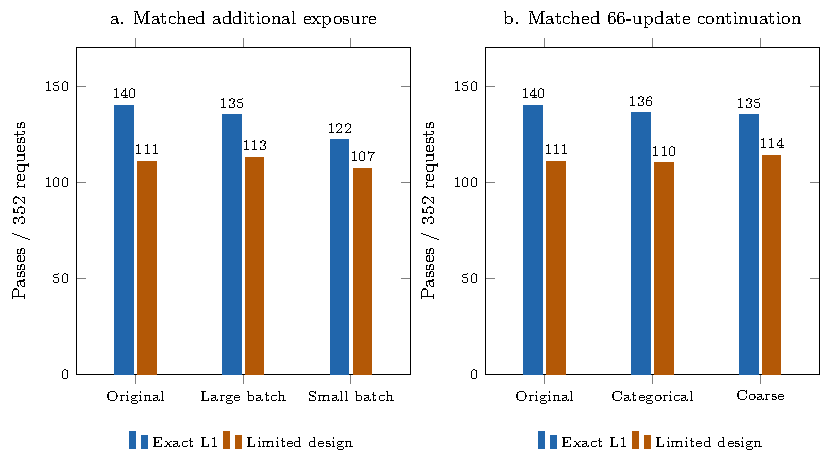
\includegraphics[width=\textwidth]{figures/current_results/training_diagnostics.pdf}
\caption{\textbf{Fixed-endpoint continuation diagnostics on 352 development requests.}
The matched-presentation large/small-update pilot has D1 exact counts 135/122 and design counts
113/107, versus original 140/111. The separate categorical/coarse66 pilot gives 136/135 exact
and 110/114 design, versus the same original 140/111. These are paired continuations of one fit,
not independent training seeds; no sampling uncertainty bars or held-out claim is attached.}
\label{fig:22-training}\end{figure}

\subsection{Exact-L1 decomposition and failure accounting}
We report exact assembly outcomes for each family, registered program, training seed and inference
arm. Each request contributes to the denominator whether generation, decomposition or verification
succeeds. Alongside exact yield, we count valid and connected graphs, distinct exact products,
unique exact precursor roots and checked decomposition traces.
Candidate-search coverage is the fraction of requests for which a decomposition candidate is found;
verified decomposition coverage requires exact replay. Candidate precision counts passing checked
traces over all checked traces, with ambiguity and search censoring explicit. The replay rate among
already accepted exact traces is an implementation invariant, not an independent precision estimate.
We distinguish family-local product counts from counts deduplicated across all families. Equal-family
macro averages, pooled yields and worst-family outcomes use separate definitions. Independent training-seed variability remains unmeasured; the reported development outcomes derive from one full fit.

\begin{table}[H]
\caption{\textbf{Attempt-level readout outcomes on the fixed 352-request development cohort.} One original checkpoint; 16 TRAIN-derived requests per family. Raw is the flow endpoint, terminal is the $t=1$ argmax, and D1 is constrained readout. Every failed request remains in $N$.}
\label{tab:22-outcomes}
\centering\footnotesize\setlength{\tabcolsep}{3pt}\renewcommand{\arraystretch}{1.10}
\begin{tabular}{@{}>{\raggedright\arraybackslash}p{.29\textwidth}ccccccc@{}}
\toprule
Family & $N$ & \shortstack{Raw\\exact} & \shortstack{Terminal\\exact} & \shortstack{D1\\exact} & \shortstack{D1 valid +\\connected} & \shortstack{D1 distinct\\exact} & \shortstack{D1\\nonexact} \\
\midrule
A3 amine--aldehyde--alkyne & 16 & 2 & 2 & 11 & 13 & 11 & 5 \\
Acid--epoxide diester & 16 & 6 & 9 & 14 & 16 & 14 & 2 \\
AEMA & 16 & 4 & 4 & 4 & 16 & 4 & 12 \\
Aldehyde Ugi 3-CR & 16 & 11 & 12 & 14 & 16 & 14 & 2 \\
Aldehyde Ugi 4-CR & 16 & 7 & 9 & 14 & 16 & 14 & 2 \\
$\alpha$-Isocyanoester dihydroimidazole & 16 & 7 & 7 & 10 & 11 & 10 & 6 \\
Amine alkylation & 16 & 0 & 0 & 0 & 16 & 0 & 16 \\
Amine--epoxide & 16 & 0 & 0 & 0 & 15 & 0 & 16 \\
Aryl reductive amination & 16 & 0 & 0 & 0 & 16 & 0 & 16 \\
Aza-Michael acrylamide & 16 & 0 & 0 & 0 & 15 & 0 & 16 \\
Aza-Michael acrylate & 16 & 1 & 1 & 0 & 15 & 0 & 16 \\
Disulfide Michael & 16 & 0 & 0 & 0 & 13 & 0 & 16 \\
Epoxide O-acylation & 16 & 1 & 1 & 4 & 16 & 4 & 12 \\
iPhos & 16 & 9 & 9 & 13 & 15 & 13 & 3 \\
Ketone--isocyanide amide & 16 & 6 & 7 & 14 & 14 & 14 & 2 \\
Ketone Ugi 4-CR & 16 & 1 & 0 & 5 & 10 & 5 & 11 \\
Maleate & 16 & 0 & 0 & 0 & 11 & 0 & 16 \\
O-esterification & 16 & 7 & 8 & 8 & 16 & 8 & 8 \\
Passerini & 16 & 9 & 10 & 15 & 16 & 15 & 1 \\
Preassembled thiol-yne & 16 & 0 & 0 & 1 & 15 & 1 & 15 \\
Reductive amination & 16 & 0 & 0 & 1 & 14 & 1 & 15 \\
Thiolactone & 16 & 9 & 12 & 12 & 14 & 12 & 4 \\
\midrule
All requests & 352 & 80 & 91 & 140 & 319 & 140 & 212 \\
\bottomrule
\end{tabular}
\par\smallskip\raggedright\scriptsize
These outputs precede the larger proposal/selection pipeline used for the separate 1,408-product cohort. A failed exact check is not experimental evidence of unmakeability. Ambiguity, checked-trace precision and independent-seed failure distributions are retained as unmeasured endpoints (\PendingCell); replay among accepted exact traces is a verifier invariant, not a precision estimate.
\end{table}
\begin{table}[H]
\caption{\textbf{Current single-fit result and missing independent replications.} The first column is the adaptively selected 1,408-request cohort from seed 2026092401, not a fresh held-out evaluation. Two further independent fits and their matched inference remain unrun. Sampling seeds and continuations do not supply training-seed replication.}
\label{tab:22-seeds}
\centering\footnotesize\setlength{\tabcolsep}{3pt}\renewcommand{\arraystretch}{1.10}
\begin{tabular}{@{}>{\raggedright\arraybackslash}p{.31\textwidth}cccc@{}}
\toprule
Family & \shortstack{Existing fit\\exact / $N$} & \shortstack{Independent\\fit B} & \shortstack{Independent\\fit C} & \shortstack{Mean $\pm$\\sample SD} \\
\midrule
A3 amine--aldehyde--alkyne & 61/64 & \PendingCell & \PendingCell & \PendingCell \\
Acid--epoxide diester & 63/64 & \PendingCell & \PendingCell & \PendingCell \\
AEMA & 63/64 & \PendingCell & \PendingCell & \PendingCell \\
Aldehyde Ugi 3-CR & 63/64 & \PendingCell & \PendingCell & \PendingCell \\
Aldehyde Ugi 4-CR & 64/64 & \PendingCell & \PendingCell & \PendingCell \\
$\alpha$-Isocyanoester dihydroimidazole & 64/64 & \PendingCell & \PendingCell & \PendingCell \\
Amine alkylation & 62/64 & \PendingCell & \PendingCell & \PendingCell \\
Amine--epoxide & 64/64 & \PendingCell & \PendingCell & \PendingCell \\
Aryl reductive amination & 58/64 & \PendingCell & \PendingCell & \PendingCell \\
Aza-Michael acrylamide & 64/64 & \PendingCell & \PendingCell & \PendingCell \\
Aza-Michael acrylate & 64/64 & \PendingCell & \PendingCell & \PendingCell \\
Disulfide Michael & 63/64 & \PendingCell & \PendingCell & \PendingCell \\
Epoxide O-acylation & 63/64 & \PendingCell & \PendingCell & \PendingCell \\
iPhos & 64/64 & \PendingCell & \PendingCell & \PendingCell \\
Ketone--isocyanide amide & 64/64 & \PendingCell & \PendingCell & \PendingCell \\
Ketone Ugi 4-CR & 62/64 & \PendingCell & \PendingCell & \PendingCell \\
Maleate & 64/64 & \PendingCell & \PendingCell & \PendingCell \\
O-esterification & 64/64 & \PendingCell & \PendingCell & \PendingCell \\
Passerini & 64/64 & \PendingCell & \PendingCell & \PendingCell \\
Preassembled thiol-yne & 64/64 & \PendingCell & \PendingCell & \PendingCell \\
Reductive amination & 61/64 & \PendingCell & \PendingCell & \PendingCell \\
Thiolactone & 64/64 & \PendingCell & \PendingCell & \PendingCell \\
\bottomrule
\end{tabular}
\par\smallskip\raggedright\scriptsize
The existing selected cohort has 1,387/1,408 exact products. No multi-fit mean, sample standard deviation or confidence interval is estimated from this single fit. The prospective matched held-out values remain \PendingCell.
\end{table}

\subsection{Matched controls, native baselines and the three-family comparison}
\begin{table}[H]
\caption{\textbf{Paired inference-only cyclic program-ID control.} The same checkpoint, requests and random draws receive the true or cyclically reassigned program ID. True structural context and source verification remain fixed. Counts use D1; design denotes the limited structural/design checks.}
\label{tab:22-controls}
\centering\footnotesize\setlength{\tabcolsep}{3pt}\renewcommand{\arraystretch}{1.10}
\begin{tabular}{@{}>{\raggedright\arraybackslash}p{.31\textwidth}ccccc@{}}
\toprule
Family & $N$ & \shortstack{True ID\\exact} & \shortstack{Cyclic ID\\exact} & \shortstack{True ID\\design} & \shortstack{Cyclic ID\\design} \\
\midrule
A3 amine--aldehyde--alkyne & 16 & 11 & 9 & 7 & 5 \\
Acid--epoxide diester & 16 & 14 & 12 & 12 & 9 \\
AEMA & 16 & 4 & 3 & 4 & 2 \\
Aldehyde Ugi 3-CR & 16 & 14 & 11 & 6 & 8 \\
Aldehyde Ugi 4-CR & 16 & 14 & 13 & 6 & 5 \\
$\alpha$-Isocyanoester dihydroimidazole & 16 & 10 & 5 & 10 & 5 \\
Amine alkylation & 16 & 0 & 0 & 0 & 0 \\
Amine--epoxide & 16 & 0 & 0 & 0 & 0 \\
Aryl reductive amination & 16 & 0 & 0 & 0 & 0 \\
Aza-Michael acrylamide & 16 & 0 & 3 & 0 & 3 \\
Aza-Michael acrylate & 16 & 0 & 0 & 0 & 0 \\
Disulfide Michael & 16 & 0 & 0 & 0 & 0 \\
Epoxide O-acylation & 16 & 4 & 1 & 4 & 1 \\
iPhos & 16 & 13 & 11 & 13 & 11 \\
Ketone--isocyanide amide & 16 & 14 & 10 & 14 & 10 \\
Ketone Ugi 4-CR & 16 & 5 & 0 & 4 & 0 \\
Maleate & 16 & 0 & 0 & 0 & 0 \\
O-esterification & 16 & 8 & 7 & 8 & 7 \\
Passerini & 16 & 15 & 10 & 14 & 10 \\
Preassembled thiol-yne & 16 & 1 & 1 & 0 & 1 \\
Reductive amination & 16 & 1 & 0 & 1 & 0 \\
Thiolactone & 16 & 12 & 9 & 8 & 5 \\
\midrule
All requests & 352 & 140 & 105 & 111 & 82 \\
\bottomrule
\end{tabular}
\par\smallskip\raggedright\scriptsize
On all 352 requests, raw exact counts are 80 versus 71 and terminal-argmax counts are 91 versus 85. The intervention tests the incremental program-ID signal with correct core/role/layout/depth information. A consistent training/test label bijection would instead be a recoding. Independently trained true shared-null, finite-catalogue selector, matched/generous FACT, qualified native external baselines and the matched three-family bridge remain \PendingCell. Shared-null implementation tests are not trained-null performance.
\end{table}
The completed control comparisons use paired request distributions from one original fit. Independent training-seed ranges and uncertainty remain unmeasured. Training exposure, checkpoint selection, decoder opportunity
and source/planner budgets define the matched comparison. We distinguish supported native chemistry
from unavailable baseline coverage. A wrong reaction label supplied alongside correct roles and
reaction cores tests the incremental information in that label; a retrained null model additionally
removes the corresponding training signal.

\subsection{Decoder and structural-repair attribution}
\begin{table}[H]
\caption{\textbf{Readout, saved-candidate selection and repair attribution.} The 352-request readouts and 192-request repair study have distinct populations. They do not estimate a model improvement or independent realism.}
\label{tab:22-decoder}
\centering\footnotesize\setlength{\tabcolsep}{3pt}\renewcommand{\arraystretch}{1.10}
\begin{tabular}{@{}>{\raggedright\arraybackslash}p{.38\textwidth}ccc>{\raggedright\arraybackslash}p{.29\textwidth}@{}}
\toprule
Arm & $N$ & Exact & Design & Attribution \\
\midrule
Original raw endpoint & 352 & 80 & 61 & Same saved trajectories \\
Original terminal argmax & 352 & 91 & 74 & Same saved trajectories \\
Original D1 & 352 & 140 & 111 & Same saved trajectories \\
Original verified fallback & 352 & 145 & 116 & No new model/proposal calls \\
Categorical66 verified fallback & 352 & 143 & 116 & No new model/proposal calls \\
Coarse66 verified fallback & 352 & 142 & 120 & No new model/proposal calls \\
\midrule
Three-family repair identity control & 192 & 187 & 140 & Separate construction diagnostic \\
Ring-scheduled proposals & 192 & 187 & 146 & Separate construction diagnostic \\
Anchor-preserving proposals & 192 & 187 & 146 & Separate construction diagnostic \\
Equal-cost / no TRAIN-motif-prior control & \PendingCell & \PendingCell & \PendingCell & \PendingCell \\
\bottomrule
\end{tabular}
\par\smallskip\raggedright\scriptsize
Verified fallback retains an exact D1 candidate, otherwise takes an already exact raw endpoint, otherwise an already exact terminal argmax, otherwise retains the D1 failure. It rescues 5/7/7 original/categorical/coarse requests, with no new candidates or exact/design losses. The categorical phosphate-tail Shannon count falls from 9.1180 to 9.0757; cross-checkpoint diversity floors still fail. The repair study includes all 64 A3, aldehyde-Ugi4 and ketone-Ugi4 requests: design counts change 51/50/39 to 55/51/40. Both repair arms change the same six requests and preserve the declared integer diversity/novelty floors; three resulting structures differ between the ring and anchor arms without an additional design-pass gain. Equal proposal caps do not mean equal measured cost; the full study uses 7.209 CPU seconds, 84 source checks and 84 design checks. The changed molecules have no transferred routing verdict, and the official 1,408-product cohort is unchanged. Individual decoder-rule and matched-cost effects remain \PendingCell.
\end{table}
The inference analysis separates readout, component completion, local chemical proposals, ring-system
proposals and population selection. We retain original, proposed and selected graphs, with atom,
bond and topology edits, repeated-arm identities, rejected proposals and search limits. Every design
predicate is evaluated on the final graph because a later construction can undo an earlier correction.
Cost includes duplicate and failed proposals, source checks and selection. TRAIN local motifs used
as proposal priors are identified separately from independent evaluation references.

% Generated by build_quality_current.py. Hash ledger: current_quality_evidence.json.
\subsection{Current structural quality and design-condition evidence}
The selected development cohort contains 1,408 requests, 64 per family, from one trained checkpoint. All selected identities match the current routing cohort. These counts describe an adaptively inspected TRAIN-derived population, not independent-seed estimates or held-out quality certification. Saved denotes the preceding selection, not unconstrained raw generation; selected denotes the context-preserving selection. Subsequent ring-receipt completion changes assessment availability, not molecular identity. Unmeasured endpoints retain placeholders.
\begingroup\scriptsize\setlength{\tabcolsep}{2.5pt}\renewcommand{\arraystretch}{1.1}
\begin{longtable}{@{}>{\raggedright\arraybackslash}p{.27\textwidth}>{\raggedright\arraybackslash}p{.105\textwidth}>{\raggedright\arraybackslash}p{.105\textwidth}>{\raggedright\arraybackslash}p{.105\textwidth}>{\raggedright\arraybackslash}p{.07\textwidth}>{\raggedright\arraybackslash}p{.075\textwidth}>{\raggedright\arraybackslash}p{.115\textwidth}@{}}
\caption{\textbf{Structural outcomes on the current selected development cohort.}}\label{tab:22-structure}\\
\toprule
Family & Valid/conn. & Exact L1 & Design & Alert & Context & Design, no context \\
\midrule\endfirsthead
\multicolumn{7}{l}{Table~\ref{tab:22-structure}, continued}\\
\toprule
Family & Valid/conn. & Exact L1 & Design & Alert & Context & Design, no context \\
\midrule\endhead
\bottomrule\endfoot
A3 & 64/64 & 61/64 & 51/64 & 0/64 & 7/64 & 47/64 \\
Acid--epoxide & 64/64 & 63/64 & 63/64 & 0/64 & 0/64 & 63/64 \\
AEMA & 64/64 & 63/64 & 63/64 & 0/64 & 0/64 & 63/64 \\
Aldehyde Ugi3 & 64/64 & 63/64 & 63/64 & 0/64 & 3/64 & 60/64 \\
Aldehyde Ugi4 & 64/64 & 64/64 & 50/64 & 0/64 & 1/64 & 49/64 \\
$\alpha$-Isocyanoester & 64/64 & 64/64 & 64/64 & 0/64 & 1/64 & 63/64 \\
Amine alkylation & 64/64 & 62/64 & 61/64 & 0/64 & 0/64 & 61/64 \\
Amine--epoxide & 64/64 & 64/64 & 58/64 & 0/64 & 6/64 & 52/64 \\
Aryl reductive amination & 64/64 & 58/64 & 58/64 & 0/64 & 3/64 & 56/64 \\
Aza-Michael acrylamide & 64/64 & 64/64 & 64/64 & 0/64 & 0/64 & 64/64 \\
Aza-Michael acrylate & 64/64 & 64/64 & 64/64 & 0/64 & 1/64 & 63/64 \\
Disulfide Michael & 64/64 & 63/64 & 62/64 & 0/64 & 2/64 & 60/64 \\
Epoxide/O-acylation & 64/64 & 63/64 & 60/64 & 0/64 & 0/64 & 60/64 \\
iPhos & 64/64 & 64/64 & 64/64 & 0/64 & 1/64 & 63/64 \\
Ketone--isocyanide & 64/64 & 64/64 & 64/64 & 0/64 & 0/64 & 64/64 \\
Ketone Ugi4 & 64/64 & 62/64 & 39/64 & 0/64 & 10/64 & 33/64 \\
Maleate & 64/64 & 64/64 & 60/64 & 0/64 & 2/64 & 59/64 \\
O-esterification & 64/64 & 64/64 & 64/64 & 0/64 & 0/64 & 64/64 \\
Passerini & 64/64 & 64/64 & 64/64 & 0/64 & 1/64 & 63/64 \\
Preassembled thiol-yne & 64/64 & 64/64 & 64/64 & 0/64 & 0/64 & 64/64 \\
Reductive amination & 64/64 & 61/64 & 61/64 & 0/64 & 1/64 & 60/64 \\
Thiolactone & 64/64 & 64/64 & 63/64 & 0/64 & 2/64 & 61/64 \\
\midrule
All requests & 1408/1408 & 1387/1408 & 1324/1408 & 0/1408 & 41/1408 & 1292/1408 \\
\end{longtable}\endgroup
Design requires exact L1 and all applicable qualified chemical, head and ring checks. Zero narrow-alert failures do not establish stability. Context flags overlap: hydrated/hemiacetal carbon 24, peroxide bond 8, carbon with at least three oxygens 6, other allene 5, small unsaturated ring 1 and heteroatom cumulene 1. The source-library screen passes 29/29 controls from two studies and two families; 20 families lack controls. Ten controls are component-disjoint; none supplies individual-product characterization in this control set. Independent blinded structural review remains \PendingValue{blinded structural review}.
\begingroup\scriptsize\setlength{\tabcolsep}{2.5pt}\renewcommand{\arraystretch}{1.1}
\begin{longtable}{@{}>{\raggedright\arraybackslash}p{.255\textwidth}>{\raggedright\arraybackslash}p{.09\textwidth}>{\raggedright\arraybackslash}p{.10\textwidth}>{\raggedright\arraybackslash}p{.10\textwidth}>{\raggedright\arraybackslash}p{.105\textwidth}>{\raggedright\arraybackslash}p{.13\textwidth}>{\raggedright\arraybackslash}p{.14\textwidth}@{}}
\caption{\textbf{Scoped conditions and TRAIN-feature diagnostics. Size excludes inapplicable cases.}}\label{tab:22-conditions}\\
\toprule
Family & Head P/F & Cycle P/N & Size P/A & Atom mean (\%) & Ring supported/A & Exact + observed/N \\
\midrule\endfirsthead
\multicolumn{7}{l}{Table~\ref{tab:22-conditions}, continued}\\
\toprule
Family & Head P/F & Cycle P/N & Size P/A & Atom mean (\%) & Ring supported/A & Exact + observed/N \\
\midrule\endhead
\bottomrule\endfoot
A3 & Outside scope & 62/64 & 41/53 & 96.222 & 12/53 & 14/64 \\
Acid--epoxide & Outside scope & 64/64 & 33/33 & 98.307 & 31/33 & 38/64 \\
AEMA & Outside scope & 64/64 & 22/22 & 99.979 & 22/22 & 63/64 \\
Aldehyde Ugi3 & Outside scope & 64/64 & 47/47 & 98.088 & 39/47 & 31/64 \\
Aldehyde Ugi4 & 59/5 & 63/64 & 45/59 & 98.030 & 28/59 & 20/64 \\
$\alpha$-Isocyanoester & Outside scope & 64/64 & 43/43 & 98.593 & 62/64 & 50/64 \\
Amine alkylation & Outside scope & 64/64 & 30/31 & 99.119 & 27/31 & 51/64 \\
Amine--epoxide & Outside scope & 64/64 & 18/24 & 98.432 & 15/24 & 47/64 \\
Aryl reductive amination & Outside scope & 64/64 & 63/64 & 90.982 & 18/64 & 6/64 \\
Aza-Michael acrylamide & Outside scope & 64/64 & 24/24 & 99.855 & 23/24 & 63/64 \\
Aza-Michael acrylate & Outside scope & 64/64 & 19/19 & 99.910 & 19/19 & 61/64 \\
Disulfide Michael & Outside scope & 64/64 & 20/21 & 97.513 & 14/21 & 36/64 \\
Epoxide/O-acylation & Outside scope & 64/64 & 27/30 & 99.722 & 25/30 & 51/64 \\
iPhos & Outside scope & 64/64 & 0/0 & 99.483 & 0/0 & 56/64 \\
Ketone--isocyanide & Outside scope & 64/64 & 28/28 & 99.920 & 28/28 & 63/64 \\
Ketone Ugi4 & Outside scope & 63/64 & 31/56 & 97.019 & 23/56 & 7/64 \\
Maleate & Outside scope & 64/64 & 22/26 & 98.646 & 18/26 & 48/64 \\
O-esterification & Outside scope & 64/64 & 36/36 & 98.967 & 30/36 & 55/64 \\
Passerini & Outside scope & 64/64 & 39/39 & 99.924 & 39/39 & 63/64 \\
Preassembled thiol-yne & Outside scope & 64/64 & 49/49 & 99.877 & 47/49 & 55/64 \\
Reductive amination & Outside scope & 64/64 & 46/47 & 98.903 & 37/47 & 45/64 \\
Thiolactone & Outside scope & 64/64 & 37/38 & 99.699 & 32/38 & 51/64 \\
\midrule
All requests & 59/5 & 1404/1408 & 720/789 & 98.509 & 589/810 & 974/1408 \\
\end{longtable}\endgroup
P/F denotes pass/fail; $N$ includes every request and $A$ only applicable assessed cases. Head retention is qualified only for aldehyde Ugi4: 59 pass, five fail and 1,344 outside scope. Role-cycle allocation passes 1,404/1,408; all 1,408 have no unexpected cross-origin edge. Qualified fundamental ring size passes 720/789, fails 69 and is inapplicable to 619; no case is unassessed. The unchanged combined ring endpoint is 1,339 pass and 69 fail. Tree bases comprise 700 saved raw trees, 631 declared ordered reconstructions, 15 certified construction transports and 62 no-tree cases with no applicable variable-cycle size; reconstructed trees do not become sampled provenance.
Atom-environment coverage averages the supported-atom fraction over all 1,408 products (98.509\%); the atom-weighted fraction is 77,273/78,532 (98.397\%). Of 810 ring-containing products, 589 have every connected ring-bond signature in family TRAIN support and 221 contain an unknown signature. The other 598 products are ring-free and are not applicable ring-support successes. Thus nonvacuous supported products are 589/1,408 requests; the original no-unknown-signature definition, explicitly including ring-free products, gives (589+598)/1,408. At the ring-system occurrence level 753/1,002 are supported. Unknown support is neither chemical rejection nor independent realism. Exact-plus-observed additionally requires exact decomposition and all product/component features observed in their appropriate TRAIN references; its 974 successes do not establish independent lipid realism.
\subsection{Distributional agreement with synthetic CAL references}
The same 1,821 exact-source-qualified synthetic CAL references are used across arms. They predominantly share TRAIN components; only one reference is component-disjoint. This is a development distribution diagnostic. The available broad empirical reference and control panels contain 1,024 unique structures each, share all 12 study groups and contain 32 and 36 exact TRAIN overlaps, respectively. Source ancestry remains insufficient to admit an independent empirical panel.
\begingroup\scriptsize\setlength{\tabcolsep}{2.5pt}\renewcommand{\arraystretch}{1.1}
\begin{longtable}{@{}>{\raggedright\arraybackslash}p{.15\textwidth}>{\raggedright\arraybackslash}p{.12\textwidth}>{\raggedright\arraybackslash}p{.10\textwidth}>{\raggedright\arraybackslash}p{.10\textwidth}>{\raggedright\arraybackslash}p{.10\textwidth}>{\raggedright\arraybackslash}p{.13\textwidth}>{\raggedright\arraybackslash}p{.09\textwidth}>{\raggedright\arraybackslash}p{.10\textwidth}@{}}
\caption{\textbf{Fingerprint agreement and internal diversity, by family and saved arm.}}\label{tab:22-realism}\\
\toprule
Arm & Unique $G/R$ & Prec. (\%) & Cov. (\%) & Recall (\%) & Distinct/$N$ (\%) & Nearest & Diversity \\
\midrule\endfirsthead
\multicolumn{8}{l}{Table~\ref{tab:22-realism}, continued}\\
\toprule
Arm & Unique $G/R$ & Prec. (\%) & Cov. (\%) & Recall (\%) & Distinct/$N$ (\%) & Nearest & Diversity \\
\midrule\endhead
\bottomrule\endfoot
\multicolumn{8}{l}{\textbf{A3}; $N=64$ per arm}\\
Saved & 64/27 & 64.062 & 70.370 & 92.593 & 64.062 & 0.419 & 0.728 \\
Selected & 64/27 & 56.250 & 70.370 & 92.593 & 56.250 & 0.401 & 0.729 \\
TRAIN control & 64/27 & 98.438 & 81.481 & 96.296 & 98.438 & 0.535 & 0.639 \\
\multicolumn{8}{l}{\textbf{Acid--epoxide}; $N=64$ per arm}\\
Saved & 64/95 & 43.750 & 41.053 & 73.684 & 43.750 & 0.692 & 0.496 \\
Selected & 64/95 & 42.188 & 43.158 & 84.211 & 42.188 & 0.683 & 0.510 \\
TRAIN control & 64/95 & 81.250 & 56.842 & 96.842 & 81.250 & 0.740 & 0.536 \\
\multicolumn{8}{l}{\textbf{AEMA}; $N=64$ per arm}\\
Saved & 64/21 & 85.938 & 95.238 & 80.952 & 85.938 & 0.826 & 0.336 \\
Selected & 64/21 & 85.938 & 95.238 & 80.952 & 85.938 & 0.823 & 0.339 \\
TRAIN control & 64/21 & 70.312 & 76.190 & 71.429 & 70.312 & 0.768 & 0.416 \\
\multicolumn{8}{l}{\textbf{Aldehyde Ugi3}; $N=64$ per arm}\\
Saved & 64/12 & 68.750 & 100.000 & 75.000 & 68.750 & 0.715 & 0.441 \\
Selected & 64/12 & 73.438 & 100.000 & 83.333 & 73.438 & 0.707 & 0.451 \\
TRAIN control & 64/12 & 96.875 & 100.000 & 75.000 & 96.875 & 0.834 & 0.344 \\
\multicolumn{8}{l}{\textbf{Aldehyde Ugi4}; $N=64$ per arm}\\
Saved & 64/61 & 82.812 & 80.328 & 77.049 & 82.812 & 0.599 & 0.624 \\
Selected & 64/61 & 84.375 & 78.689 & 73.770 & 84.375 & 0.588 & 0.636 \\
TRAIN control & 64/61 & 98.438 & 90.164 & 88.525 & 98.438 & 0.612 & 0.686 \\
\multicolumn{8}{l}{\textbf{$\alpha$-Isocyanoester}; $N=64$ per arm}\\
Saved & 64/103 & 29.688 & 8.738 & 48.544 & 29.688 & 0.732 & 0.457 \\
Selected & 64/103 & 32.812 & 8.738 & 47.573 & 32.812 & 0.737 & 0.452 \\
TRAIN control & 64/103 & 39.062 & 12.621 & 48.544 & 39.062 & 0.780 & 0.431 \\
\multicolumn{8}{l}{\textbf{Amine alkylation}; $N=64$ per arm}\\
Saved & 64/171 & 40.625 & 15.205 & 85.965 & 40.625 & 0.600 & 0.526 \\
Selected & 64/171 & 42.188 & 15.789 & 86.550 & 42.188 & 0.599 & 0.522 \\
TRAIN control & 64/171 & 84.375 & 40.351 & 93.567 & 84.375 & 0.711 & 0.541 \\
\multicolumn{8}{l}{\textbf{Amine--epoxide}; $N=64$ per arm}\\
Saved & 64/111 & 68.750 & 40.541 & 92.793 & 68.750 & 0.595 & 0.657 \\
Selected & 64/111 & 70.312 & 43.243 & 92.793 & 70.312 & 0.605 & 0.654 \\
TRAIN control & 64/111 & 76.562 & 43.243 & 90.991 & 76.562 & 0.650 & 0.640 \\
\multicolumn{8}{l}{\textbf{Aryl reductive amination}; $N=64$ per arm}\\
Saved & 63/79 & 6.349 & 24.051 & 98.734 & 6.250 & 0.547 & 0.597 \\
Selected & 63/79 & 3.175 & 15.190 & 100.000 & 3.125 & 0.539 & 0.599 \\
TRAIN control & 64/79 & 39.062 & 50.633 & 98.734 & 39.062 & 0.794 & 0.466 \\
\multicolumn{8}{l}{\textbf{Aza-Michael acrylamide}; $N=64$ per arm}\\
Saved & 64/33 & 75.000 & 60.606 & 90.909 & 75.000 & 0.686 & 0.530 \\
Selected & 64/33 & 75.000 & 60.606 & 90.909 & 75.000 & 0.677 & 0.526 \\
TRAIN control & 64/33 & 70.312 & 48.485 & 87.879 & 70.312 & 0.631 & 0.505 \\
\multicolumn{8}{l}{\textbf{Aza-Michael acrylate}; $N=64$ per arm}\\
Saved & 64/11 & 100.000 & 100.000 & 72.727 & 100.000 & 0.536 & 0.539 \\
Selected & 64/11 & 100.000 & 100.000 & 72.727 & 100.000 & 0.536 & 0.539 \\
TRAIN control & 64/11 & 100.000 & 100.000 & 81.818 & 100.000 & 0.561 & 0.494 \\
\multicolumn{8}{l}{\textbf{Disulfide Michael}; $N=64$ per arm}\\
Saved & 64/128 & 18.750 & 14.062 & 61.719 & 18.750 & 0.573 & 0.589 \\
Selected & 64/128 & 15.625 & 14.062 & 61.719 & 15.625 & 0.570 & 0.593 \\
TRAIN control & 64/128 & 50.000 & 24.219 & 78.906 & 50.000 & 0.727 & 0.452 \\
\multicolumn{8}{l}{\textbf{Epoxide/O-acylation}; $N=64$ per arm}\\
Saved & 64/70 & 71.875 & 60.000 & 70.000 & 71.875 & 0.722 & 0.492 \\
Selected & 64/70 & 68.750 & 60.000 & 70.000 & 68.750 & 0.715 & 0.498 \\
TRAIN control & 64/70 & 87.500 & 84.286 & 90.000 & 87.500 & 0.742 & 0.526 \\
\multicolumn{8}{l}{\textbf{iPhos}; $N=64$ per arm}\\
Saved & 64/62 & 78.125 & 32.258 & 93.548 & 78.125 & 0.672 & 0.535 \\
Selected & 64/62 & 78.125 & 32.258 & 93.548 & 78.125 & 0.673 & 0.536 \\
TRAIN control & 64/62 & 98.438 & 67.742 & 95.161 & 98.438 & 0.746 & 0.505 \\
\multicolumn{8}{l}{\textbf{Ketone--isocyanide}; $N=64$ per arm}\\
Saved & 64/29 & 87.500 & 72.414 & 96.552 & 87.500 & 0.718 & 0.516 \\
Selected & 64/29 & 87.500 & 72.414 & 96.552 & 87.500 & 0.724 & 0.515 \\
TRAIN control & 64/29 & 76.562 & 55.172 & 100.000 & 76.562 & 0.703 & 0.534 \\
\multicolumn{8}{l}{\textbf{Ketone Ugi4}; $N=64$ per arm}\\
Saved & 64/29 & 1.562 & 3.448 & 86.207 & 1.562 & 0.405 & 0.695 \\
Selected & 64/29 & 1.562 & 3.448 & 86.207 & 1.562 & 0.405 & 0.695 \\
TRAIN control & 64/29 & 87.500 & 100.000 & 96.552 & 87.500 & 0.648 & 0.530 \\
\multicolumn{8}{l}{\textbf{Maleate}; $N=64$ per arm}\\
Saved & 64/49 & 81.250 & 59.184 & 85.714 & 81.250 & 0.631 & 0.627 \\
Selected & 64/49 & 81.250 & 59.184 & 85.714 & 81.250 & 0.631 & 0.627 \\
TRAIN control & 64/49 & 89.062 & 65.306 & 83.673 & 89.062 & 0.638 & 0.626 \\
\multicolumn{8}{l}{\textbf{O-esterification}; $N=64$ per arm}\\
Saved & 64/43 & 51.562 & 79.070 & 69.767 & 51.562 & 0.575 & 0.661 \\
Selected & 64/43 & 51.562 & 79.070 & 69.767 & 51.562 & 0.577 & 0.663 \\
TRAIN control & 64/43 & 48.438 & 53.488 & 95.349 & 48.438 & 0.506 & 0.653 \\
\multicolumn{8}{l}{\textbf{Passerini}; $N=64$ per arm}\\
Saved & 64/68 & 87.500 & 55.882 & 89.706 & 87.500 & 0.759 & 0.487 \\
Selected & 64/68 & 87.500 & 55.882 & 89.706 & 87.500 & 0.757 & 0.488 \\
TRAIN control & 64/68 & 87.500 & 50.000 & 97.059 & 87.500 & 0.713 & 0.534 \\
\multicolumn{8}{l}{\textbf{Preassembled thiol-yne}; $N=64$ per arm}\\
Saved & 64/379 & 20.312 & 2.111 & 70.712 & 20.312 & 0.617 & 0.590 \\
Selected & 64/379 & 23.438 & 2.639 & 72.296 & 23.438 & 0.620 & 0.588 \\
TRAIN control & 64/379 & 34.375 & 3.958 & 91.557 & 34.375 & 0.604 & 0.625 \\
\multicolumn{8}{l}{\textbf{Reductive amination}; $N=64$ per arm}\\
Saved & 64/144 & 39.062 & 22.222 & 86.806 & 39.062 & 0.664 & 0.563 \\
Selected & 64/144 & 39.062 & 22.222 & 86.806 & 39.062 & 0.664 & 0.563 \\
TRAIN control & 64/144 & 76.562 & 54.861 & 99.306 & 76.562 & 0.796 & 0.539 \\
\multicolumn{8}{l}{\textbf{Thiolactone}; $N=64$ per arm}\\
Saved & 64/96 & 53.125 & 48.958 & 90.625 & 53.125 & 0.810 & 0.404 \\
Selected & 64/96 & 51.562 & 47.917 & 88.542 & 51.562 & 0.806 & 0.411 \\
TRAIN control & 64/96 & 60.938 & 39.583 & 88.542 & 60.938 & 0.817 & 0.413 \\
\end{longtable}\endgroup
\begingroup\scriptsize\setlength{\tabcolsep}{2.5pt}\renewcommand{\arraystretch}{1.1}
\def\LTcaptype{}\stepcounter{LT@tables}
\begin{longtable}{@{}>{\raggedright\arraybackslash}p{.245\textwidth}>{\raggedright\arraybackslash}p{.10\textwidth}>{\raggedright\arraybackslash}p{.10\textwidth}>{\raggedright\arraybackslash}p{.09\textwidth}>{\raggedright\arraybackslash}p{.09\textwidth}>{\raggedright\arraybackslash}p{.09\textwidth}>{\raggedright\arraybackslash}p{.09\textwidth}>{\raggedright\arraybackslash}p{.095\textwidth}@{}}
\caption*{\textbf{Table~\ref{tab:22-realism}, continued. Descriptor-space synthetic-CAL development comparison.}}\\
\toprule
Family & Selected P & Selected C & Saved P & Saved C & TRAIN P & TRAIN C & Reference n \\
\midrule\endfirsthead
\multicolumn{8}{l}{Table~\ref{tab:22-realism}, continued}\\
\toprule
Family & Selected P & Selected C & Saved P & Saved C & TRAIN P & TRAIN C & Reference n \\
\midrule\endhead
\bottomrule\endfoot
A3 & 76.562 & 66.667 & 81.250 & 66.667 & 79.688 & 74.074 & 27 \\
Acid--epoxide & 59.375 & 18.947 & 60.938 & 17.895 & 60.938 & 30.526 & 95 \\
AEMA & 78.125 & 100.000 & 78.125 & 100.000 & 76.562 & 85.714 & 21 \\
Aldehyde Ugi3 & 82.812 & 100.000 & 85.938 & 100.000 & 96.875 & 100.000 & 12 \\
Aldehyde Ugi4 & 89.062 & 78.689 & 87.500 & 78.689 & 96.875 & 81.967 & 61 \\
$\alpha$-Isocyanoester & 9.375 & 8.738 & 9.375 & 8.738 & 35.938 & 20.388 & 103 \\
Amine alkylation & 14.062 & 1.754 & 17.188 & 1.754 & 57.812 & 7.018 & 171 \\
Amine--epoxide & 78.125 & 27.928 & 76.562 & 27.928 & 81.250 & 40.541 & 111 \\
Aryl reductive amination & 45.312 & 6.329 & 45.312 & 6.329 & 60.938 & 6.329 & 79 \\
Aza-Michael acrylamide & 54.688 & 21.212 & 51.562 & 21.212 & 37.500 & 24.242 & 33 \\
Aza-Michael acrylate & 85.938 & 45.455 & 85.938 & 45.455 & 84.375 & 45.455 & 11 \\
Disulfide Michael & 25.000 & 10.938 & 23.438 & 9.375 & 54.688 & 19.531 & 128 \\
Epoxide/O-acylation & 87.500 & 38.571 & 89.062 & 31.429 & 75.000 & 60.000 & 70 \\
iPhos & 93.750 & 27.419 & 93.750 & 27.419 & 100.000 & 41.935 & 62 \\
Ketone--isocyanide & 35.938 & 86.207 & 39.062 & 86.207 & 26.562 & 48.276 & 29 \\
Ketone Ugi4 & 46.875 & 72.414 & 46.875 & 72.414 & 87.500 & 100.000 & 29 \\
Maleate & 68.750 & 51.020 & 68.750 & 51.020 & 78.125 & 48.980 & 49 \\
O-esterification & 46.875 & 25.581 & 43.750 & 25.581 & 51.562 & 25.581 & 43 \\
Passerini & 82.812 & 29.412 & 82.812 & 30.882 & 82.812 & 36.765 & 68 \\
Preassembled thiol-yne & 56.250 & 8.707 & 53.125 & 8.971 & 75.000 & 7.124 & 379 \\
Reductive amination & 7.812 & 0.694 & 7.812 & 0.694 & 51.562 & 22.222 & 144 \\
Thiolactone & 82.812 & 46.875 & 81.250 & 42.708 & 81.250 & 40.625 & 96 \\
\end{longtable}\endgroup
Fingerprint precision is reference-neighborhood membership, not the probability that a molecule is chemically realistic. Large generated neighborhoods can inflate recall. TRAIN controls are not layout-matched independent controls. Descriptor P and C in the additional panel are percentages of generated observations contained in synthetic-CAL balls and reference balls hit by any generated observation. Balls use Euclidean distance over all 24 descriptors after a same-family TRAIN-control median/IQR scaling (population SD, then one for constant features), with fifth-nonself-neighbor radii and $10^{-12}$ tolerance. This is a new descriptive development estimate; the first 64 TRAIN controls fit scaling and are not independent validation. Independent empirical descriptor precision/coverage remain \PendingValue{independent descriptor precision/coverage}; source-grouped C2ST AUC and uncertainty remain \PendingValue{independent C2ST}.
\begingroup\scriptsize\setlength{\tabcolsep}{2.5pt}\renewcommand{\arraystretch}{1.1}
\def\LTcaptype{}\stepcounter{LT@tables}
\begin{longtable}{@{}>{\raggedright\arraybackslash}p{.20\textwidth}>{\raggedright\arraybackslash}p{.11\textwidth}>{\raggedright\arraybackslash}p{.15\textwidth}>{\raggedright\arraybackslash}p{.15\textwidth}>{\raggedright\arraybackslash}p{.15\textwidth}>{\raggedright\arraybackslash}p{.16\textwidth}@{}}
\caption*{\textbf{Table~\ref{tab:22-realism}, continued. Same-request first-draw readout distributions, $N=64$ per family and arm.}}\\
\toprule
Readout & Valid/unique & FP P/C (\%) & Descriptor P/C (\%) & Distinct FP/$N$ & Descriptor obs./$N$ \\
\midrule\endfirsthead
\multicolumn{6}{l}{Table~\ref{tab:22-realism}, continued}\\
\toprule
Readout & Valid/unique & FP P/C (\%) & Descriptor P/C (\%) & Distinct FP/$N$ & Descriptor obs./$N$ \\
\midrule\endhead
\bottomrule\endfoot
\multicolumn{6}{l}{\textbf{A3}; reference observations 27}\\
Conditioned raw & 16/16 & 75.0/51.9 & 75.0/44.4 & 12/64 & 12/64 \\
Conditioned terminal & 17/17 & 94.1/55.6 & 70.6/44.4 & 16/64 & 12/64 \\
Cyclic raw & 26/26 & 73.1/44.4 & 84.6/48.1 & 19/64 & 22/64 \\
Cyclic terminal & 30/30 & 83.3/59.3 & 83.3/51.9 & 25/64 & 25/64 \\
\multicolumn{6}{l}{\textbf{Acid--epoxide}; reference observations 95}\\
Conditioned raw & 37/37 & 27.0/13.7 & 40.5/15.8 & 10/64 & 15/64 \\
Conditioned terminal & 46/46 & 37.0/16.8 & 54.3/16.8 & 17/64 & 25/64 \\
Cyclic raw & 46/46 & 30.4/17.9 & 30.4/13.7 & 14/64 & 14/64 \\
Cyclic terminal & 52/52 & 36.5/23.2 & 42.3/18.9 & 19/64 & 22/64 \\
\multicolumn{6}{l}{\textbf{AEMA}; reference observations 21}\\
Conditioned raw & 56/56 & 64.3/71.4 & 78.6/100.0 & 36/64 & 44/64 \\
Conditioned terminal & 62/62 & 61.3/71.4 & 77.4/100.0 & 38/64 & 48/64 \\
Cyclic raw & 53/53 & 60.4/95.2 & 75.5/100.0 & 32/64 & 40/64 \\
Cyclic terminal & 57/57 & 59.6/95.2 & 73.7/100.0 & 34/64 & 42/64 \\
\multicolumn{6}{l}{\textbf{Aldehyde Ugi3}; reference observations 12}\\
Conditioned raw & 55/55 & 56.4/100.0 & 83.6/100.0 & 31/64 & 46/64 \\
Conditioned terminal & 59/59 & 62.7/100.0 & 86.4/100.0 & 37/64 & 51/64 \\
Cyclic raw & 53/53 & 62.3/91.7 & 50.9/91.7 & 33/64 & 27/64 \\
Cyclic terminal & 59/59 & 67.8/100.0 & 52.5/83.3 & 40/64 & 31/64 \\
\multicolumn{6}{l}{\textbf{Aldehyde Ugi4}; reference observations 61}\\
Conditioned raw & 36/36 & 83.3/73.8 & 80.6/70.5 & 30/64 & 29/64 \\
Conditioned terminal & 39/39 & 92.3/75.4 & 94.9/75.4 & 36/64 & 37/64 \\
Cyclic raw & 35/35 & 74.3/59.0 & 82.9/70.5 & 26/64 & 29/64 \\
Cyclic terminal & 40/40 & 82.5/65.6 & 85.0/70.5 & 33/64 & 34/64 \\
\multicolumn{6}{l}{\textbf{$\alpha$-Isocyanoester}; reference observations 103}\\
Conditioned raw & 50/50 & 16.0/8.7 & 18.0/6.8 & 8/64 & 9/64 \\
Conditioned terminal & 56/55 & 21.8/9.7 & 19.6/8.7 & 12/64 & 11/64 \\
Cyclic raw & 50/50 & 10.0/8.7 & 4.0/2.9 & 5/64 & 2/64 \\
Cyclic terminal & 56/56 & 7.1/7.8 & 5.4/4.9 & 4/64 & 3/64 \\
\multicolumn{6}{l}{\textbf{Amine alkylation}; reference observations 171}\\
Conditioned raw & 38/38 & 2.6/1.8 & 0.0/0.0 & 1/64 & 0/64 \\
Conditioned terminal & 52/52 & 5.8/2.3 & 1.9/0.6 & 3/64 & 1/64 \\
Cyclic raw & 40/40 & 5.0/2.9 & 2.5/1.2 & 2/64 & 1/64 \\
Cyclic terminal & 50/50 & 12.0/3.5 & 4.0/1.8 & 6/64 & 2/64 \\
\multicolumn{6}{l}{\textbf{Amine--epoxide}; reference observations 111}\\
Conditioned raw & 34/34 & 44.1/10.8 & 97.1/27.9 & 15/64 & 33/64 \\
Conditioned terminal & 39/39 & 48.7/14.4 & 97.4/27.9 & 19/64 & 38/64 \\
Cyclic raw & 36/36 & 61.1/14.4 & 91.7/15.3 & 22/64 & 33/64 \\
Cyclic terminal & 41/41 & 63.4/15.3 & 90.2/21.6 & 26/64 & 37/64 \\
\multicolumn{6}{l}{\textbf{Aryl reductive amination}; reference observations 79}\\
Conditioned raw & 32/32 & 3.1/6.3 & 34.4/6.3 & 1/64 & 11/64 \\
Conditioned terminal & 50/50 & 10.0/20.3 & 38.0/6.3 & 5/64 & 19/64 \\
Cyclic raw & 28/28 & 0.0/0.0 & 10.7/6.3 & 0/64 & 3/64 \\
Cyclic terminal & 41/41 & 0.0/0.0 & 12.2/6.3 & 0/64 & 5/64 \\
\multicolumn{6}{l}{\textbf{Aza-Michael acrylamide}; reference observations 33}\\
Conditioned raw & 58/58 & 44.8/51.5 & 48.3/15.2 & 26/64 & 28/64 \\
Conditioned terminal & 58/58 & 50.0/54.5 & 53.4/18.2 & 29/64 & 31/64 \\
Cyclic raw & 59/59 & 47.5/45.5 & 42.4/36.4 & 28/64 & 25/64 \\
Cyclic terminal & 59/59 & 55.9/48.5 & 45.8/36.4 & 33/64 & 27/64 \\
\multicolumn{6}{l}{\textbf{Aza-Michael acrylate}; reference observations 11}\\
Conditioned raw & 52/52 & 94.2/100.0 & 92.3/45.5 & 49/64 & 48/64 \\
Conditioned terminal & 53/53 & 94.3/100.0 & 94.3/45.5 & 50/64 & 50/64 \\
Cyclic raw & 55/55 & 89.1/100.0 & 90.9/45.5 & 49/64 & 50/64 \\
Cyclic terminal & 58/58 & 94.8/100.0 & 93.1/45.5 & 55/64 & 54/64 \\
\multicolumn{6}{l}{\textbf{Disulfide Michael}; reference observations 128}\\
Conditioned raw & 16/16 & 0.0/0.0 & 25.0/1.6 & 0/64 & 4/64 \\
Conditioned terminal & 35/35 & 8.6/2.3 & 28.6/9.4 & 3/64 & 10/64 \\
Cyclic raw & 20/20 & 0.0/0.0 & 0.0/0.0 & 0/64 & 0/64 \\
Cyclic terminal & 40/40 & 0.0/0.0 & 7.5/5.5 & 0/64 & 3/64 \\
\multicolumn{6}{l}{\textbf{Epoxide/O-acylation}; reference observations 70}\\
Conditioned raw & 47/47 & 51.1/48.6 & 78.7/21.4 & 24/64 & 37/64 \\
Conditioned terminal & 48/47 & 59.6/50.0 & 79.2/21.4 & 28/64 & 38/64 \\
Cyclic raw & 44/44 & 27.3/28.6 & 72.7/25.7 & 12/64 & 32/64 \\
Cyclic terminal & 48/48 & 39.6/40.0 & 77.1/25.7 & 19/64 & 37/64 \\
\multicolumn{6}{l}{\textbf{iPhos}; reference observations 62}\\
Conditioned raw & 39/39 & 74.4/21.0 & 89.7/29.0 & 29/64 & 35/64 \\
Conditioned terminal & 42/42 & 81.0/21.0 & 88.1/27.4 & 34/64 & 37/64 \\
Cyclic raw & 45/45 & 60.0/16.1 & 82.2/29.0 & 27/64 & 37/64 \\
Cyclic terminal & 51/51 & 70.6/24.2 & 86.3/27.4 & 36/64 & 44/64 \\
\multicolumn{6}{l}{\textbf{Ketone--isocyanide}; reference observations 29}\\
Conditioned raw & 46/46 & 63.0/20.7 & 39.1/75.9 & 29/64 & 18/64 \\
Conditioned terminal & 49/49 & 67.3/20.7 & 36.7/75.9 & 33/64 & 18/64 \\
Cyclic raw & 57/57 & 45.6/27.6 & 24.6/48.3 & 26/64 & 14/64 \\
Cyclic terminal & 59/59 & 47.5/27.6 & 27.1/48.3 & 28/64 & 16/64 \\
\multicolumn{6}{l}{\textbf{Ketone Ugi4}; reference observations 29}\\
Conditioned raw & 8/8 & 0.0/0.0 & 50.0/24.1 & 0/64 & 4/64 \\
Conditioned terminal & 8/8 & 0.0/0.0 & 25.0/17.2 & 0/64 & 2/64 \\
Cyclic raw & 15/15 & 0.0/0.0 & 13.3/13.8 & 0/64 & 2/64 \\
Cyclic terminal & 26/26 & 0.0/0.0 & 46.2/41.4 & 0/64 & 12/64 \\
\multicolumn{6}{l}{\textbf{Maleate}; reference observations 49}\\
Conditioned raw & 27/27 & 51.9/36.7 & 66.7/24.5 & 14/64 & 18/64 \\
Conditioned terminal & 39/39 & 56.4/40.8 & 74.4/36.7 & 22/64 & 29/64 \\
Cyclic raw & 25/25 & 52.0/34.7 & 80.0/30.6 & 13/64 & 20/64 \\
Cyclic terminal & 35/35 & 54.3/38.8 & 74.3/36.7 & 19/64 & 26/64 \\
\multicolumn{6}{l}{\textbf{O-esterification}; reference observations 43}\\
Conditioned raw & 46/46 & 32.6/37.2 & 41.3/25.6 & 15/64 & 19/64 \\
Conditioned terminal & 49/49 & 34.7/37.2 & 40.8/25.6 & 17/64 & 20/64 \\
Cyclic raw & 43/43 & 46.5/39.5 & 48.8/25.6 & 20/64 & 21/64 \\
Cyclic terminal & 46/45 & 46.7/51.2 & 54.3/25.6 & 21/64 & 25/64 \\
\multicolumn{6}{l}{\textbf{Passerini}; reference observations 68}\\
Conditioned raw & 58/58 & 77.6/52.9 & 70.7/25.0 & 45/64 & 41/64 \\
Conditioned terminal & 59/59 & 86.4/54.4 & 72.9/26.5 & 51/64 & 43/64 \\
Cyclic raw & 60/60 & 73.3/48.5 & 60.0/25.0 & 44/64 & 36/64 \\
Cyclic terminal & 63/63 & 79.4/48.5 & 63.5/25.0 & 50/64 & 40/64 \\
\multicolumn{6}{l}{\textbf{Preassembled thiol-yne}; reference observations 379}\\
Conditioned raw & 37/37 & 5.4/0.8 & 48.6/4.0 & 2/64 & 18/64 \\
Conditioned terminal & 38/38 & 10.5/1.1 & 47.4/2.9 & 4/64 & 18/64 \\
Cyclic raw & 46/46 & 6.5/0.8 & 34.8/4.5 & 3/64 & 16/64 \\
Cyclic terminal & 50/50 & 10.0/0.8 & 28.0/3.7 & 5/64 & 14/64 \\
\multicolumn{6}{l}{\textbf{Reductive amination}; reference observations 144}\\
Conditioned raw & 29/29 & 10.3/4.2 & 24.1/3.5 & 3/64 & 7/64 \\
Conditioned terminal & 42/42 & 19.0/9.7 & 28.6/3.5 & 8/64 & 12/64 \\
Cyclic raw & 36/36 & 2.8/0.7 & 2.8/0.7 & 1/64 & 1/64 \\
Cyclic terminal & 44/44 & 2.3/0.7 & 2.3/0.7 & 1/64 & 1/64 \\
\multicolumn{6}{l}{\textbf{Thiolactone}; reference observations 96}\\
Conditioned raw & 49/49 & 38.8/38.5 & 79.6/37.5 & 19/64 & 39/64 \\
Conditioned terminal & 56/56 & 46.4/43.8 & 78.6/37.5 & 26/64 & 44/64 \\
Cyclic raw & 55/55 & 50.9/35.4 & 72.7/41.7 & 28/64 & 40/64 \\
Cyclic terminal & 62/62 & 58.1/42.7 & 74.2/37.5 & 36/64 & 46/64 \\
\end{longtable}\endgroup
The first-draw panel retains every one of the same 1,408 requests, including invalid outputs. Valid/unique reports connected observations and distinct connected constitutions; in this panel every valid serialized output is connected. FP precision conditions on unique connected products, descriptor precision on connected observations, and coverage on the corresponding family reference population. The last two columns keep all 64 requests in their denominators: distinct supported FP products and supported descriptor observations, respectively. Raw denotes the sampled flow endpoint; terminal denotes the final prediction argmax. Cyclic permutes program context at inference and is not a separately trained model. The selected panel above uses the original five draws and construction/selection rules; the first-draw contrast is therefore descriptive, not a matched-budget causal model comparison. Complete descriptor statistics and distances for every readout remain in the pinned evidence JSON. All selected-panel estimator values reproduce the preceding tables exactly.
\subsection{Definitions and interpretation of quality metrics}\label{app:22-metrics}
\begingroup\scriptsize\setlength{\tabcolsep}{2.5pt}\renewcommand{\arraystretch}{1.1}
\begin{longtable}{@{}>{\raggedright\arraybackslash}p{.29\textwidth}>{\raggedright\arraybackslash}p{.65\textwidth}@{}}
\caption{\textbf{Metric definitions and admitted scope.}}\label{tab:22-metric-definitions}\\
\toprule
Metric & Computation and limitation \\
\midrule\endfirsthead
\multicolumn{2}{l}{Table~\ref{tab:22-metric-definitions}, continued}\\
\toprule
Metric & Computation and limitation \\
\midrule\endhead
\bottomrule\endfoot
Valid molecules / all requests (\%) & RDKit parsing/sanitization; failure remains in all-request denominator. \\
Connected molecules / all requests (\%) & Exactly one connected molecular graph; distinct from validity. \\
Exact L1 + all qualified design checks / requests (\%) & Source-exact final graph and every applicable qualified axis assessed/pass. Unknowns and abstentions do not pass. \\
Molecules with a justified chemical alert / requests (\%) & Frozen narrow chemical-alert motifs; also report per-rule counts and unassessed requests. Not a complete stability screen. \\
Molecules requiring chemistry-context review / requests (\%) & Frozen context flags are descriptive, not automatic failures. \\
Required head retained / family-scope requests (\%) & Pass / prespecified family-scope requests; include charged or ambiguous-origin abstentions. Only neutral aldehyde-Ugi4 has a qualified predicate; other families remain unassessed. \\
Correct role-local cycle allocation / requests (\%) & Match declared variable closures per role, including zero; cross-origin edges must also match. All requests remain in denominator; report unassessed cases. \\
Requested ring-size agreement / comparable requests (\%) & Each observed fundamental-cycle length must belong to its role's allowed-size set, under a comparable tree basis. Not a size-multiset, SSSR or 3D-geometry match. Report inapplicable and unassessed counts. \\
TRAIN atom-environment coverage (\%) & Fraction of atoms with reference-observed local environments, averaged over assessed products. Report component-role summaries separately. \\
Ring-system TRAIN support / assessed products (\%) & Among valid connected products with a family TRAIN reference, fraction with no unknown connected ring-bond signature. Ring-free products pass vacuously; report them and missing/invalid cases separately. Component roles are separate. \\
Exact L1 + product/component features observed / requests (\%) & Exact, unambiguously decomposed product and every precursor must have all atom environments and connected ring-bond signatures observed in their family product or family/source-role TRAIN reference. Divide by all requests; absent references never pass. \\
Fingerprint precision (\%) & Fraction of unique generated molecules inside the union of reference k-nearest-neighbor balls in ECFP4/Tanimoto distance. \\
Fingerprint coverage (\%) & Fraction of reference-centered neighborhoods hit by at least one unique generated molecule. \\
Fingerprint recall (\%) & Fraction of references inside generated-centered neighborhoods. Distinct from coverage; small generated sets can inflate neighborhood radii. \\
Distinct reference-supported products / requests (\%) & Unique generated identities inside reference neighborhoods divided by all requests; exposes invalidity and duplication. \\
Nearest-reference Tanimoto similarity & Mean nearest-reference similarity over unique generated identities; descriptive, not a novelty or quality objective. \\
Internal ECFP4 diversity & Mean Tanimoto distance between distinct generated identities; compare alongside validity, realism and component diversity. \\
Descriptor distribution distance, per feature & One-dimensional Wasserstein distance / reference IQR; near-zero fallback: max(reference population SD,1). Connected-request observations retain duplicates. Smaller means closer to reference, not better chemistry. \\
Descriptor-space precision and coverage & Robust-scaled descriptor neighborhood metrics from the historical pipeline; new-model source-held-out reference/estimator contract and results remain pending. \\
Source-grouped two-sample classifier AUC & Distinguish generated and reference molecules with held-out source groups; classifier, sampling, leakage controls and final analysis are not yet qualified for the new model. \\
\end{longtable}\endgroup
Fingerprints are 2,048-bit Morgan fingerprints of radius two (ECFP4). Reference neighborhoods have radii equal to the fifth nonself reference-neighbor Tanimoto distance. Internal diversity is mean Tanimoto distance over distinct generated identity pairs. Descriptor $W_1/s_R$ divides one-dimensional Wasserstein distance by reference IQR; for IQR at most $10^{-12}$, $s_R=\max(\mathrm{SD}_{\mathrm{population}},1)$. Connected-request descriptor observations retain duplicates. No distribution distance is assigned an acceptability threshold.
\begingroup\scriptsize\setlength{\tabcolsep}{2.5pt}\renewcommand{\arraystretch}{1.1}
\begin{longtable}{@{}>{\raggedright\arraybackslash}p{.29\textwidth}>{\raggedright\arraybackslash}p{.085\textwidth}>{\raggedright\arraybackslash}p{.085\textwidth}>{\raggedright\arraybackslash}p{.085\textwidth}>{\raggedright\arraybackslash}p{.085\textwidth}>{\raggedright\arraybackslash}p{.09\textwidth}>{\raggedright\arraybackslash}p{.09\textwidth}>{\raggedright\arraybackslash}p{.09\textwidth}@{}}
\caption{\textbf{All 24 descriptor comparisons for every family.}}\label{tab:22-descriptors}\\
\toprule
Descriptor & $\mu_R$ & $\mu_S$ & $\mu_F$ & $\mu_T$ & $W_S/s_R$ & $W_F/s_R$ & $W_T/s_R$ \\
\midrule\endfirsthead
\multicolumn{8}{l}{Table~\ref{tab:22-descriptors}, continued}\\
\toprule
Descriptor & $\mu_R$ & $\mu_S$ & $\mu_F$ & $\mu_T$ & $W_S/s_R$ & $W_F/s_R$ & $W_T/s_R$ \\
\midrule\endhead
\bottomrule\endfoot
\multicolumn{8}{l}{\textbf{A3}; $n_R=27$, $n_S=n_F=n_T=64$}\\
Heavy atoms & 57.000 & 67.453 & 67.453 & 68.453 & 0.636 & 0.636 & 0.704 \\
Molecular weight & 789.498 & 942.287 & 942.195 & 951.521 & 0.680 & 0.679 & 0.729 \\
Calculated logP & 14.708 & 18.205 & 18.347 & 18.104 & 1.078 & 1.133 & 1.026 \\
Topological polar surface area & 43.113 & 55.977 & 54.450 & 58.942 & 0.627 & 0.562 & 0.685 \\
Hydrogen-bond donors & 0.667 & 0.703 & 0.641 & 0.656 & 0.483 & 0.452 & 0.124 \\
Hydrogen-bond acceptors & 4.259 & 5.156 & 5.094 & 5.172 & 0.624 & 0.591 & 0.614 \\
Rotatable bonds & 36.000 & 46.719 & 46.578 & 46.547 & 1.707 & 1.658 & 1.666 \\
Rings & 1.926 & 1.422 & 1.422 & 1.609 & 0.409 & 0.409 & 0.372 \\
Aromatic rings & 1.148 & 0.141 & 0.141 & 1.203 & 0.504 & 0.504 & 0.249 \\
Fraction sp$^3$ carbons & 0.788 & 0.870 & 0.870 & 0.813 & 0.529 & 0.528 & 0.222 \\
Net formal charge & 0.000 & 0.000 & 0.000 & 0.000 & 0.000 & 0.000 & 0.000 \\
Sum of absolute formal charges & 0.000 & 0.000 & 0.000 & 0.000 & 0.000 & 0.000 & 0.000 \\
Carbon fraction & 0.924 & 0.919 & 0.919 & 0.918 & 0.243 & 0.246 & 0.280 \\
Nitrogen atoms & 1.815 & 1.656 & 1.656 & 1.938 & 0.221 & 0.221 & 0.214 \\
Oxygen atoms & 2.444 & 3.625 & 3.562 & 3.609 & 0.787 & 0.745 & 0.777 \\
Sulfur atoms & 0.037 & 0.000 & 0.000 & 0.000 & 0.037 & 0.037 & 0.037 \\
Phosphorus atoms & 0.000 & 0.000 & 0.000 & 0.000 & 0.000 & 0.000 & 0.000 \\
Branching heavy atoms & 6.815 & 6.500 & 6.625 & 8.297 & 0.288 & 0.279 & 0.296 \\
Nonaromatic unsaturated bonds & 2.815 & 4.250 & 4.219 & 3.219 & 1.435 & 1.404 & 0.404 \\
Maximum polar-root distance & 19.296 & 22.734 & 22.797 & 18.891 & 0.875 & 0.891 & 0.178 \\
Heuristic head fraction & 0.229 & 0.215 & 0.226 & 0.216 & 0.293 & 0.255 & 0.276 \\
Heuristic interface fraction & 0.082 & 0.087 & 0.084 & 0.096 & 0.210 & 0.231 & 0.263 \\
Heuristic tail fraction & 0.689 & 0.698 & 0.691 & 0.688 & 0.238 & 0.221 & 0.206 \\
Heuristic tail branching atoms & 1.481 & 1.047 & 1.047 & 1.453 & 0.362 & 0.362 & 0.259 \\
\multicolumn{8}{l}{\textbf{Acid--epoxide}; $n_R=95$, $n_S=n_F=n_T=64$}\\
Heavy atoms & 42.695 & 44.922 & 44.922 & 45.094 & 0.290 & 0.290 & 0.299 \\
Molecular weight & 603.717 & 634.633 & 634.582 & 636.490 & 0.291 & 0.291 & 0.299 \\
Calculated logP & 10.204 & 10.087 & 10.029 & 10.091 & 0.229 & 0.231 & 0.182 \\
Topological polar surface area & 63.868 & 74.759 & 75.790 & 75.176 & 0.414 & 0.453 & 0.430 \\
Hydrogen-bond donors & 0.000 & 0.031 & 0.047 & 0.000 & 0.031 & 0.047 & 0.000 \\
Hydrogen-bond acceptors & 5.611 & 6.422 & 6.500 & 6.484 & 0.406 & 0.445 & 0.437 \\
Rotatable bonds & 30.253 & 32.312 & 32.047 & 30.984 & 0.299 & 0.261 & 0.177 \\
Rings & 0.463 & 0.516 & 0.516 & 0.578 & 0.052 & 0.052 & 0.115 \\
Aromatic rings & 0.000 & 0.000 & 0.000 & 0.000 & 0.000 & 0.000 & 0.000 \\
Fraction sp$^3$ carbons & 0.891 & 0.860 & 0.854 & 0.845 & 0.673 & 0.786 & 0.939 \\
Net formal charge & 0.000 & 0.000 & 0.000 & 0.000 & 0.000 & 0.000 & 0.000 \\
Sum of absolute formal charges & 0.000 & 0.000 & 0.000 & 0.000 & 0.000 & 0.000 & 0.000 \\
Carbon fraction & 0.866 & 0.856 & 0.854 & 0.856 & 0.196 & 0.213 & 0.149 \\
Nitrogen atoms & 1.000 & 1.047 & 1.062 & 1.000 & 0.047 & 0.062 & 0.000 \\
Oxygen atoms & 4.611 & 5.406 & 5.484 & 5.484 & 0.398 & 0.437 & 0.437 \\
Sulfur atoms & 0.000 & 0.000 & 0.000 & 0.000 & 0.000 & 0.000 & 0.000 \\
Phosphorus atoms & 0.000 & 0.000 & 0.000 & 0.000 & 0.000 & 0.000 & 0.000 \\
Branching heavy atoms & 5.168 & 4.938 & 5.000 & 5.453 & 0.292 & 0.266 & 0.438 \\
Nonaromatic unsaturated bonds & 3.137 & 4.047 & 4.156 & 4.312 & 0.910 & 1.019 & 1.176 \\
Maximum polar-root distance & 21.295 & 23.625 & 23.406 & 22.547 & 1.165 & 1.056 & 0.806 \\
Heuristic head fraction & 0.151 & 0.155 & 0.156 & 0.158 & 0.161 & 0.195 & 0.219 \\
Heuristic interface fraction & 0.186 & 0.203 & 0.206 & 0.200 & 0.237 & 0.257 & 0.179 \\
Heuristic tail fraction & 0.662 & 0.642 & 0.638 & 0.642 & 0.277 & 0.322 & 0.271 \\
Heuristic tail branching atoms & 0.737 & 0.188 & 0.188 & 0.797 & 0.549 & 0.549 & 0.250 \\
\multicolumn{8}{l}{\textbf{AEMA}; $n_R=21$, $n_S=n_F=n_T=64$}\\
Heavy atoms & 61.190 & 69.234 & 69.234 & 76.062 & 0.605 & 0.605 & 1.072 \\
Molecular weight & 904.249 & 1019.597 & 1019.597 & 1121.404 & 0.647 & 0.647 & 1.153 \\
Calculated logP & 10.288 & 13.409 & 13.403 & 13.699 & 0.445 & 0.444 & 0.487 \\
Topological polar surface area & 118.896 & 129.558 & 129.558 & 147.961 & 2.913 & 2.913 & 4.705 \\
Hydrogen-bond donors & 0.095 & 0.078 & 0.078 & 0.047 & 0.078 & 0.078 & 0.048 \\
Hydrogen-bond acceptors & 12.714 & 13.203 & 13.203 & 15.250 & 2.533 & 2.533 & 4.004 \\
Rotatable bonds & 41.952 & 51.484 & 51.453 & 54.781 & 0.590 & 0.588 & 0.813 \\
Rings & 0.524 & 0.344 & 0.344 & 0.422 & 0.180 & 0.180 & 0.102 \\
Aromatic rings & 0.048 & 0.047 & 0.047 & 0.016 & 0.001 & 0.001 & 0.032 \\
Fraction sp$^3$ carbons & 0.864 & 0.900 & 0.900 & 0.885 & 0.539 & 0.539 & 0.419 \\
Net formal charge & 0.000 & 0.000 & 0.000 & 0.000 & 0.000 & 0.000 & 0.000 \\
Sum of absolute formal charges & 0.000 & 0.000 & 0.000 & 0.000 & 0.000 & 0.000 & 0.000 \\
Carbon fraction & 0.786 & 0.808 & 0.808 & 0.800 & 0.323 & 0.323 & 0.228 \\
Nitrogen atoms & 2.286 & 1.875 & 1.875 & 2.234 & 0.411 & 0.411 & 0.261 \\
Oxygen atoms & 8.429 & 9.312 & 9.312 & 10.672 & 2.009 & 2.009 & 3.337 \\
Sulfur atoms & 2.048 & 2.062 & 2.062 & 2.359 & 0.359 & 0.359 & 0.624 \\
Phosphorus atoms & 0.000 & 0.000 & 0.000 & 0.000 & 0.000 & 0.000 & 0.000 \\
Branching heavy atoms & 9.619 & 8.891 & 8.938 & 11.031 & 1.129 & 1.170 & 2.068 \\
Nonaromatic unsaturated bonds & 5.286 & 5.016 & 5.016 & 6.172 & 0.551 & 0.551 & 0.596 \\
Maximum polar-root distance & 24.190 & 26.438 & 26.375 & 25.328 & 0.225 & 0.221 & 0.148 \\
Heuristic head fraction & 0.159 & 0.136 & 0.135 & 0.134 & 0.290 & 0.305 & 0.321 \\
Heuristic interface fraction & 0.256 & 0.234 & 0.234 & 0.245 & 0.304 & 0.301 & 0.203 \\
Heuristic tail fraction & 0.584 & 0.630 & 0.631 & 0.621 & 0.294 & 0.300 & 0.302 \\
Heuristic tail branching atoms & 3.190 & 2.391 & 2.438 & 3.359 & 0.348 & 0.329 & 0.408 \\
\multicolumn{8}{l}{\textbf{Aldehyde Ugi3}; $n_R=12$, $n_S=n_F=n_T=64$}\\
Heavy atoms & 55.083 & 45.891 & 45.891 & 47.328 & 6.128 & 6.128 & 5.170 \\
Molecular weight & 776.644 & 649.100 & 649.101 & 669.387 & 4.502 & 4.502 & 3.786 \\
Calculated logP & 13.015 & 10.124 & 10.114 & 10.517 & 1.930 & 1.937 & 1.668 \\
Topological polar surface area & 78.799 & 73.951 & 73.687 & 74.696 & 0.524 & 0.578 & 0.388 \\
Hydrogen-bond donors & 2.167 & 2.094 & 2.094 & 2.094 & 0.073 & 0.073 & 0.073 \\
Hydrogen-bond acceptors & 5.500 & 5.203 & 5.188 & 5.312 & 0.484 & 0.594 & 0.188 \\
Rotatable bonds & 42.333 & 34.859 & 35.016 & 36.172 & 1.759 & 1.722 & 1.450 \\
Rings & 1.167 & 0.734 & 0.734 & 0.734 & 0.432 & 0.432 & 0.432 \\
Aromatic rings & 0.083 & 0.031 & 0.031 & 0.047 & 0.052 & 0.052 & 0.036 \\
Fraction sp$^3$ carbons & 0.924 & 0.943 & 0.944 & 0.944 & 0.317 & 0.312 & 0.328 \\
Net formal charge & 0.000 & 0.000 & 0.000 & 0.000 & 0.000 & 0.000 & 0.000 \\
Sum of absolute formal charges & 0.000 & 0.000 & 0.000 & 0.000 & 0.000 & 0.000 & 0.000 \\
Carbon fraction & 0.880 & 0.864 & 0.864 & 0.865 & 0.937 & 0.921 & 0.871 \\
Nitrogen atoms & 3.333 & 3.141 & 3.141 & 3.266 & 0.193 & 0.193 & 0.068 \\
Oxygen atoms & 3.250 & 3.094 & 3.078 & 3.094 & 1.375 & 1.688 & 0.625 \\
Sulfur atoms & 0.000 & 0.000 & 0.000 & 0.000 & 0.000 & 0.000 & 0.000 \\
Phosphorus atoms & 0.000 & 0.000 & 0.000 & 0.000 & 0.000 & 0.000 & 0.000 \\
Branching heavy atoms & 4.750 & 4.172 & 4.172 & 4.172 & 0.289 & 0.289 & 0.289 \\
Nonaromatic unsaturated bonds & 2.667 & 2.062 & 2.047 & 2.047 & 0.302 & 0.310 & 0.310 \\
Maximum polar-root distance & 29.583 & 23.047 & 23.156 & 23.484 & 3.268 & 3.214 & 3.049 \\
Heuristic head fraction & 0.155 & 0.182 & 0.180 & 0.170 & 1.569 & 1.401 & 0.919 \\
Heuristic interface fraction & 0.130 & 0.149 & 0.149 & 0.145 & 1.471 & 1.439 & 1.015 \\
Heuristic tail fraction & 0.715 & 0.669 & 0.671 & 0.686 & 4.023 & 3.811 & 2.648 \\
Heuristic tail branching atoms & 0.000 & 0.047 & 0.031 & 0.000 & 0.047 & 0.031 & 0.000 \\
\multicolumn{8}{l}{\textbf{Aldehyde Ugi4}; $n_R=61$, $n_S=n_F=n_T=64$}\\
Heavy atoms & 47.705 & 46.484 & 46.484 & 45.484 & 0.163 & 0.163 & 0.181 \\
Molecular weight & 679.510 & 660.117 & 658.214 & 639.613 & 0.161 & 0.170 & 0.207 \\
Calculated logP & 9.265 & 9.572 & 9.486 & 8.667 & 0.099 & 0.088 & 0.143 \\
Topological polar surface area & 83.729 & 72.315 & 73.072 & 83.994 & 0.218 & 0.207 & 0.139 \\
Hydrogen-bond donors & 1.393 & 1.453 & 1.594 & 1.672 & 0.060 & 0.200 & 0.278 \\
Hydrogen-bond acceptors & 5.082 & 4.500 & 4.531 & 4.859 & 0.203 & 0.184 & 0.158 \\
Rotatable bonds & 28.066 & 28.828 & 28.828 & 26.000 & 0.125 & 0.134 & 0.258 \\
Rings & 1.951 & 1.984 & 2.016 & 2.281 & 0.093 & 0.123 & 0.439 \\
Aromatic rings & 0.459 & 0.125 & 0.125 & 0.750 & 0.334 & 0.334 & 0.291 \\
Fraction sp$^3$ carbons & 0.868 & 0.906 & 0.902 & 0.842 & 0.346 & 0.317 & 0.227 \\
Net formal charge & 0.000 & 0.000 & 0.000 & 0.000 & 0.000 & 0.000 & 0.000 \\
Sum of absolute formal charges & 0.000 & 0.000 & 0.000 & 0.000 & 0.000 & 0.000 & 0.000 \\
Carbon fraction & 0.841 & 0.855 & 0.854 & 0.836 & 0.218 & 0.207 & 0.155 \\
Nitrogen atoms & 3.492 & 3.531 & 3.594 & 3.969 & 0.274 & 0.199 & 0.477 \\
Oxygen atoms & 3.754 & 3.000 & 2.969 & 3.203 & 0.251 & 0.262 & 0.184 \\
Sulfur atoms & 0.115 & 0.031 & 0.047 & 0.078 & 0.084 & 0.068 & 0.037 \\
Phosphorus atoms & 0.000 & 0.000 & 0.000 & 0.000 & 0.000 & 0.000 & 0.000 \\
Branching heavy atoms & 8.787 & 7.438 & 7.438 & 8.734 & 0.337 & 0.337 & 0.120 \\
Nonaromatic unsaturated bonds & 3.180 & 2.797 & 2.844 & 2.844 & 0.192 & 0.168 & 0.168 \\
Maximum polar-root distance & 18.459 & 18.922 & 19.078 & 17.562 & 0.172 & 0.157 & 0.155 \\
Heuristic head fraction & 0.179 & 0.184 & 0.178 & 0.179 & 0.156 & 0.147 & 0.145 \\
Heuristic interface fraction & 0.208 & 0.185 & 0.186 & 0.207 & 0.483 & 0.471 & 0.101 \\
Heuristic tail fraction & 0.613 & 0.631 & 0.636 & 0.614 & 0.240 & 0.298 & 0.141 \\
Heuristic tail branching atoms & 1.639 & 1.141 & 1.141 & 1.547 & 0.207 & 0.207 & 0.072 \\
\multicolumn{8}{l}{\textbf{$\alpha$-Isocyanoester}; $n_R=103$, $n_S=n_F=n_T=64$}\\
Heavy atoms & 38.573 & 40.422 & 40.422 & 40.234 & 0.357 & 0.357 & 0.340 \\
Molecular weight & 542.886 & 569.510 & 569.840 & 565.588 & 0.357 & 0.359 & 0.332 \\
Calculated logP & 7.479 & 8.200 & 8.231 & 8.124 & 0.318 & 0.324 & 0.322 \\
Topological polar surface area & 60.667 & 60.012 & 59.381 & 59.300 & 0.086 & 0.093 & 0.042 \\
Hydrogen-bond donors & 0.000 & 0.250 & 0.203 & 0.000 & 0.250 & 0.203 & 0.000 \\
Hydrogen-bond acceptors & 6.204 & 6.078 & 6.062 & 6.109 & 0.100 & 0.112 & 0.046 \\
Rotatable bonds & 21.495 & 22.078 & 22.094 & 21.188 & 0.248 & 0.250 & 0.330 \\
Rings & 1.767 & 1.672 & 1.672 & 1.641 & 0.095 & 0.095 & 0.126 \\
Aromatic rings & 0.000 & 0.000 & 0.000 & 0.000 & 0.000 & 0.000 & 0.000 \\
Fraction sp$^3$ carbons & 0.895 & 0.907 & 0.910 & 0.882 & 0.234 & 0.256 & 0.191 \\
Net formal charge & 0.000 & 0.000 & 0.000 & 0.000 & 0.000 & 0.000 & 0.000 \\
Sum of absolute formal charges & 0.000 & 0.000 & 0.000 & 0.000 & 0.000 & 0.000 & 0.000 \\
Carbon fraction & 0.835 & 0.850 & 0.850 & 0.849 & 0.222 & 0.224 & 0.194 \\
Nitrogen atoms & 3.000 & 3.000 & 3.016 & 3.000 & 0.000 & 0.016 & 0.000 \\
Oxygen atoms & 3.204 & 3.078 & 3.047 & 3.109 & 0.100 & 0.116 & 0.046 \\
Sulfur atoms & 0.000 & 0.016 & 0.031 & 0.000 & 0.016 & 0.031 & 0.000 \\
Phosphorus atoms & 0.000 & 0.000 & 0.000 & 0.000 & 0.000 & 0.000 & 0.000 \\
Branching heavy atoms & 6.485 & 6.922 & 6.922 & 7.094 & 0.229 & 0.229 & 0.306 \\
Nonaromatic unsaturated bonds & 2.932 & 2.719 & 2.688 & 3.266 & 0.138 & 0.154 & 0.167 \\
Maximum polar-root distance & 10.417 & 13.312 & 13.344 & 10.328 & 0.724 & 0.732 & 0.123 \\
Heuristic head fraction & 0.336 & 0.308 & 0.308 & 0.318 & 0.351 & 0.351 & 0.251 \\
Heuristic interface fraction & 0.174 & 0.165 & 0.164 & 0.169 & 0.182 & 0.191 & 0.117 \\
Heuristic tail fraction & 0.490 & 0.527 & 0.528 & 0.513 & 0.302 & 0.308 & 0.288 \\
Heuristic tail branching atoms & 0.000 & 0.125 & 0.125 & 0.000 & 0.125 & 0.125 & 0.000 \\
\multicolumn{8}{l}{\textbf{Amine alkylation}; $n_R=171$, $n_S=n_F=n_T=64$}\\
Heavy atoms & 50.825 & 47.781 & 47.781 & 48.938 & 0.447 & 0.447 & 0.419 \\
Molecular weight & 715.903 & 675.129 & 675.019 & 689.989 & 0.443 & 0.444 & 0.424 \\
Calculated logP & 11.269 & 11.154 & 11.113 & 11.221 & 0.221 & 0.230 & 0.241 \\
Topological polar surface area & 64.281 & 59.754 & 59.809 & 60.671 & 0.490 & 0.485 & 0.391 \\
Hydrogen-bond donors & 0.070 & 0.031 & 0.031 & 0.031 & 0.039 & 0.039 & 0.039 \\
Hydrogen-bond acceptors & 6.491 & 6.000 & 6.016 & 6.125 & 0.491 & 0.476 & 0.366 \\
Rotatable bonds & 35.801 & 35.766 & 35.703 & 35.891 & 0.203 & 0.203 & 0.237 \\
Rings & 0.883 & 0.484 & 0.484 & 0.484 & 0.399 & 0.399 & 0.399 \\
Aromatic rings & 0.000 & 0.000 & 0.000 & 0.000 & 0.000 & 0.000 & 0.000 \\
Fraction sp$^3$ carbons & 0.858 & 0.904 & 0.902 & 0.869 & 1.761 & 1.725 & 0.720 \\
Net formal charge & 0.000 & 0.000 & 0.000 & 0.000 & 0.000 & 0.000 & 0.000 \\
Sum of absolute formal charges & 0.000 & 0.000 & 0.000 & 0.000 & 0.000 & 0.000 & 0.000 \\
Carbon fraction & 0.868 & 0.872 & 0.872 & 0.873 & 0.231 & 0.235 & 0.252 \\
Nitrogen atoms & 2.018 & 1.953 & 1.969 & 1.984 & 0.080 & 0.064 & 0.111 \\
Oxygen atoms & 4.474 & 4.047 & 4.047 & 4.141 & 0.427 & 0.427 & 0.333 \\
Sulfur atoms & 0.000 & 0.000 & 0.000 & 0.000 & 0.000 & 0.000 & 0.000 \\
Phosphorus atoms & 0.000 & 0.000 & 0.000 & 0.000 & 0.000 & 0.000 & 0.000 \\
Branching heavy atoms & 5.947 & 5.078 & 5.016 & 5.328 & 1.163 & 1.131 & 0.619 \\
Nonaromatic unsaturated bonds & 4.000 & 3.000 & 3.062 & 3.781 & 1.312 & 1.375 & 0.219 \\
Maximum polar-root distance & 15.357 & 16.938 & 16.984 & 16.547 & 0.527 & 0.543 & 0.397 \\
Heuristic head fraction & 0.200 & 0.211 & 0.212 & 0.208 & 0.604 & 0.581 & 0.491 \\
Heuristic interface fraction & 0.163 & 0.156 & 0.156 & 0.152 & 0.207 & 0.202 & 0.277 \\
Heuristic tail fraction & 0.637 & 0.633 & 0.632 & 0.641 & 0.213 & 0.209 & 0.222 \\
Heuristic tail branching atoms & 1.193 & 0.641 & 0.641 & 1.031 & 0.339 & 0.339 & 0.081 \\
\multicolumn{8}{l}{\textbf{Amine--epoxide}; $n_R=111$, $n_S=n_F=n_T=64$}\\
Heavy atoms & 54.856 & 56.078 & 56.078 & 54.281 & 0.565 & 0.565 & 0.431 \\
Molecular weight & 778.470 & 793.699 & 793.584 & 767.246 & 0.612 & 0.613 & 0.463 \\
Calculated logP & 9.041 & 12.229 & 12.121 & 10.437 & 0.477 & 0.461 & 0.225 \\
Topological polar surface area & 122.390 & 90.050 & 91.530 & 101.483 & 0.551 & 0.531 & 0.390 \\
Hydrogen-bond donors & 3.550 & 3.078 & 3.062 & 3.109 & 0.895 & 0.879 & 0.645 \\
Hydrogen-bond acceptors & 9.000 & 6.703 & 6.812 & 7.500 & 0.459 & 0.438 & 0.330 \\
Rotatable bonds & 38.829 & 44.078 & 43.891 & 39.188 & 0.846 & 0.837 & 0.489 \\
Rings & 0.378 & 0.375 & 0.375 & 0.266 & 0.003 & 0.003 & 0.113 \\
Aromatic rings & 0.009 & 0.062 & 0.062 & 0.016 & 0.053 & 0.053 & 0.007 \\
Fraction sp$^3$ carbons & 0.872 & 0.891 & 0.887 & 0.844 & 0.198 & 0.190 & 0.241 \\
Net formal charge & 0.000 & 0.000 & 0.000 & 0.000 & 0.000 & 0.000 & 0.000 \\
Sum of absolute formal charges & 0.000 & 0.000 & 0.000 & 0.000 & 0.000 & 0.000 & 0.000 \\
Carbon fraction & 0.832 & 0.871 & 0.870 & 0.859 & 0.426 & 0.407 & 0.304 \\
Nitrogen atoms & 2.072 & 2.062 & 2.078 & 1.953 & 0.269 & 0.285 & 0.244 \\
Oxygen atoms & 6.937 & 4.703 & 4.797 & 5.562 & 0.447 & 0.428 & 0.307 \\
Sulfur atoms & 0.000 & 0.000 & 0.000 & 0.000 & 0.000 & 0.000 & 0.000 \\
Phosphorus atoms & 0.000 & 0.000 & 0.000 & 0.000 & 0.000 & 0.000 & 0.000 \\
Branching heavy atoms & 8.441 & 6.328 & 6.406 & 7.484 & 0.325 & 0.313 & 0.186 \\
Nonaromatic unsaturated bonds & 3.937 & 2.594 & 2.750 & 4.203 & 0.336 & 0.297 & 0.226 \\
Maximum polar-root distance & 15.324 & 17.766 & 17.844 & 16.000 & 0.488 & 0.504 & 0.160 \\
Heuristic head fraction & 0.215 & 0.209 & 0.209 & 0.220 & 0.373 & 0.368 & 0.305 \\
Heuristic interface fraction & 0.197 & 0.133 & 0.135 & 0.152 & 0.417 & 0.404 & 0.292 \\
Heuristic tail fraction & 0.589 & 0.658 & 0.656 & 0.628 & 0.489 & 0.472 & 0.275 \\
Heuristic tail branching atoms & 0.541 & 0.656 & 0.656 & 1.172 & 0.171 & 0.171 & 0.548 \\
\multicolumn{8}{l}{\textbf{Aryl reductive amination}; $n_R=79$, $n_S=n_F=n_T=64$}\\
Heavy atoms & 61.468 & 63.094 & 63.094 & 63.312 & 0.329 & 0.329 & 0.321 \\
Molecular weight & 853.082 & 880.870 & 880.931 & 880.683 & 0.340 & 0.341 & 0.331 \\
Calculated logP & 14.686 & 13.541 & 13.519 & 14.608 & 1.224 & 1.233 & 1.123 \\
Topological polar surface area & 78.340 & 99.908 & 100.318 & 86.130 & 0.730 & 0.744 & 0.264 \\
Hydrogen-bond donors & 1.000 & 1.172 & 1.172 & 1.000 & 0.172 & 0.172 & 0.000 \\
Hydrogen-bond acceptors & 7.063 & 9.062 & 9.094 & 7.812 & 0.666 & 0.677 & 0.250 \\
Rotatable bonds & 40.608 & 40.641 & 40.578 & 40.797 & 0.908 & 0.917 & 0.837 \\
Rings & 1.354 & 1.766 & 1.766 & 1.562 & 0.411 & 0.411 & 0.208 \\
Aromatic rings & 1.000 & 0.984 & 0.984 & 1.000 & 0.016 & 0.016 & 0.000 \\
Fraction sp$^3$ carbons & 0.677 & 0.714 & 0.714 & 0.694 & 4.579 & 4.554 & 3.747 \\
Net formal charge & 0.000 & 0.000 & 0.000 & 0.000 & 0.000 & 0.000 & 0.000 \\
Sum of absolute formal charges & 0.000 & 0.000 & 0.000 & 0.000 & 0.000 & 0.000 & 0.000 \\
Carbon fraction & 0.885 & 0.853 & 0.853 & 0.874 & 1.787 & 1.826 & 0.658 \\
Nitrogen atoms & 2.354 & 2.656 & 2.656 & 2.562 & 0.302 & 0.302 & 0.208 \\
Oxygen atoms & 4.709 & 6.406 & 6.438 & 5.250 & 0.849 & 0.864 & 0.271 \\
Sulfur atoms & 0.000 & 0.000 & 0.000 & 0.000 & 0.000 & 0.000 & 0.000 \\
Phosphorus atoms & 0.000 & 0.000 & 0.000 & 0.000 & 0.000 & 0.000 & 0.000 \\
Branching heavy atoms & 7.190 & 9.250 & 9.281 & 8.797 & 0.687 & 0.697 & 0.536 \\
Nonaromatic unsaturated bonds & 6.937 & 5.906 & 5.906 & 6.500 & 0.472 & 0.472 & 0.146 \\
Maximum polar-root distance & 26.848 & 26.266 & 26.203 & 23.812 & 1.037 & 1.047 & 1.055 \\
Heuristic head fraction & 0.115 & 0.139 & 0.139 & 0.126 & 1.730 & 1.730 & 1.099 \\
Heuristic interface fraction & 0.142 & 0.179 & 0.181 & 0.164 & 0.927 & 0.970 & 0.544 \\
Heuristic tail fraction & 0.743 & 0.682 & 0.680 & 0.710 & 1.064 & 1.094 & 0.560 \\
Heuristic tail branching atoms & 1.772 & 2.484 & 2.469 & 2.172 & 0.931 & 0.915 & 0.722 \\
\multicolumn{8}{l}{\textbf{Aza-Michael acrylamide}; $n_R=33$, $n_S=n_F=n_T=64$}\\
Heavy atoms & 56.485 & 50.984 & 50.984 & 51.516 & 0.281 & 0.281 & 0.256 \\
Molecular weight & 796.183 & 718.038 & 717.959 & 723.960 & 0.283 & 0.283 & 0.259 \\
Calculated logP & 12.303 & 10.952 & 10.947 & 10.880 & 0.273 & 0.271 & 0.267 \\
Topological polar surface area & 91.703 & 76.298 & 76.495 & 77.410 & 0.800 & 0.790 & 0.764 \\
Hydrogen-bond donors & 3.182 & 2.516 & 2.516 & 2.484 & 0.666 & 0.666 & 0.697 \\
Hydrogen-bond acceptors & 4.758 & 4.312 & 4.328 & 4.312 & 0.601 & 0.586 & 0.633 \\
Rotatable bonds & 44.030 & 38.453 & 38.469 & 37.672 & 0.299 & 0.300 & 0.293 \\
Rings & 0.091 & 0.375 & 0.375 & 0.391 & 0.284 & 0.284 & 0.300 \\
Aromatic rings & 0.000 & 0.031 & 0.031 & 0.141 & 0.031 & 0.031 & 0.141 \\
Fraction sp$^3$ carbons & 0.882 & 0.883 & 0.883 & 0.852 & 0.206 & 0.169 & 0.340 \\
Net formal charge & 0.000 & 0.000 & 0.000 & 0.000 & 0.000 & 0.000 & 0.000 \\
Sum of absolute formal charges & 0.000 & 0.000 & 0.000 & 0.000 & 0.000 & 0.000 & 0.000 \\
Carbon fraction & 0.865 & 0.872 & 0.872 & 0.871 & 0.222 & 0.216 & 0.236 \\
Nitrogen atoms & 3.879 & 3.828 & 3.844 & 4.000 & 0.274 & 0.266 & 0.235 \\
Oxygen atoms & 3.303 & 2.609 & 2.609 & 2.562 & 0.694 & 0.694 & 0.741 \\
Sulfur atoms & 0.000 & 0.000 & 0.000 & 0.000 & 0.000 & 0.000 & 0.000 \\
Phosphorus atoms & 0.000 & 0.000 & 0.000 & 0.000 & 0.000 & 0.000 & 0.000 \\
Branching heavy atoms & 4.818 & 4.984 & 4.875 & 5.719 & 0.746 & 0.605 & 0.994 \\
Nonaromatic unsaturated bonds & 4.121 & 3.562 & 3.609 & 4.125 & 0.140 & 0.128 & 0.316 \\
Maximum polar-root distance & 19.636 & 18.703 & 18.938 & 18.500 & 0.187 & 0.195 & 0.250 \\
Heuristic head fraction & 0.161 & 0.175 & 0.175 & 0.172 & 0.230 & 0.231 & 0.221 \\
Heuristic interface fraction & 0.172 & 0.158 & 0.156 & 0.161 & 0.250 & 0.265 & 0.225 \\
Heuristic tail fraction & 0.668 & 0.667 & 0.669 & 0.666 & 0.236 & 0.243 & 0.245 \\
Heuristic tail branching atoms & 0.000 & 0.203 & 0.188 & 0.688 & 0.203 & 0.188 & 0.688 \\
\multicolumn{8}{l}{\textbf{Aza-Michael acrylate}; $n_R=11$, $n_S=n_F=n_T=64$}\\
Heavy atoms & 45.909 & 50.938 & 50.938 & 51.828 & 11.040 & 11.040 & 12.406 \\
Molecular weight & 649.262 & 719.685 & 719.622 & 731.559 & 8.991 & 8.969 & 10.113 \\
Calculated logP & 8.442 & 11.660 & 11.653 & 11.660 & 1.551 & 1.548 & 1.572 \\
Topological polar surface area & 83.094 & 73.323 & 73.323 & 74.899 & 0.466 & 0.466 & 0.387 \\
Hydrogen-bond donors & 0.273 & 0.516 & 0.516 & 0.562 & 0.486 & 0.486 & 0.580 \\
Hydrogen-bond acceptors & 7.636 & 6.547 & 6.547 & 6.672 & 0.726 & 0.726 & 0.643 \\
Rotatable bonds & 31.000 & 38.188 & 38.172 & 38.109 & 2.888 & 2.881 & 2.844 \\
Rings & 0.273 & 0.297 & 0.297 & 0.297 & 0.048 & 0.048 & 0.048 \\
Aromatic rings & 0.000 & 0.031 & 0.031 & 0.031 & 0.031 & 0.031 & 0.031 \\
Fraction sp$^3$ carbons & 0.825 & 0.882 & 0.880 & 0.863 & 0.816 & 0.798 & 0.609 \\
Net formal charge & 0.000 & 0.000 & 0.000 & 0.000 & 0.000 & 0.000 & 0.000 \\
Sum of absolute formal charges & 0.000 & 0.000 & 0.000 & 0.000 & 0.000 & 0.000 & 0.000 \\
Carbon fraction & 0.834 & 0.869 & 0.869 & 0.869 & 1.683 & 1.683 & 1.701 \\
Nitrogen atoms & 1.727 & 1.703 & 1.703 & 1.719 & 0.173 & 0.173 & 0.142 \\
Oxygen atoms & 5.909 & 4.875 & 4.875 & 4.984 & 2.068 & 2.068 & 1.849 \\
Sulfur atoms & 0.000 & 0.000 & 0.000 & 0.000 & 0.000 & 0.000 & 0.000 \\
Phosphorus atoms & 0.000 & 0.000 & 0.000 & 0.000 & 0.000 & 0.000 & 0.000 \\
Branching heavy atoms & 6.636 & 5.219 & 5.234 & 5.797 & 0.504 & 0.499 & 0.378 \\
Nonaromatic unsaturated bonds & 4.727 & 3.672 & 3.703 & 4.094 & 0.575 & 0.559 & 0.493 \\
Maximum polar-root distance & 14.909 & 18.484 & 18.438 & 17.281 & 1.022 & 1.008 & 0.678 \\
Heuristic head fraction & 0.185 & 0.175 & 0.173 & 0.169 & 0.316 & 0.336 & 0.350 \\
Heuristic interface fraction & 0.213 & 0.164 & 0.165 & 0.171 & 1.459 & 1.452 & 1.258 \\
Heuristic tail fraction & 0.601 & 0.661 & 0.662 & 0.660 & 4.837 & 4.916 & 4.580 \\
Heuristic tail branching atoms & 1.091 & 0.312 & 0.312 & 0.422 & 0.420 & 0.420 & 0.335 \\
\multicolumn{8}{l}{\textbf{Disulfide Michael}; $n_R=128$, $n_S=n_F=n_T=64$}\\
Heavy atoms & 74.820 & 88.672 & 88.672 & 83.828 & 1.798 & 1.798 & 1.421 \\
Molecular weight & 1169.589 & 1342.853 & 1341.749 & 1311.117 & 1.840 & 1.819 & 1.640 \\
Calculated logP & 14.594 & 20.048 & 20.283 & 16.331 & 1.086 & 1.133 & 0.390 \\
Topological polar surface area & 149.533 & 132.604 & 129.758 & 152.348 & 0.770 & 0.891 & 0.776 \\
Hydrogen-bond donors & 1.148 & 0.547 & 0.562 & 0.359 & 0.426 & 0.418 & 0.395 \\
Hydrogen-bond acceptors & 17.766 & 16.250 & 16.000 & 19.859 & 2.234 & 2.359 & 2.609 \\
Rotatable bonds & 56.539 & 70.719 & 70.719 & 62.516 & 1.719 & 1.719 & 0.999 \\
Rings & 0.203 & 0.375 & 0.375 & 0.359 & 0.203 & 0.203 & 0.250 \\
Aromatic rings & 0.125 & 0.062 & 0.031 & 0.109 & 0.062 & 0.094 & 0.078 \\
Fraction sp$^3$ carbons & 0.855 & 0.872 & 0.874 & 0.839 & 0.310 & 0.308 & 0.276 \\
Net formal charge & 0.000 & 0.000 & 0.000 & 0.000 & 0.000 & 0.000 & 0.000 \\
Sum of absolute formal charges & 0.000 & 0.000 & 0.000 & 0.000 & 0.000 & 0.000 & 0.000 \\
Carbon fraction & 0.760 & 0.806 & 0.808 & 0.760 & 0.842 & 0.890 & 0.127 \\
Nitrogen atoms & 1.164 & 2.016 & 2.000 & 2.172 & 0.852 & 0.836 & 1.008 \\
Oxygen atoms & 10.617 & 9.375 & 9.203 & 10.797 & 0.849 & 0.936 & 1.091 \\
Sulfur atoms & 6.047 & 5.031 & 4.969 & 6.984 & 2.109 & 2.016 & 0.938 \\
Phosphorus atoms & 0.000 & 0.000 & 0.000 & 0.000 & 0.000 & 0.000 & 0.000 \\
Branching heavy atoms & 8.609 & 8.297 & 8.172 & 10.203 & 0.273 & 0.320 & 0.797 \\
Nonaromatic unsaturated bonds & 6.047 & 6.719 & 6.562 & 7.453 & 1.255 & 1.147 & 1.214 \\
Maximum polar-root distance & 29.836 & 32.062 & 31.984 & 29.906 & 0.325 & 0.318 & 0.171 \\
Heuristic head fraction & 0.115 & 0.102 & 0.105 & 0.109 & 0.361 & 0.281 & 0.250 \\
Heuristic interface fraction & 0.285 & 0.232 & 0.227 & 0.284 & 0.732 & 0.800 & 0.126 \\
Heuristic tail fraction & 0.600 & 0.666 & 0.668 & 0.606 & 0.625 & 0.641 & 0.163 \\
Heuristic tail branching atoms & 2.297 & 1.891 & 1.859 & 2.797 & 0.750 & 0.750 & 0.500 \\
\multicolumn{8}{l}{\textbf{Epoxide/O-acylation}; $n_R=70$, $n_S=n_F=n_T=64$}\\
Heavy atoms & 61.443 & 75.484 & 75.484 & 72.266 & 2.006 & 2.006 & 1.546 \\
Molecular weight & 864.903 & 1063.155 & 1063.202 & 1015.782 & 1.884 & 1.885 & 1.434 \\
Calculated logP & 16.081 & 21.883 & 21.869 & 20.097 & 2.031 & 2.026 & 1.406 \\
Topological polar surface area & 62.028 & 59.160 & 59.353 & 60.118 & 0.515 & 0.483 & 0.357 \\
Hydrogen-bond donors & 0.000 & 0.016 & 0.016 & 0.000 & 0.016 & 0.016 & 0.000 \\
Hydrogen-bond acceptors & 6.143 & 5.984 & 6.000 & 6.109 & 0.228 & 0.213 & 0.103 \\
Rotatable bonds & 46.329 & 61.094 & 61.047 & 55.938 & 2.109 & 2.103 & 1.373 \\
Rings & 0.643 & 0.469 & 0.469 & 0.516 & 0.174 & 0.174 & 0.127 \\
Aromatic rings & 0.100 & 0.000 & 0.000 & 0.047 & 0.100 & 0.100 & 0.053 \\
Fraction sp$^3$ carbons & 0.883 & 0.934 & 0.935 & 0.895 & 0.708 & 0.718 & 0.306 \\
Net formal charge & 0.000 & 0.000 & 0.000 & 0.000 & 0.000 & 0.000 & 0.000 \\
Sum of absolute formal charges & 0.000 & 0.000 & 0.000 & 0.000 & 0.000 & 0.000 & 0.000 \\
Carbon fraction & 0.894 & 0.920 & 0.920 & 0.913 & 1.204 & 1.195 & 0.853 \\
Nitrogen atoms & 2.071 & 1.984 & 2.000 & 2.156 & 0.250 & 0.242 & 0.164 \\
Oxygen atoms & 4.171 & 4.000 & 4.000 & 4.000 & 0.171 & 0.171 & 0.171 \\
Sulfur atoms & 0.000 & 0.000 & 0.000 & 0.000 & 0.000 & 0.000 & 0.000 \\
Phosphorus atoms & 0.000 & 0.000 & 0.000 & 0.000 & 0.000 & 0.000 & 0.000 \\
Branching heavy atoms & 7.143 & 7.312 & 7.375 & 8.266 & 0.254 & 0.241 & 0.561 \\
Nonaromatic unsaturated bonds & 3.743 & 3.266 & 3.250 & 4.312 & 0.301 & 0.309 & 0.285 \\
Maximum polar-root distance & 15.486 & 19.594 & 19.656 & 17.375 & 0.587 & 0.596 & 0.270 \\
Heuristic head fraction & 0.173 & 0.137 & 0.137 & 0.147 & 0.393 & 0.395 & 0.297 \\
Heuristic interface fraction & 0.136 & 0.103 & 0.105 & 0.123 & 0.945 & 0.911 & 0.442 \\
Heuristic tail fraction & 0.690 & 0.759 & 0.758 & 0.731 & 0.754 & 0.743 & 0.444 \\
Heuristic tail branching atoms & 0.186 & 0.344 & 0.344 & 0.422 & 0.207 & 0.207 & 0.236 \\
\multicolumn{8}{l}{\textbf{iPhos}; $n_R=62$, $n_S=n_F=n_T=64$}\\
Heavy atoms & 44.742 & 49.766 & 49.766 & 51.234 & 3.522 & 3.522 & 3.330 \\
Molecular weight & 657.213 & 729.860 & 729.890 & 751.014 & 3.569 & 3.568 & 3.418 \\
Calculated logP & 8.758 & 12.750 & 12.730 & 12.318 & 2.865 & 2.856 & 2.433 \\
Topological polar surface area & 109.007 & 85.245 & 85.390 & 96.907 & 0.968 & 0.964 & 0.957 \\
Hydrogen-bond donors & 0.161 & 0.484 & 0.484 & 0.531 & 0.323 & 0.323 & 0.370 \\
Hydrogen-bond acceptors & 8.387 & 6.375 & 6.391 & 7.203 & 0.993 & 0.988 & 0.988 \\
Rotatable bonds & 33.548 & 41.688 & 41.672 & 40.859 & 3.406 & 3.411 & 2.772 \\
Rings & 0.000 & 0.000 & 0.000 & 0.000 & 0.000 & 0.000 & 0.000 \\
Aromatic rings & 0.000 & 0.000 & 0.000 & 0.000 & 0.000 & 0.000 & 0.000 \\
Fraction sp$^3$ carbons & 0.845 & 0.943 & 0.942 & 0.902 & 6.751 & 6.727 & 3.877 \\
Net formal charge & -0.935 & -0.938 & -0.938 & -1.016 & 0.211 & 0.211 & 0.258 \\
Sum of absolute formal charges & 1.258 & 1.469 & 1.469 & 1.516 & 0.211 & 0.211 & 0.258 \\
Carbon fraction & 0.780 & 0.836 & 0.835 & 0.828 & 3.526 & 3.500 & 3.078 \\
Nitrogen atoms & 1.097 & 1.219 & 1.219 & 1.266 & 0.122 & 0.122 & 0.169 \\
Oxygen atoms & 7.452 & 5.422 & 5.438 & 6.188 & 1.132 & 1.125 & 1.123 \\
Sulfur atoms & 0.000 & 0.000 & 0.000 & 0.000 & 0.000 & 0.000 & 0.000 \\
Phosphorus atoms & 1.097 & 1.203 & 1.203 & 1.266 & 0.106 & 0.106 & 0.169 \\
Branching heavy atoms & 4.016 & 2.656 & 2.672 & 3.859 & 1.025 & 1.013 & 0.798 \\
Nonaromatic unsaturated bonds & 4.532 & 2.578 & 2.578 & 3.656 & 1.487 & 1.487 & 1.107 \\
Maximum polar-root distance & 15.000 & 19.750 & 19.719 & 17.125 & 1.594 & 1.583 & 0.718 \\
Heuristic head fraction & 0.202 & 0.195 & 0.195 & 0.187 & 0.867 & 0.867 & 0.813 \\
Heuristic interface fraction & 0.232 & 0.147 & 0.147 & 0.160 & 4.896 & 4.872 & 4.098 \\
Heuristic tail fraction & 0.566 & 0.659 & 0.658 & 0.653 & 1.298 & 1.292 & 1.220 \\
Heuristic tail branching atoms & 0.113 & 0.047 & 0.047 & 0.281 & 0.066 & 0.066 & 0.168 \\
\multicolumn{8}{l}{\textbf{Ketone--isocyanide}; $n_R=29$, $n_S=n_F=n_T=64$}\\
Heavy atoms & 35.517 & 33.672 & 33.672 & 34.266 & 0.365 & 0.365 & 0.293 \\
Molecular weight & 498.826 & 474.605 & 474.652 & 482.682 & 0.358 & 0.358 & 0.289 \\
Calculated logP & 7.921 & 7.351 & 7.343 & 7.489 & 0.337 & 0.341 & 0.287 \\
Topological polar surface area & 44.370 & 44.366 & 44.558 & 44.370 & 0.004 & 0.188 & 0.000 \\
Hydrogen-bond donors & 2.000 & 2.000 & 2.016 & 2.000 & 0.000 & 0.016 & 0.000 \\
Hydrogen-bond acceptors & 3.000 & 3.000 & 3.016 & 3.000 & 0.000 & 0.016 & 0.000 \\
Rotatable bonds & 21.966 & 22.797 & 22.828 & 22.562 & 0.344 & 0.340 & 0.308 \\
Rings & 1.379 & 0.484 & 0.484 & 0.609 & 0.895 & 0.895 & 0.770 \\
Aromatic rings & 0.000 & 0.000 & 0.000 & 0.000 & 0.000 & 0.000 & 0.000 \\
Fraction sp$^3$ carbons & 0.915 & 0.911 & 0.912 & 0.911 & 0.230 & 0.222 & 0.210 \\
Net formal charge & 0.000 & 0.000 & 0.000 & 0.000 & 0.000 & 0.000 & 0.000 \\
Sum of absolute formal charges & 0.000 & 0.000 & 0.000 & 0.000 & 0.000 & 0.000 & 0.000 \\
Carbon fraction & 0.884 & 0.880 & 0.880 & 0.882 & 0.334 & 0.340 & 0.265 \\
Nitrogen atoms & 3.000 & 3.000 & 3.016 & 3.000 & 0.000 & 0.016 & 0.000 \\
Oxygen atoms & 1.000 & 1.000 & 1.000 & 1.000 & 0.000 & 0.000 & 0.000 \\
Sulfur atoms & 0.000 & 0.000 & 0.000 & 0.000 & 0.000 & 0.000 & 0.000 \\
Phosphorus atoms & 0.000 & 0.000 & 0.000 & 0.000 & 0.000 & 0.000 & 0.000 \\
Branching heavy atoms & 3.966 & 3.766 & 3.750 & 4.250 & 0.399 & 0.384 & 0.665 \\
Nonaromatic unsaturated bonds & 1.759 & 1.828 & 1.812 & 1.828 & 0.311 & 0.295 & 0.342 \\
Maximum polar-root distance & 14.379 & 14.047 & 14.062 & 13.688 & 0.357 & 0.337 & 0.357 \\
Heuristic head fraction & 0.229 & 0.201 & 0.201 & 0.202 & 0.551 & 0.535 & 0.525 \\
Heuristic interface fraction & 0.117 & 0.125 & 0.125 & 0.134 & 0.332 & 0.325 & 0.552 \\
Heuristic tail fraction & 0.654 & 0.674 & 0.673 & 0.664 & 0.331 & 0.311 & 0.253 \\
Heuristic tail branching atoms & 0.931 & 0.594 & 0.578 & 0.703 & 0.369 & 0.353 & 0.496 \\
\multicolumn{8}{l}{\textbf{Ketone Ugi4}; $n_R=29$, $n_S=n_F=n_T=64$}\\
Heavy atoms & 65.690 & 72.781 & 72.781 & 71.984 & 0.483 & 0.483 & 0.436 \\
Molecular weight & 917.762 & 1020.966 & 1020.966 & 1006.236 & 0.477 & 0.477 & 0.416 \\
Calculated logP & 11.939 & 15.606 & 15.606 & 13.763 & 0.610 & 0.610 & 0.351 \\
Topological polar surface area & 118.749 & 109.870 & 109.870 & 123.891 & 0.553 & 0.553 & 0.208 \\
Hydrogen-bond donors & 1.241 & 1.688 & 1.688 & 1.094 & 0.446 & 0.446 & 0.148 \\
Hydrogen-bond acceptors & 8.000 & 7.188 & 7.188 & 8.531 & 0.637 & 0.637 & 0.266 \\
Rotatable bonds & 37.724 & 48.641 & 48.641 & 42.234 & 0.646 & 0.646 & 0.298 \\
Rings & 1.552 & 2.234 & 2.234 & 2.016 & 0.357 & 0.357 & 0.233 \\
Aromatic rings & 0.000 & 0.000 & 0.000 & 0.000 & 0.000 & 0.000 & 0.000 \\
Fraction sp$^3$ carbons & 0.782 & 0.879 & 0.879 & 0.809 & 1.082 & 1.082 & 0.298 \\
Net formal charge & 0.000 & 0.000 & 0.000 & 0.000 & 0.000 & 0.000 & 0.000 \\
Sum of absolute formal charges & 0.000 & 0.000 & 0.000 & 0.000 & 0.000 & 0.000 & 0.000 \\
Carbon fraction & 0.845 & 0.871 & 0.871 & 0.851 & 0.702 & 0.702 & 0.215 \\
Nitrogen atoms & 3.138 & 3.266 & 3.266 & 3.203 & 0.128 & 0.128 & 0.065 \\
Oxygen atoms & 6.862 & 6.016 & 6.016 & 7.328 & 0.642 & 0.642 & 0.233 \\
Sulfur atoms & 0.000 & 0.000 & 0.000 & 0.000 & 0.000 & 0.000 & 0.000 \\
Phosphorus atoms & 0.000 & 0.000 & 0.000 & 0.000 & 0.000 & 0.000 & 0.000 \\
Branching heavy atoms & 9.931 & 10.219 & 10.219 & 10.969 & 0.291 & 0.291 & 0.274 \\
Nonaromatic unsaturated bonds & 8.138 & 5.656 & 5.656 & 8.094 & 1.241 & 1.241 & 0.140 \\
Maximum polar-root distance & 22.207 & 27.781 & 27.781 & 22.172 & 0.557 & 0.557 & 0.180 \\
Heuristic head fraction & 0.117 & 0.113 & 0.113 & 0.123 & 0.143 & 0.143 & 0.219 \\
Heuristic interface fraction & 0.225 & 0.179 & 0.179 & 0.212 & 0.694 & 0.694 & 0.243 \\
Heuristic tail fraction & 0.658 & 0.708 & 0.708 & 0.665 & 0.583 & 0.583 & 0.211 \\
Heuristic tail branching atoms & 1.862 & 3.656 & 3.656 & 2.625 & 0.600 & 0.600 & 0.254 \\
\multicolumn{8}{l}{\textbf{Maleate}; $n_R=49$, $n_S=n_F=n_T=64$}\\
Heavy atoms & 53.184 & 80.609 & 80.609 & 74.266 & 2.748 & 2.748 & 2.146 \\
Molecular weight & 754.986 & 1136.892 & 1136.892 & 1048.998 & 2.751 & 2.751 & 2.151 \\
Calculated logP & 10.219 & 18.488 & 18.488 & 14.621 & 1.760 & 1.760 & 0.939 \\
Topological polar surface area & 102.466 & 128.366 & 128.366 & 139.873 & 0.448 & 0.448 & 0.658 \\
Hydrogen-bond donors & 1.245 & 1.156 & 1.156 & 1.219 & 0.139 & 0.139 & 0.139 \\
Hydrogen-bond acceptors & 8.592 & 10.750 & 10.750 & 11.594 & 0.436 & 0.436 & 0.600 \\
Rotatable bonds & 38.061 & 61.734 & 61.734 & 52.859 & 6.072 & 6.072 & 4.384 \\
Rings & 0.367 & 0.406 & 0.406 & 0.531 & 0.039 & 0.039 & 0.164 \\
Aromatic rings & 0.000 & 0.000 & 0.000 & 0.000 & 0.000 & 0.000 & 0.000 \\
Fraction sp$^3$ carbons & 0.864 & 0.861 & 0.861 & 0.833 & 0.238 & 0.238 & 0.497 \\
Net formal charge & 0.000 & 0.000 & 0.000 & 0.000 & 0.000 & 0.000 & 0.000 \\
Sum of absolute formal charges & 0.000 & 0.000 & 0.000 & 0.000 & 0.000 & 0.000 & 0.000 \\
Carbon fraction & 0.837 & 0.861 & 0.861 & 0.841 & 0.283 & 0.283 & 0.119 \\
Nitrogen atoms & 2.102 & 2.516 & 2.516 & 2.703 & 0.289 & 0.289 & 0.301 \\
Oxygen atoms & 6.490 & 8.250 & 8.250 & 9.094 & 0.445 & 0.445 & 0.688 \\
Sulfur atoms & 0.122 & 0.016 & 0.016 & 0.047 & 0.107 & 0.107 & 0.076 \\
Phosphorus atoms & 0.000 & 0.000 & 0.000 & 0.000 & 0.000 & 0.000 & 0.000 \\
Branching heavy atoms & 7.224 & 8.328 & 8.328 & 10.156 & 0.344 & 0.344 & 0.733 \\
Nonaromatic unsaturated bonds & 4.653 & 6.969 & 6.969 & 7.500 & 0.579 & 0.579 & 0.712 \\
Maximum polar-root distance & 17.265 & 22.828 & 22.828 & 19.906 & 0.695 & 0.695 & 0.344 \\
Heuristic head fraction & 0.146 & 0.124 & 0.124 & 0.127 & 1.069 & 1.069 & 0.938 \\
Heuristic interface fraction & 0.219 & 0.171 & 0.171 & 0.213 & 0.522 & 0.522 & 0.161 \\
Heuristic tail fraction & 0.635 & 0.706 & 0.706 & 0.660 & 0.569 & 0.569 & 0.212 \\
Heuristic tail branching atoms & 0.571 & 0.938 & 0.938 & 1.344 & 0.320 & 0.320 & 0.676 \\
\multicolumn{8}{l}{\textbf{O-esterification}; $n_R=43$, $n_S=n_F=n_T=64$}\\
Heavy atoms & 33.581 & 36.688 & 36.688 & 35.812 & 0.571 & 0.571 & 0.539 \\
Molecular weight & 475.067 & 515.698 & 515.872 & 503.140 & 0.579 & 0.577 & 0.550 \\
Calculated logP & 6.520 & 8.807 & 8.817 & 8.224 & 1.189 & 1.203 & 0.951 \\
Topological polar surface area & 63.481 & 55.021 & 54.664 & 55.028 & 0.322 & 0.335 & 0.321 \\
Hydrogen-bond donors & 0.000 & 0.172 & 0.141 & 0.125 & 0.172 & 0.141 & 0.125 \\
Hydrogen-bond acceptors & 5.651 & 4.484 & 4.469 & 4.484 & 0.583 & 0.591 & 0.583 \\
Rotatable bonds & 22.279 & 25.250 & 25.219 & 23.641 & 0.563 & 0.552 & 0.519 \\
Rings & 0.093 & 0.562 & 0.562 & 0.594 & 0.469 & 0.469 & 0.501 \\
Aromatic rings & 0.000 & 0.328 & 0.328 & 0.391 & 0.328 & 0.328 & 0.391 \\
Fraction sp$^3$ carbons & 0.778 & 0.801 & 0.810 & 0.784 & 0.432 & 0.481 & 0.521 \\
Net formal charge & 0.000 & 0.000 & 0.000 & 0.000 & 0.000 & 0.000 & 0.000 \\
Sum of absolute formal charges & 0.000 & 0.000 & 0.000 & 0.000 & 0.000 & 0.000 & 0.000 \\
Carbon fraction & 0.826 & 0.861 & 0.861 & 0.856 & 2.625 & 2.690 & 2.348 \\
Nitrogen atoms & 1.093 & 1.438 & 1.422 & 1.500 & 0.344 & 0.329 & 0.407 \\
Oxygen atoms & 4.558 & 3.375 & 3.375 & 3.375 & 0.592 & 0.592 & 0.592 \\
Sulfur atoms & 0.000 & 0.000 & 0.000 & 0.000 & 0.000 & 0.000 & 0.000 \\
Phosphorus atoms & 0.000 & 0.000 & 0.000 & 0.000 & 0.000 & 0.000 & 0.000 \\
Branching heavy atoms & 4.326 & 4.344 & 4.312 & 4.828 & 0.532 & 0.485 & 0.251 \\
Nonaromatic unsaturated bonds & 3.907 & 3.250 & 3.156 & 3.266 & 2.198 & 2.323 & 1.541 \\
Maximum polar-root distance & 12.256 & 16.672 & 16.516 & 15.219 & 2.944 & 2.840 & 2.006 \\
Heuristic head fraction & 0.206 & 0.237 & 0.237 & 0.241 & 1.215 & 1.217 & 1.385 \\
Heuristic interface fraction & 0.235 & 0.160 & 0.160 & 0.177 & 1.051 & 1.047 & 0.811 \\
Heuristic tail fraction & 0.559 & 0.603 & 0.603 & 0.582 & 0.659 & 0.657 & 0.532 \\
Heuristic tail branching atoms & 0.000 & 0.125 & 0.125 & 0.219 & 0.125 & 0.125 & 0.219 \\
\multicolumn{8}{l}{\textbf{Passerini}; $n_R=68$, $n_S=n_F=n_T=64$}\\
Heavy atoms & 46.779 & 46.016 & 46.016 & 44.000 & 0.376 & 0.376 & 0.406 \\
Molecular weight & 656.738 & 646.808 & 646.840 & 618.064 & 0.369 & 0.369 & 0.398 \\
Calculated logP & 11.123 & 11.393 & 11.394 & 10.530 & 0.207 & 0.205 & 0.234 \\
Topological polar surface area & 64.383 & 60.911 & 60.911 & 60.745 & 1.267 & 1.267 & 1.154 \\
Hydrogen-bond donors & 1.000 & 1.000 & 1.000 & 1.000 & 0.000 & 0.000 & 0.000 \\
Hydrogen-bond acceptors & 4.603 & 4.203 & 4.203 & 4.172 & 0.462 & 0.462 & 0.462 \\
Rotatable bonds & 32.118 & 33.484 & 33.500 & 31.062 & 0.234 & 0.231 & 0.230 \\
Rings & 1.074 & 0.625 & 0.625 & 0.469 & 0.449 & 0.449 & 0.605 \\
Aromatic rings & 0.294 & 0.125 & 0.125 & 0.109 & 0.169 & 0.169 & 0.185 \\
Fraction sp$^3$ carbons & 0.858 & 0.863 & 0.864 & 0.836 & 0.144 & 0.143 & 0.218 \\
Net formal charge & 0.000 & 0.000 & 0.000 & 0.000 & 0.000 & 0.000 & 0.000 \\
Sum of absolute formal charges & 0.000 & 0.000 & 0.000 & 0.000 & 0.000 & 0.000 & 0.000 \\
Carbon fraction & 0.879 & 0.886 & 0.886 & 0.881 & 0.211 & 0.211 & 0.099 \\
Nitrogen atoms & 2.221 & 2.016 & 2.016 & 2.016 & 0.205 & 0.205 & 0.205 \\
Oxygen atoms & 3.382 & 3.188 & 3.188 & 3.156 & 0.226 & 0.226 & 0.226 \\
Sulfur atoms & 0.000 & 0.000 & 0.000 & 0.000 & 0.000 & 0.000 & 0.000 \\
Phosphorus atoms & 0.000 & 0.000 & 0.000 & 0.000 & 0.000 & 0.000 & 0.000 \\
Branching heavy atoms & 5.603 & 4.703 & 4.719 & 5.172 & 0.450 & 0.442 & 0.216 \\
Nonaromatic unsaturated bonds & 3.162 & 3.438 & 3.422 & 3.844 & 0.138 & 0.130 & 0.341 \\
Maximum polar-root distance & 22.029 & 23.750 & 23.719 & 21.125 & 0.423 & 0.416 & 0.234 \\
Heuristic head fraction & 0.183 & 0.166 & 0.166 & 0.159 & 0.365 & 0.365 & 0.478 \\
Heuristic interface fraction & 0.165 & 0.154 & 0.154 & 0.168 & 0.227 & 0.227 & 0.111 \\
Heuristic tail fraction & 0.652 & 0.680 & 0.680 & 0.673 & 0.413 & 0.413 & 0.317 \\
Heuristic tail branching atoms & 0.529 & 0.547 & 0.562 & 0.812 & 0.058 & 0.042 & 0.283 \\
\multicolumn{8}{l}{\textbf{Preassembled thiol-yne}; $n_R=379$, $n_S=n_F=n_T=64$}\\
Heavy atoms & 45.153 & 47.250 & 47.250 & 45.781 & 0.233 & 0.233 & 0.163 \\
Molecular weight & 670.309 & 698.470 & 698.549 & 677.574 & 0.236 & 0.237 & 0.165 \\
Calculated logP & 10.970 & 12.893 & 12.883 & 11.817 & 0.385 & 0.383 & 0.207 \\
Topological polar surface area & 37.218 & 30.360 & 29.861 & 31.857 & 0.617 & 0.604 & 0.410 \\
Hydrogen-bond donors & 0.491 & 0.734 & 0.672 & 0.578 & 0.244 & 0.181 & 0.087 \\
Hydrogen-bond acceptors & 5.042 & 4.109 & 4.125 & 4.422 & 0.933 & 0.917 & 0.620 \\
Rotatable bonds & 31.079 & 34.641 & 34.641 & 32.094 & 0.324 & 0.324 & 0.160 \\
Rings & 1.459 & 0.797 & 0.797 & 0.781 & 0.662 & 0.662 & 0.678 \\
Aromatic rings & 0.000 & 0.000 & 0.000 & 0.000 & 0.000 & 0.000 & 0.000 \\
Fraction sp$^3$ carbons & 0.931 & 0.910 & 0.911 & 0.886 & 0.249 & 0.239 & 0.528 \\
Net formal charge & 0.000 & 0.000 & 0.000 & 0.000 & 0.000 & 0.000 & 0.000 \\
Sum of absolute formal charges & 0.000 & 0.000 & 0.000 & 0.000 & 0.000 & 0.000 & 0.000 \\
Carbon fraction & 0.863 & 0.891 & 0.891 & 0.880 & 0.525 & 0.520 & 0.327 \\
Nitrogen atoms & 2.348 & 2.109 & 2.125 & 2.234 & 0.239 & 0.223 & 0.114 \\
Oxygen atoms & 1.694 & 1.000 & 1.000 & 1.188 & 0.694 & 0.694 & 0.506 \\
Sulfur atoms & 2.000 & 2.000 & 2.000 & 2.000 & 0.000 & 0.000 & 0.000 \\
Phosphorus atoms & 0.000 & 0.000 & 0.000 & 0.000 & 0.000 & 0.000 & 0.000 \\
Branching heavy atoms & 5.546 & 4.953 & 5.094 & 6.016 & 0.312 & 0.242 & 0.317 \\
Nonaromatic unsaturated bonds & 1.918 & 2.406 & 2.375 & 2.812 & 0.244 & 0.228 & 0.447 \\
Maximum polar-root distance & 22.325 & 23.719 & 23.672 & 21.562 & 0.235 & 0.230 & 0.214 \\
Heuristic head fraction & 0.222 & 0.179 & 0.178 & 0.188 & 0.588 & 0.591 & 0.456 \\
Heuristic interface fraction & 0.137 & 0.110 & 0.110 & 0.121 & 0.564 & 0.564 & 0.351 \\
Heuristic tail fraction & 0.641 & 0.712 & 0.712 & 0.691 & 0.669 & 0.671 & 0.468 \\
Heuristic tail branching atoms & 1.470 & 1.891 & 1.922 & 2.734 & 0.210 & 0.226 & 0.632 \\
\multicolumn{8}{l}{\textbf{Reductive amination}; $n_R=144$, $n_S=n_F=n_T=64$}\\
Heavy atoms & 55.681 & 60.703 & 60.703 & 60.016 & 0.390 & 0.390 & 0.345 \\
Molecular weight & 785.244 & 863.134 & 863.134 & 845.407 & 0.427 & 0.427 & 0.347 \\
Calculated logP & 11.628 & 10.618 & 10.618 & 12.630 & 0.395 & 0.395 & 0.610 \\
Topological polar surface area & 96.990 & 143.462 & 143.462 & 106.306 & 5.668 & 5.668 & 1.140 \\
Hydrogen-bond donors & 1.458 & 4.000 & 4.000 & 1.672 & 2.542 & 2.542 & 0.214 \\
Hydrogen-bond acceptors & 7.896 & 10.078 & 10.078 & 8.328 & 2.214 & 2.214 & 0.488 \\
Rotatable bonds & 39.264 & 45.125 & 45.125 & 42.891 & 0.652 & 0.652 & 0.446 \\
Rings & 0.847 & 0.766 & 0.766 & 0.844 & 0.314 & 0.314 & 0.361 \\
Aromatic rings & 0.410 & 0.062 & 0.062 & 0.297 & 0.347 & 0.347 & 0.113 \\
Fraction sp$^3$ carbons & 0.856 & 0.915 & 0.915 & 0.834 & 0.562 & 0.562 & 0.252 \\
Net formal charge & 0.000 & 0.000 & 0.000 & 0.000 & 0.000 & 0.000 & 0.000 \\
Sum of absolute formal charges & 0.000 & 0.000 & 0.000 & 0.000 & 0.000 & 0.000 & 0.000 \\
Carbon fraction & 0.856 & 0.832 & 0.832 & 0.856 & 0.679 & 0.679 & 0.308 \\
Nitrogen atoms & 2.278 & 1.984 & 1.984 & 2.203 & 0.293 & 0.293 & 0.075 \\
Oxygen atoms & 5.674 & 8.141 & 8.141 & 6.328 & 1.802 & 1.802 & 0.466 \\
Sulfur atoms & 0.000 & 0.000 & 0.000 & 0.000 & 0.000 & 0.000 & 0.000 \\
Phosphorus atoms & 0.000 & 0.000 & 0.000 & 0.000 & 0.000 & 0.000 & 0.000 \\
Branching heavy atoms & 7.632 & 7.734 & 7.734 & 7.094 & 0.293 & 0.293 & 0.538 \\
Nonaromatic unsaturated bonds & 3.556 & 3.250 & 3.250 & 4.969 & 0.224 & 0.224 & 0.707 \\
Maximum polar-root distance & 22.160 & 27.609 & 27.609 & 26.125 & 1.093 & 1.093 & 0.797 \\
Heuristic head fraction & 0.177 & 0.153 & 0.153 & 0.158 & 0.560 & 0.560 & 0.501 \\
Heuristic interface fraction & 0.160 & 0.191 & 0.191 & 0.172 & 0.581 & 0.581 & 0.230 \\
Heuristic tail fraction & 0.663 & 0.655 & 0.655 & 0.670 & 0.187 & 0.187 & 0.504 \\
Heuristic tail branching atoms & 1.306 & 1.719 & 1.719 & 0.750 & 0.207 & 0.207 & 0.278 \\
\multicolumn{8}{l}{\textbf{Thiolactone}; $n_R=96$, $n_S=n_F=n_T=64$}\\
Heavy atoms & 49.271 & 52.141 & 52.141 & 53.000 & 0.302 & 0.302 & 0.393 \\
Molecular weight & 713.537 & 752.610 & 752.814 & 764.816 & 0.297 & 0.298 & 0.388 \\
Calculated logP & 9.720 & 10.953 & 10.935 & 11.011 & 0.481 & 0.474 & 0.504 \\
Topological polar surface area & 89.150 & 88.147 & 88.345 & 90.397 & 0.562 & 0.503 & 0.385 \\
Hydrogen-bond donors & 1.906 & 1.953 & 1.953 & 2.000 & 0.047 & 0.047 & 0.094 \\
Hydrogen-bond acceptors & 6.271 & 6.109 & 6.141 & 6.250 & 0.161 & 0.130 & 0.021 \\
Rotatable bonds & 35.323 & 37.672 & 37.625 & 37.922 & 0.261 & 0.256 & 0.289 \\
Rings & 0.625 & 0.594 & 0.594 & 0.719 & 0.031 & 0.031 & 0.094 \\
Aromatic rings & 0.042 & 0.000 & 0.000 & 0.062 & 0.042 & 0.042 & 0.021 \\
Fraction sp$^3$ carbons & 0.886 & 0.874 & 0.877 & 0.878 & 0.311 & 0.245 & 0.251 \\
Net formal charge & 0.000 & 0.000 & 0.000 & 0.000 & 0.000 & 0.000 & 0.000 \\
Sum of absolute formal charges & 0.000 & 0.000 & 0.000 & 0.000 & 0.000 & 0.000 & 0.000 \\
Carbon fraction & 0.828 & 0.843 & 0.843 & 0.842 & 0.741 & 0.713 & 0.663 \\
Nitrogen atoms & 3.188 & 3.031 & 3.047 & 3.156 & 0.156 & 0.141 & 0.031 \\
Oxygen atoms & 4.125 & 4.078 & 4.094 & 4.156 & 0.047 & 0.031 & 0.031 \\
Sulfur atoms & 1.000 & 1.000 & 1.000 & 1.000 & 0.000 & 0.000 & 0.000 \\
Phosphorus atoms & 0.000 & 0.000 & 0.000 & 0.000 & 0.000 & 0.000 & 0.000 \\
Branching heavy atoms & 5.688 & 5.812 & 5.891 & 6.250 & 0.156 & 0.203 & 0.562 \\
Nonaromatic unsaturated bonds & 3.719 & 4.297 & 4.219 & 4.109 & 0.578 & 0.500 & 0.391 \\
Maximum polar-root distance & 25.833 & 27.031 & 26.859 & 26.391 & 0.299 & 0.257 & 0.181 \\
Heuristic head fraction & 0.151 & 0.147 & 0.147 & 0.147 & 0.195 & 0.212 & 0.224 \\
Heuristic interface fraction & 0.228 & 0.207 & 0.208 & 0.206 & 0.509 & 0.478 & 0.533 \\
Heuristic tail fraction & 0.621 & 0.646 & 0.644 & 0.647 & 0.341 & 0.325 & 0.337 \\
Heuristic tail branching atoms & 0.562 & 1.047 & 1.031 & 1.484 & 0.484 & 0.469 & 0.922 \\
\end{longtable}\endgroup
\begingroup\scriptsize\setlength{\tabcolsep}{2.5pt}\renewcommand{\arraystretch}{1.1}
\def\LTcaptype{}\stepcounter{LT@tables}
\begin{longtable}{@{}>{\raggedright\arraybackslash}p{.29\textwidth}>{\raggedright\arraybackslash}p{.315\textwidth}>{\raggedright\arraybackslash}p{.335\textwidth}@{}}
\caption*{\textbf{Table~\ref{tab:22-descriptors}, continued. Selected and synthetic-CAL descriptor dispersion.}}\\
\toprule
Descriptor & Reference: SD; median [Q1,Q3]; [P5,P95] & Selected: SD; median [Q1,Q3]; [P5,P95] \\
\midrule\endfirsthead
\multicolumn{3}{l}{Table~\ref{tab:22-descriptors}, continued}\\
\toprule
Descriptor & Reference: SD; median [Q1,Q3]; [P5,P95] & Selected: SD; median [Q1,Q3]; [P5,P95] \\
\midrule\endhead
\bottomrule\endfoot
\multicolumn{3}{l}{\textbf{A3}}\\
Heavy atoms & 9.48; 59 [46.5, 64]; [43.3, 66.4] & 29; 62 [52, 70]; [42.1, 101] \\
Molecular weight & 128; 812 [652, 890]; [603, 924] & 403; 865 [734, 978]; [592, 1.4e+03] \\
Calculated logP & 2.92; 15.3 [13.3, 16.7]; [10.1, 18.4] & 8.42; 17.1 [13.6, 20.3]; [9.81, 32.1] \\
Topological polar surface area & 18.2; 49.8 [29.7, 53]; [16.6, 69.3] & 34.3; 48 [29.5, 70.9]; [15.7, 119] \\
Hydrogen-bond donors & 0.555; 1 [0, 1]; [0, 1] & 0.966; 0 [0, 1]; [0, 2.85] \\
Hydrogen-bond acceptors & 1.51; 4 [3.5, 5]; [2.3, 6.7] & 2.64; 5 [3, 6]; [2, 9.85] \\
Rotatable bonds & 8.1; 35 [31.5, 38]; [24.9, 50.7] & 17.7; 45 [36.8, 54]; [24, 72.4] \\
Rings & 1.36; 3 [0.5, 3]; [0, 3] & 1.42; 1 [1, 2]; [0, 3.85] \\
Aromatic rings & 1.03; 2 [0, 2]; [0, 2] & 0.35; 0 [0, 0]; [0, 1] \\
Fraction sp$^3$ carbons & 0.0916; 0.75 [0.722, 0.878]; [0.661, 0.91] & 0.0562; 0.877 [0.841, 0.914]; [0.774, 0.931] \\
Net formal charge & 0; 0 [0, 0]; [0, 0] & 0; 0 [0, 0]; [0, 0] \\
Sum of absolute formal charges & 0; 0 [0, 0]; [0, 0] & 0; 0 [0, 0]; [0, 0] \\
Carbon fraction & 0.0277; 0.931 [0.907, 0.936]; [0.884, 0.957] & 0.0308; 0.922 [0.905, 0.94]; [0.852, 0.966] \\
Nitrogen atoms & 0.786; 2 [1, 2]; [1, 3] & 0.781; 2 [1, 2]; [1, 3] \\
Oxygen atoms & 1.48; 3 [1.5, 3]; [0, 4] & 2.4; 4 [2, 4]; [0.15, 7.85] \\
Sulfur atoms & 0.192; 0 [0, 0]; [0, 0] & 0; 0 [0, 0]; [0, 0] \\
Phosphorus atoms & 0; 0 [0, 0]; [0, 0] & 0; 0 [0, 0]; [0, 0] \\
Branching heavy atoms & 3.63; 8 [3, 10]; [2, 11] & 3.82; 6 [4, 8]; [3, 15.4] \\
Nonaromatic unsaturated bonds & 1.14; 3 [2, 3]; [1.3, 4.7] & 3.06; 3 [3, 5]; [2, 7.85] \\
Maximum polar-root distance & 2.58; 19 [17.5, 21.5]; [16, 23] & 4.47; 22.5 [19.8, 25]; [17, 31.8] \\
Heuristic head fraction & 0.0758; 0.231 [0.185, 0.264]; [0.123, 0.376] & 0.0732; 0.221 [0.18, 0.263]; [0.106, 0.352] \\
Heuristic interface fraction & 0.0491; 0.0952 [0.045, 0.103]; [0.00448, 0.156] & 0.0404; 0.0792 [0.0639, 0.106]; [0.0189, 0.162] \\
Heuristic tail fraction & 0.0929; 0.674 [0.626, 0.739]; [0.579, 0.864] & 0.0877; 0.693 [0.636, 0.754]; [0.544, 0.816] \\
Heuristic tail branching atoms & 1.55; 1 [0, 3]; [0, 3] & 2.45; 0 [0, 1]; [0, 7.1] \\
\multicolumn{3}{l}{\textbf{Acid--epoxide}}\\
Heavy atoms & 4.8; 45 [38, 47]; [36, 48] & 3.34; 45 [44, 47]; [39.1, 49] \\
Molecular weight & 65.7; 636 [540, 662]; [512, 676] & 47.3; 635 [619, 666]; [555, 695] \\
Calculated logP & 2.3; 9.82 [7.78, 12.3]; [7.16, 12.5] & 1.55; 10.1 [9.17, 10.9]; [7.27, 12.5] \\
Topological polar surface area & 12.8; 55.8 [55.8, 82.1]; [55.8, 82.1] & 18.5; 72.9 [55.8, 90]; [55.8, 108] \\
Hydrogen-bond donors & 0; 0 [0, 0]; [0, 0] & 0.213; 0 [0, 0]; [0, 0] \\
Hydrogen-bond acceptors & 0.971; 5 [5, 7]; [5, 7] & 1.3; 6 [5, 7]; [5, 9] \\
Rotatable bonds & 3.98; 31 [27, 34]; [25, 36] & 3.94; 32 [30, 35]; [25.1, 36.8] \\
Rings & 0.501; 0 [0, 1]; [0, 1] & 0.504; 1 [0, 1]; [0, 1] \\
Aromatic rings & 0; 0 [0, 0]; [0, 0] & 0; 0 [0, 0]; [0, 0] \\
Fraction sp$^3$ carbons & 0.0359; 0.905 [0.857, 0.907]; [0.833, 0.939] & 0.0637; 0.854 [0.814, 0.901]; [0.732, 0.944] \\
Net formal charge & 0; 0 [0, 0]; [0, 0] & 0; 0 [0, 0]; [0, 0] \\
Sum of absolute formal charges & 0; 0 [0, 0]; [0, 0] & 0; 0 [0, 0]; [0, 0] \\
Carbon fraction & 0.0341; 0.875 [0.823, 0.894]; [0.816, 0.896] & 0.0283; 0.856 [0.837, 0.873]; [0.8, 0.894] \\
Nitrogen atoms & 0; 1 [1, 1]; [1, 1] & 0.244; 1 [1, 1]; [1, 1.85] \\
Oxygen atoms & 0.971; 4 [4, 6]; [4, 6] & 1.3; 5 [4, 6]; [4, 8] \\
Sulfur atoms & 0; 0 [0, 0]; [0, 0] & 0; 0 [0, 0]; [0, 0] \\
Phosphorus atoms & 0; 0 [0, 0]; [0, 0] & 0; 0 [0, 0]; [0, 0] \\
Branching heavy atoms & 0.781; 5 [5, 6]; [4, 6.3] & 1.01; 5 [4, 6]; [4, 7] \\
Nonaromatic unsaturated bonds & 0.678; 3 [3, 4]; [2, 4] & 1.38; 4 [3, 5]; [2, 6.85] \\
Maximum polar-root distance & 1.71; 21 [20, 22]; [19, 24.3] & 2.54; 24 [22, 25]; [19, 26.8] \\
Heuristic head fraction & 0.0246; 0.154 [0.128, 0.17]; [0.105, 0.184] & 0.0272; 0.159 [0.146, 0.172]; [0.102, 0.187] \\
Heuristic interface fraction & 0.0507; 0.154 [0.149, 0.237]; [0.146, 0.263] & 0.0445; 0.193 [0.177, 0.236]; [0.149, 0.288] \\
Heuristic tail fraction & 0.0517; 0.681 [0.632, 0.708]; [0.563, 0.723] & 0.0471; 0.644 [0.608, 0.669]; [0.546, 0.715] \\
Heuristic tail branching atoms & 0.687; 1 [0, 1]; [0, 2] & 0.432; 0 [0, 0]; [0, 1] \\
\multicolumn{3}{l}{\textbf{AEMA}}\\
Heavy atoms & 10.4; 63 [53, 69]; [45, 71] & 23.2; 67.5 [55.8, 75]; [38, 106] \\
Molecular weight & 147; 929 [794, 1.02e+03]; [677, 1.05e+03] & 343; 993 [827, 1.1e+03]; [558, 1.57e+03] \\
Calculated logP & 3.89; 12.1 [5.85, 12.9]; [4.22, 14.7] & 5.02; 13.2 [9.94, 17.2]; [5.55, 21.5] \\
Topological polar surface area & 14.3; 112 [112, 121]; [112, 155] & 56.5; 112 [108, 161]; [62.3, 220] \\
Hydrogen-bond donors & 0.436; 0 [0, 0]; [0, 0] & 0.27; 0 [0, 0]; [0, 1] \\
Hydrogen-bond acceptors & 1.23; 12 [12, 13]; [12, 15] & 5.23; 12 [11, 15]; [8, 23] \\
Rotatable bonds & 10; 45 [34, 51]; [27, 55] & 18.7; 50 [38.8, 59]; [24.1, 77.8] \\
Rings & 0.512; 1 [0, 1]; [0, 1] & 0.479; 0 [0, 1]; [0, 1] \\
Aromatic rings & 0.218; 0 [0, 0]; [0, 0] & 0.213; 0 [0, 0]; [0, 0] \\
Fraction sp$^3$ carbons & 0.0816; 0.886 [0.86, 0.926]; [0.704, 0.931] & 0.0393; 0.912 [0.88, 0.929]; [0.816, 0.939] \\
Net formal charge & 0; 0 [0, 0]; [0, 0] & 0; 0 [0, 0]; [0, 0] \\
Sum of absolute formal charges & 0; 0 [0, 0]; [0, 0] & 0; 0 [0, 0]; [0, 0] \\
Carbon fraction & 0.0384; 0.806 [0.745, 0.814]; [0.723, 0.826] & 0.03; 0.806 [0.785, 0.826]; [0.765, 0.857] \\
Nitrogen atoms & 0.463; 2 [2, 3]; [2, 3] & 0.701; 2 [1, 2]; [1, 3] \\
Oxygen atoms & 0.978; 8 [8, 8]; [8, 10] & 4.24; 8 [8, 12]; [4, 16] \\
Sulfur atoms & 0.218; 2 [2, 2]; [2, 2] & 0.814; 2 [2, 2]; [1, 3.85] \\
Phosphorus atoms & 0; 0 [0, 0]; [0, 0] & 0; 0 [0, 0]; [0, 0] \\
Branching heavy atoms & 2.92; 8 [8, 9]; [8, 15] & 3.55; 8 [7, 10]; [5, 16.7] \\
Nonaromatic unsaturated bonds & 2.39; 4 [4, 4]; [4, 10] & 2.29; 4 [4, 6]; [2, 8.85] \\
Maximum polar-root distance & 6.13; 24 [18, 29]; [15, 32] & 3.68; 27 [24, 29]; [20, 31.8] \\
Heuristic head fraction & 0.0668; 0.127 [0.114, 0.194]; [0.0896, 0.277] & 0.0476; 0.119 [0.103, 0.175]; [0.076, 0.218] \\
Heuristic interface fraction & 0.0455; 0.238 [0.222, 0.298]; [0.212, 0.34] & 0.0394; 0.233 [0.206, 0.254]; [0.183, 0.306] \\
Heuristic tail fraction & 0.0998; 0.625 [0.509, 0.667]; [0.409, 0.686] & 0.0541; 0.64 [0.588, 0.675]; [0.53, 0.702] \\
Heuristic tail branching atoms & 2.52; 2 [2, 2]; [2, 8] & 1.51; 2 [2, 2]; [1, 5] \\
\multicolumn{3}{l}{\textbf{Aldehyde Ugi3}}\\
Heavy atoms & 2.47; 55 [54.8, 56.2]; [51.2, 57.9] & 4.44; 46 [43, 49]; [39.1, 52] \\
Molecular weight & 35.3; 776 [767, 795]; [722, 818] & 62.2; 652 [608, 695]; [555, 736] \\
Calculated logP & 1.51; 13.2 [12.4, 13.9]; [10.6, 14.9] & 1.76; 10.2 [8.95, 11.5]; [7.19, 13] \\
Topological polar surface area & 9.72; 76.9 [70.7, 81.2]; [70.7, 96.7] & 13.8; 70.7 [69.9, 79.9]; [53.6, 96.4] \\
Hydrogen-bond donors & 0.389; 2 [2, 2]; [2, 3] & 0.294; 2 [2, 2]; [2, 3] \\
Hydrogen-bond acceptors & 0.522; 5.5 [5, 6]; [5, 6] & 1.07; 5 [5, 6]; [4, 7] \\
Rotatable bonds & 2.53; 42.5 [40, 44.2]; [39.1, 45.5] & 4.18; 35 [33, 38]; [28, 40.8] \\
Rings & 0.937; 1 [1, 1]; [0, 3] & 0.445; 1 [0, 1]; [0, 1] \\
Aromatic rings & 0.289; 0 [0, 0]; [0, 0.45] & 0.175; 0 [0, 0]; [0, 0] \\
Fraction sp$^3$ carbons & 0.0544; 0.959 [0.874, 0.96]; [0.837, 0.961] & 0.0264; 0.95 [0.942, 0.955]; [0.889, 0.974] \\
Net formal charge & 0; 0 [0, 0]; [0, 0] & 0; 0 [0, 0]; [0, 0] \\
Sum of absolute formal charges & 0; 0 [0, 0]; [0, 0] & 0; 0 [0, 0]; [0, 0] \\
Carbon fraction & 0.0127; 0.876 [0.873, 0.891]; [0.863, 0.896] & 0.0244; 0.865 [0.85, 0.88]; [0.829, 0.898] \\
Nitrogen atoms & 0.492; 3 [3, 4]; [3, 4] & 0.467; 3 [3, 3]; [3, 4] \\
Oxygen atoms & 0.452; 3 [3, 3.25]; [3, 4] & 1.04; 3 [3, 4]; [1.15, 5] \\
Sulfur atoms & 0; 0 [0, 0]; [0, 0] & 0; 0 [0, 0]; [0, 0] \\
Phosphorus atoms & 0; 0 [0, 0]; [0, 0] & 0; 0 [0, 0]; [0, 0] \\
Branching heavy atoms & 0.965; 4 [4, 6]; [4, 6] & 0.808; 4 [4, 5]; [3, 6] \\
Nonaromatic unsaturated bonds & 0.985; 2 [2, 4]; [2, 4] & 0.653; 2 [2, 2]; [1, 3] \\
Maximum polar-root distance & 1.62; 30 [29, 31]; [26.6, 31] & 2.99; 23 [21.8, 25]; [19, 28] \\
Heuristic head fraction & 0.0102; 0.157 [0.145, 0.164]; [0.14, 0.165] & 0.0227; 0.18 [0.163, 0.197]; [0.144, 0.218] \\
Heuristic interface fraction & 0.011; 0.128 [0.124, 0.141]; [0.114, 0.144] & 0.0362; 0.147 [0.128, 0.17]; [0.0873, 0.199] \\
Heuristic tail fraction & 0.0118; 0.714 [0.709, 0.721]; [0.699, 0.732] & 0.0457; 0.674 [0.653, 0.699]; [0.586, 0.721] \\
Heuristic tail branching atoms & 0; 0 [0, 0]; [0, 0] & 0.175; 0 [0, 0]; [0, 0] \\
\multicolumn{3}{l}{\textbf{Aldehyde Ugi4}}\\
Heavy atoms & 8.8; 48 [40, 55]; [35, 61] & 7.65; 46 [42, 50]; [33.1, 59.8] \\
Molecular weight & 117; 686 [576, 774]; [509, 858] & 103; 643 [603, 701]; [484, 838] \\
Calculated logP & 2.71; 9.07 [7.09, 11.5]; [5.14, 14] & 2.53; 9.58 [7.46, 11.2]; [5.69, 13.2] \\
Topological polar surface area & 24.4; 79 [52.7, 105]; [52.7, 114] & 18.7; 71.3 [55.9, 85.3]; [52.7, 107] \\
Hydrogen-bond donors & 0.525; 1 [1, 2]; [1, 2] & 0.635; 2 [1, 2]; [1, 3] \\
Hydrogen-bond acceptors & 1.67; 5 [3, 6]; [3, 7] & 1.55; 4 [3, 5]; [3, 7] \\
Rotatable bonds & 6.02; 28 [24, 32]; [19, 37] & 6.52; 28 [24, 34]; [18.1, 39.8] \\
Rings & 1.56; 2 [1, 2]; [0, 5] & 1.65; 2 [1, 2]; [0, 5] \\
Aromatic rings & 0.765; 0 [0, 1]; [0, 2] & 0.519; 0 [0, 0]; [0, 0.85] \\
Fraction sp$^3$ carbons & 0.0798; 0.889 [0.82, 0.931]; [0.711, 0.958] & 0.0551; 0.919 [0.885, 0.94]; [0.812, 0.953] \\
Net formal charge & 0; 0 [0, 0]; [0, 0] & 0; 0 [0, 0]; [0, 0] \\
Sum of absolute formal charges & 0; 0 [0, 0]; [0, 0] & 0; 0 [0, 0]; [0, 0] \\
Carbon fraction & 0.0368; 0.837 [0.81, 0.873]; [0.791, 0.898] & 0.0349; 0.858 [0.826, 0.886]; [0.795, 0.902] \\
Nitrogen atoms & 0.96; 3 [3, 4]; [3, 5] & 1.03; 3 [3, 4]; [3, 5.85] \\
Oxygen atoms & 1.53; 4 [2, 5]; [2, 6] & 1.11; 3 [2, 4]; [2, 5] \\
Sulfur atoms & 0.321; 0 [0, 0]; [0, 1] & 0.213; 0 [0, 0]; [0, 0] \\
Phosphorus atoms & 0; 0 [0, 0]; [0, 0] & 0; 0 [0, 0]; [0, 0] \\
Branching heavy atoms & 2.44; 9 [7, 11]; [5, 12] & 2.11; 7 [6, 9]; [5, 11] \\
Nonaromatic unsaturated bonds & 1.09; 3 [2, 4]; [2, 5] & 0.895; 3 [2, 3]; [2, 5] \\
Maximum polar-root distance & 3.26; 19 [15, 21]; [13, 23] & 3.82; 20.5 [16, 22]; [12.2, 23.8] \\
Heuristic head fraction & 0.0471; 0.175 [0.145, 0.2]; [0.119, 0.273] & 0.0517; 0.168 [0.143, 0.201]; [0.117, 0.258] \\
Heuristic interface fraction & 0.037; 0.204 [0.184, 0.231]; [0.148, 0.262] & 0.0378; 0.178 [0.157, 0.206]; [0.14, 0.257] \\
Heuristic tail fraction & 0.0619; 0.62 [0.579, 0.658]; [0.511, 0.709] & 0.0632; 0.649 [0.589, 0.682]; [0.532, 0.719] \\
Heuristic tail branching atoms & 1.63; 1 [0, 3]; [0, 4] & 1.59; 1 [0, 1.25]; [0, 3] \\
\multicolumn{3}{l}{\textbf{$\alpha$-Isocyanoester}}\\
Heavy atoms & 6.4; 39 [34, 42]; [28.2, 54.1] & 4.26; 41 [37, 43.2]; [34, 47] \\
Molecular weight & 88.8; 552 [477, 587]; [398, 756] & 62.1; 576 [520, 612]; [476, 667] \\
Calculated logP & 3.21; 6.62 [4.51, 9.96]; [3.73, 13.7] & 1.49; 8.17 [7.24, 9.33]; [6.04, 10.8] \\
Topological polar surface area & 23.9; 45.1 [45.1, 97.7]; [45.1, 97.7] & 21; 45.1 [45.1, 71.4]; [45.1, 107] \\
Hydrogen-bond donors & 0; 0 [0, 0]; [0, 0] & 0.54; 0 [0, 0]; [0, 1.85] \\
Hydrogen-bond acceptors & 1.84; 5 [5, 9]; [5, 9] & 1.57; 5 [5, 7]; [5, 10] \\
Rotatable bonds & 6.19; 20 [16.5, 25]; [14, 35.5] & 3.98; 22 [19, 25]; [16.1, 28.8] \\
Rings & 0.425; 2 [2, 2]; [1, 2] & 0.473; 2 [1, 2]; [1, 2] \\
Aromatic rings & 0; 0 [0, 0]; [0, 0] & 0; 0 [0, 0]; [0, 0] \\
Fraction sp$^3$ carbons & 0.0421; 0.882 [0.857, 0.944]; [0.834, 0.949] & 0.0466; 0.93 [0.889, 0.943]; [0.807, 0.95] \\
Net formal charge & 0; 0 [0, 0]; [0, 0] & 0; 0 [0, 0]; [0, 0] \\
Sum of absolute formal charges & 0; 0 [0, 0]; [0, 0] & 0; 0 [0, 0]; [0, 0] \\
Carbon fraction & 0.0555; 0.853 [0.769, 0.88]; [0.744, 0.893] & 0.0307; 0.861 [0.838, 0.869]; [0.783, 0.883] \\
Nitrogen atoms & 0; 3 [3, 3]; [3, 3] & 0.125; 3 [3, 3]; [3, 3] \\
Oxygen atoms & 1.84; 2 [2, 6]; [2, 6] & 1.57; 2 [2, 4]; [2, 7] \\
Sulfur atoms & 0; 0 [0, 0]; [0, 0] & 0.175; 0 [0, 0]; [0, 0] \\
Phosphorus atoms & 0; 0 [0, 0]; [0, 0] & 0; 0 [0, 0]; [0, 0] \\
Branching heavy atoms & 1.11; 7 [5, 7]; [5, 8] & 0.965; 7 [6, 8]; [6, 8.85] \\
Nonaromatic unsaturated bonds & 0.932; 3 [2, 4]; [2, 4] & 0.871; 2 [2, 3]; [2, 4] \\
Maximum polar-root distance & 2.63; 11 [8, 12]; [7, 17.4] & 2.85; 13 [12, 14]; [10, 19.7] \\
Heuristic head fraction & 0.0722; 0.308 [0.286, 0.375]; [0.222, 0.47] & 0.0521; 0.297 [0.273, 0.324]; [0.255, 0.431] \\
Heuristic interface fraction & 0.0669; 0.156 [0.114, 0.237]; [0.0952, 0.297] & 0.0446; 0.147 [0.134, 0.187]; [0.119, 0.26] \\
Heuristic tail fraction & 0.116; 0.471 [0.4, 0.6]; [0.297, 0.668] & 0.06; 0.529 [0.5, 0.569]; [0.422, 0.609] \\
Heuristic tail branching atoms & 0; 0 [0, 0]; [0, 0] & 0.333; 0 [0, 0]; [0, 1] \\
\multicolumn{3}{l}{\textbf{Amine alkylation}}\\
Heavy atoms & 7.94; 56 [48, 56]; [34, 56] & 6.19; 49 [45, 53]; [35, 55] \\
Molecular weight & 111; 787 [677, 787]; [480, 789] & 86.3; 695 [637, 743]; [497, 775] \\
Calculated logP & 3.09; 12.7 [9.54, 13.8]; [4.62, 13.8] & 2.27; 11.7 [10, 12.6]; [6.61, 14.1] \\
Topological polar surface area & 5.35; 62.3 [59.1, 68.3]; [59.1, 76.1] & 3.2; 59.1 [59.1, 59.1]; [56.3, 68.3] \\
Hydrogen-bond donors & 0.256; 0 [0, 0]; [0, 1] & 0.175; 0 [0, 0]; [0, 0] \\
Hydrogen-bond acceptors & 0.501; 6 [6, 7]; [6, 7] & 0.418; 6 [6, 6]; [5, 7] \\
Rotatable bonds & 6.77; 40 [32, 40]; [20, 42] & 5.54; 37.5 [33, 40]; [26, 42] \\
Rings & 0.322; 1 [1, 1]; [0, 1] & 0.504; 0 [0, 1]; [0, 1] \\
Aromatic rings & 0; 0 [0, 0]; [0, 0] & 0; 0 [0, 0]; [0, 0] \\
Fraction sp$^3$ carbons & 0.0358; 0.878 [0.854, 0.88]; [0.778, 0.88] & 0.0629; 0.935 [0.867, 0.953]; [0.783, 0.957] \\
Net formal charge & 0; 0 [0, 0]; [0, 0] & 0; 0 [0, 0]; [0, 0] \\
Sum of absolute formal charges & 0; 0 [0, 0]; [0, 0] & 0; 0 [0, 0]; [0, 0] \\
Carbon fraction & 0.0281; 0.875 [0.854, 0.893]; [0.806, 0.893] & 0.019; 0.876 [0.867, 0.885]; [0.829, 0.891] \\
Nitrogen atoms & 0.398; 2 [2, 2]; [1, 3] & 0.307; 2 [2, 2]; [1.15, 2] \\
Oxygen atoms & 0.501; 4 [4, 5]; [4, 5] & 0.278; 4 [4, 4]; [4, 4.85] \\
Sulfur atoms & 0; 0 [0, 0]; [0, 0] & 0; 0 [0, 0]; [0, 0] \\
Phosphorus atoms & 0; 0 [0, 0]; [0, 0] & 0; 0 [0, 0]; [0, 0] \\
Branching heavy atoms & 0.545; 6 [6, 6]; [5, 7] & 1.4; 4 [4, 6]; [4, 7.85] \\
Nonaromatic unsaturated bonds & 0; 4 [4, 4]; [4, 4] & 1.37; 2 [2, 4]; [2, 6] \\
Maximum polar-root distance & 2.61; 16 [14, 17]; [9.5, 19] & 3.23; 17 [15, 19]; [12, 21] \\
Heuristic head fraction & 0.0539; 0.179 [0.179, 0.208]; [0.143, 0.312] & 0.0468; 0.204 [0.189, 0.229]; [0.145, 0.303] \\
Heuristic interface fraction & 0.0403; 0.161 [0.125, 0.179]; [0.125, 0.25] & 0.0297; 0.15 [0.135, 0.17]; [0.12, 0.2] \\
Heuristic tail fraction & 0.078; 0.679 [0.583, 0.696]; [0.472, 0.696] & 0.0641; 0.64 [0.604, 0.675]; [0.511, 0.716] \\
Heuristic tail branching atoms & 0.984; 2 [0, 2]; [0, 2] & 1.12; 0 [0, 2]; [0, 2] \\
\multicolumn{3}{l}{\textbf{Amine--epoxide}}\\
Heavy atoms & 15.4; 57 [44, 64]; [30, 80] & 27; 45 [41, 50.5]; [36, 117] \\
Molecular weight & 216; 809 [628, 891]; [427, 1.12e+03] & 382; 633 [575, 722]; [510, 1.65e+03] \\
Calculated logP & 4.89; 8.24 [4.44, 11.3]; [2.73, 20.8] & 8.04; 9.45 [7.58, 11.2]; [5.57, 29.8] \\
Topological polar surface area & 50.5; 111 [87.4, 146]; [56.3, 196] & 44.3; 81.7 [52.9, 121]; [46.9, 154] \\
Hydrogen-bond donors & 0.941; 4 [3, 4]; [2, 5] & 1.44; 2.5 [2, 4]; [2, 6] \\
Hydrogen-bond acceptors & 3.74; 8 [6, 11]; [4, 15] & 3.04; 6 [4, 9]; [4, 11] \\
Rotatable bonds & 11.4; 40 [33, 46]; [20, 58] & 24.9; 33.5 [30, 41]; [24.3, 104] \\
Rings & 0.487; 0 [0, 1]; [0, 1] & 0.488; 0 [0, 1]; [0, 1] \\
Aromatic rings & 0.0949; 0 [0, 0]; [0, 0] & 0.244; 0 [0, 0]; [0, 0.85] \\
Fraction sp$^3$ carbons & 0.0855; 0.885 [0.804, 0.939]; [0.732, 1] & 0.0967; 0.895 [0.814, 0.954]; [0.689, 1] \\
Net formal charge & 0; 0 [0, 0]; [0, 0] & 0; 0 [0, 0]; [0, 0] \\
Sum of absolute formal charges & 0; 0 [0, 0]; [0, 0] & 0; 0 [0, 0]; [0, 0] \\
Carbon fraction & 0.057; 0.816 [0.801, 0.894]; [0.75, 0.925] & 0.0484; 0.89 [0.823, 0.911]; [0.785, 0.924] \\
Nitrogen atoms & 0.567; 2 [2, 2]; [1, 3] & 0.896; 2 [1, 2.25]; [1, 4] \\
Oxygen atoms & 3.6; 5 [4, 9]; [2.5, 12] & 2.74; 4 [2, 6]; [2, 9.85] \\
Sulfur atoms & 0; 0 [0, 0]; [0, 0] & 0; 0 [0, 0]; [0, 0] \\
Phosphorus atoms & 0; 0 [0, 0]; [0, 0] & 0; 0 [0, 0]; [0, 0] \\
Branching heavy atoms & 3.73; 8 [5.5, 12]; [4, 16] & 3.23; 6 [4, 8]; [3, 12.8] \\
Nonaromatic unsaturated bonds & 2.66; 4 [2, 6]; [0, 8] & 2.16; 2 [1, 4]; [0, 6] \\
Maximum polar-root distance & 3.27; 16 [13, 18]; [10, 19] & 3.5; 18 [15, 20]; [12.2, 23] \\
Heuristic head fraction & 0.0896; 0.184 [0.155, 0.237]; [0.14, 0.426] & 0.0746; 0.213 [0.166, 0.253]; [0.0867, 0.333] \\
Heuristic interface fraction & 0.0821; 0.212 [0.11, 0.263]; [0.0795, 0.321] & 0.0747; 0.112 [0.0746, 0.189]; [0.0494, 0.269] \\
Heuristic tail fraction & 0.103; 0.596 [0.524, 0.667]; [0.429, 0.741] & 0.0939; 0.658 [0.591, 0.713]; [0.5, 0.828] \\
Heuristic tail branching atoms & 1.16; 0 [0, 0]; [0, 4] & 1.7; 0 [0, 0]; [0, 3.7] \\
\multicolumn{3}{l}{\textbf{Aryl reductive amination}}\\
Heavy atoms & 9.98; 58 [56, 72]; [38, 74] & 13.2; 61 [52, 77]; [43, 83] \\
Molecular weight & 138; 805 [777, 999]; [529, 1.03e+03] & 185; 856 [724, 1.06e+03]; [599, 1.16e+03] \\
Calculated logP & 2.4; 14.7 [13.9, 16.2]; [7.08, 17] & 4.56; 13.2 [9.48, 17.4]; [7.43, 20.7] \\
Topological polar surface area & 14.2; 67.9 [67.9, 97.4]; [67.9, 97.4] & 23; 94.2 [86.3, 122]; [67.9, 140] \\
Hydrogen-bond donors & 0; 1 [1, 1]; [1, 1] & 0.656; 1 [1, 1]; [1, 2.85] \\
Hydrogen-bond acceptors & 1.44; 6 [6, 9]; [6, 9] & 1.82; 9 [8, 11]; [6, 12] \\
Rotatable bonds & 6.57; 40 [38, 45]; [20, 47.1] & 12.1; 40 [29.8, 52.2]; [23.1, 58] \\
Rings & 0.481; 1 [1, 2]; [1, 2] & 0.427; 2 [2, 2]; [1, 2] \\
Aromatic rings & 0; 1 [1, 1]; [1, 1] & 0.125; 1 [1, 1]; [1, 1] \\
Fraction sp$^3$ carbons & 0.0198; 0.68 [0.677, 0.692]; [0.625, 0.692] & 0.0903; 0.722 [0.655, 0.787]; [0.573, 0.834] \\
Net formal charge & 0; 0 [0, 0]; [0, 0] & 0; 0 [0, 0]; [0, 0] \\
Sum of absolute formal charges & 0; 0 [0, 0]; [0, 0] & 0; 0 [0, 0]; [0, 0] \\
Carbon fraction & 0.0153; 0.893 [0.878, 0.897]; [0.842, 0.897] & 0.0301; 0.854 [0.832, 0.874]; [0.804, 0.896] \\
Nitrogen atoms & 0.481; 2 [2, 3]; [2, 3] & 0.511; 3 [2, 3]; [2, 3] \\
Oxygen atoms & 0.963; 4 [4, 6]; [4, 6] & 1.74; 6 [6, 8]; [4, 9] \\
Sulfur atoms & 0; 0 [0, 0]; [0, 0] & 0; 0 [0, 0]; [0, 0] \\
Phosphorus atoms & 0; 0 [0, 0]; [0, 0] & 0; 0 [0, 0]; [0, 0] \\
Branching heavy atoms & 1.43; 6 [6, 9]; [6, 9] & 1.93; 9 [8, 10]; [6.15, 12.8] \\
Nonaromatic unsaturated bonds & 1.61; 6 [6, 9]; [4, 9] & 2.41; 5 [4, 7]; [3, 10] \\
Maximum polar-root distance & 3.11; 28 [26, 29]; [16.9, 29] & 5.26; 25 [23, 29]; [19, 36] \\
Heuristic head fraction & 0.0153; 0.107 [0.103, 0.122]; [0.103, 0.158] & 0.0419; 0.14 [0.108, 0.16]; [0.0779, 0.22] \\
Heuristic interface fraction & 0.0235; 0.125 [0.121, 0.162]; [0.121, 0.184] & 0.0407; 0.178 [0.155, 0.2]; [0.124, 0.256] \\
Heuristic tail fraction & 0.0381; 0.768 [0.716, 0.776]; [0.658, 0.776] & 0.0644; 0.678 [0.636, 0.735]; [0.591, 0.768] \\
Heuristic tail branching atoms & 0.75; 2 [1, 2]; [1, 4] & 1.75; 2 [1, 4]; [0, 6] \\
\multicolumn{3}{l}{\textbf{Aza-Michael acrylamide}}\\
Heavy atoms & 14.9; 54 [39, 72]; [36, 72] & 7.4; 51 [47.8, 53.2]; [40, 66] \\
Molecular weight & 207; 764 [552, 1.01e+03]; [512, 1.01e+03] & 104; 716 [670, 752]; [561, 932] \\
Calculated logP & 5.03; 13.1 [5.66, 17.1]; [5.27, 17.1] & 2.36; 11.3 [9.39, 12.3]; [7.04, 14.9] \\
Topological polar surface area & 9.2; 93.8 [81.7, 102]; [79.9, 102] & 13.9; 72.3 [64.7, 81.7]; [64.7, 105] \\
Hydrogen-bond donors & 0.584; 3 [3, 4]; [2, 4] & 0.69; 2 [2, 3]; [2, 4] \\
Hydrogen-bond acceptors & 0.435; 5 [5, 5]; [4, 5] & 0.644; 4 [4, 5]; [4, 6] \\
Rotatable bonds & 14.1; 44 [27, 58]; [23, 58] & 7.21; 38.5 [35, 41.2]; [28, 52] \\
Rings & 0.292; 0 [0, 0]; [0, 1] & 0.488; 0 [0, 1]; [0, 1] \\
Aromatic rings & 0; 0 [0, 0]; [0, 0] & 0.175; 0 [0, 0]; [0, 0] \\
Fraction sp$^3$ carbons & 0.0571; 0.859 [0.859, 0.955]; [0.806, 0.958] & 0.0665; 0.872 [0.846, 0.953]; [0.778, 0.957] \\
Net formal charge & 0; 0 [0, 0]; [0, 0] & 0; 0 [0, 0]; [0, 0] \\
Sum of absolute formal charges & 0; 0 [0, 0]; [0, 0] & 0; 0 [0, 0]; [0, 0] \\
Carbon fraction & 0.0338; 0.889 [0.821, 0.889]; [0.809, 0.889] & 0.0174; 0.879 [0.865, 0.885]; [0.838, 0.891] \\
Nitrogen atoms & 0.992; 3 [3, 5]; [3, 5] & 0.648; 4 [3, 4]; [3, 5] \\
Oxygen atoms & 0.529; 3 [3, 4]; [3, 4] & 0.681; 2.5 [2, 3]; [2, 4] \\
Sulfur atoms & 0; 0 [0, 0]; [0, 0] & 0; 0 [0, 0]; [0, 0] \\
Phosphorus atoms & 0; 0 [0, 0]; [0, 0] & 0; 0 [0, 0]; [0, 0] \\
Branching heavy atoms & 0.584; 5 [4, 5]; [4, 6] & 1.24; 5 [4, 6]; [3, 7.7] \\
Nonaromatic unsaturated bonds & 1.8; 4 [2, 6]; [2, 6] & 1.54; 4 [2, 4]; [2, 6] \\
Maximum polar-root distance & 5.21; 20 [15, 25]; [11.6, 25] & 3.46; 19 [16.8, 21.2]; [14, 24] \\
Heuristic head fraction & 0.0681; 0.148 [0.0972, 0.231]; [0.0972, 0.269] & 0.0439; 0.16 [0.148, 0.191]; [0.121, 0.264] \\
Heuristic interface fraction & 0.0412; 0.167 [0.139, 0.205]; [0.139, 0.265] & 0.0232; 0.155 [0.139, 0.17]; [0.123, 0.195] \\
Heuristic tail fraction & 0.106; 0.685 [0.564, 0.764]; [0.485, 0.764] & 0.052; 0.679 [0.635, 0.706]; [0.578, 0.74] \\
Heuristic tail branching atoms & 0; 0 [0, 0]; [0, 0] & 0.531; 0 [0, 0]; [0, 1.85] \\
\multicolumn{3}{l}{\textbf{Aza-Michael acrylate}}\\
Heavy atoms & 5.41; 48 [48, 48.5]; [35, 49] & 8.2; 50 [46, 53.2]; [38.8, 68.5] \\
Molecular weight & 74.7; 678 [677, 686]; [499, 693] & 115; 705 [654, 755]; [549, 966] \\
Calculated logP & 1.62; 8.56 [7.53, 9.61]; [6.32, 10.7] & 2.6; 11.7 [10.5, 12.6]; [7.34, 16.3] \\
Topological polar surface area & 17.1; 85.4 [74.3, 95.5]; [59.1, 106] & 13.6; 76.1 [59.1, 79.3]; [59.1, 99.1] \\
Hydrogen-bond donors & 0.467; 0 [0, 0.5]; [0, 1] & 0.666; 0 [0, 1]; [0, 2] \\
Hydrogen-bond acceptors & 1.12; 8 [7, 8.5]; [6, 9] & 0.89; 6 [6, 7]; [6, 8] \\
Rotatable bonds & 4.05; 32 [31, 33.5]; [23.5, 35] & 7.41; 38 [34, 40]; [26.1, 51.7] \\
Rings & 0.467; 0 [0, 0.5]; [0, 1] & 0.46; 0 [0, 1]; [0, 1] \\
Aromatic rings & 0; 0 [0, 0]; [0, 0] & 0.175; 0 [0, 0]; [0, 0] \\
Fraction sp$^3$ carbons & 0.0632; 0.775 [0.775, 0.854]; [0.775, 0.931] & 0.075; 0.876 [0.838, 0.951]; [0.741, 0.957] \\
Net formal charge & 0; 0 [0, 0]; [0, 0] & 0; 0 [0, 0]; [0, 0] \\
Sum of absolute formal charges & 0; 0 [0, 0]; [0, 0] & 0; 0 [0, 0]; [0, 0] \\
Carbon fraction & 0.0149; 0.833 [0.822, 0.844]; [0.816, 0.854] & 0.0169; 0.873 [0.86, 0.882]; [0.834, 0.891] \\
Nitrogen atoms & 0.467; 2 [1.5, 2]; [1, 2] & 0.525; 2 [1, 2]; [1, 2] \\
Oxygen atoms & 1.04; 6 [6, 6.5]; [4, 7] & 0.845; 5 [4, 5]; [4, 6] \\
Sulfur atoms & 0; 0 [0, 0]; [0, 0] & 0; 0 [0, 0]; [0, 0] \\
Phosphorus atoms & 0; 0 [0, 0]; [0, 0] & 0; 0 [0, 0]; [0, 0] \\
Branching heavy atoms & 1.8; 8 [5, 8]; [4, 8] & 1.6; 5 [4, 6]; [3, 8] \\
Nonaromatic unsaturated bonds & 1.62; 6 [4, 6]; [2, 6] & 1.75; 4 [2, 6]; [2, 6] \\
Maximum polar-root distance & 3.08; 15 [13.5, 17]; [10.5, 19] & 3.45; 19 [16, 21]; [13, 23.8] \\
Heuristic head fraction & 0.0384; 0.163 [0.155, 0.208]; [0.146, 0.243] & 0.048; 0.163 [0.146, 0.184]; [0.107, 0.27] \\
Heuristic interface fraction & 0.0313; 0.224 [0.196, 0.229]; [0.167, 0.243] & 0.0296; 0.165 [0.142, 0.179]; [0.125, 0.224] \\
Heuristic tail fraction & 0.0434; 0.625 [0.612, 0.625]; [0.514, 0.625] & 0.0624; 0.68 [0.635, 0.7]; [0.55, 0.727] \\
Heuristic tail branching atoms & 1.04; 2 [0, 2]; [0, 2] & 0.753; 0 [0, 0]; [0, 2] \\
\multicolumn{3}{l}{\textbf{Disulfide Michael}}\\
Heavy atoms & 5.76; 77 [71, 79]; [63, 80] & 28.8; 79 [72, 90.2]; [63, 149] \\
Molecular weight & 81.6; 1.2e+03 [1.12e+03, 1.23e+03]; [1e+03, 1.24e+03] & 417; 1.2e+03 [1.09e+03, 1.43e+03]; [989, 2.26e+03] \\
Calculated logP & 2.97; 15.6 [11.8, 16.8]; [9.28, 18.1] & 9.4; 17.2 [14.9, 20.8]; [11.5, 38.8] \\
Topological polar surface area & 26.1; 143 [129, 152]; [127, 201] & 36.7; 128 [112, 142]; [78.7, 197] \\
Hydrogen-bond donors & 0.804; 1 [0, 2]; [0, 2] & 1.15; 0 [0, 1]; [0, 2.85] \\
Hydrogen-bond acceptors & 1.77; 17 [17, 18]; [16, 21] & 4.07; 16 [14, 18]; [10, 23] \\
Rotatable bonds & 7; 59.5 [52.8, 61]; [44.4, 65] & 27.5; 61 [54, 74]; [48, 129] \\
Rings & 0.538; 0 [0, 0]; [0, 2] & 0.577; 0 [0, 1]; [0, 1] \\
Aromatic rings & 0.486; 0 [0, 0]; [0, 2] & 0.175; 0 [0, 0]; [0, 0] \\
Fraction sp$^3$ carbons & 0.057; 0.871 [0.81, 0.889]; [0.731, 0.933] & 0.0674; 0.874 [0.829, 0.925]; [0.75, 0.963] \\
Net formal charge & 0; 0 [0, 0]; [0, 0] & 0; 0 [0, 0]; [0, 0] \\
Sum of absolute formal charges & 0; 0 [0, 0]; [0, 0] & 0; 0 [0, 0]; [0, 0] \\
Carbon fraction & 0.0322; 0.775 [0.731, 0.785]; [0.696, 0.787] & 0.0527; 0.81 [0.776, 0.842]; [0.723, 0.9] \\
Nitrogen atoms & 0.372; 1 [1, 1]; [1, 2] & 0.617; 2 [2, 2]; [1, 3] \\
Oxygen atoms & 1.62; 10 [10, 10]; [9, 14] & 2.56; 9 [8, 10]; [6, 13] \\
Sulfur atoms & 0.374; 6 [6, 6]; [6, 6] & 2.45; 4 [4, 6]; [2, 9] \\
Phosphorus atoms & 0; 0 [0, 0]; [0, 0] & 0; 0 [0, 0]; [0, 0] \\
Branching heavy atoms & 1.4; 8 [8, 10]; [7, 12] & 2.03; 8 [7, 10]; [5.15, 11] \\
Nonaromatic unsaturated bonds & 1.16; 6 [6, 6]; [4, 8] & 2.86; 6 [4, 8]; [4, 11.8] \\
Maximum polar-root distance & 3.95; 32 [26, 33]; [23, 34] & 4.4; 32 [28.8, 35]; [26, 40.8] \\
Heuristic head fraction & 0.0241; 0.114 [0.0909, 0.127]; [0.0886, 0.167] & 0.0317; 0.103 [0.0844, 0.119]; [0.0549, 0.164] \\
Heuristic interface fraction & 0.043; 0.26 [0.253, 0.325]; [0.25, 0.365] & 0.0663; 0.229 [0.182, 0.269]; [0.111, 0.328] \\
Heuristic tail fraction & 0.0602; 0.623 [0.545, 0.65]; [0.5, 0.658] & 0.0806; 0.667 [0.606, 0.714]; [0.551, 0.819] \\
Heuristic tail branching atoms & 0.703; 2 [2, 2]; [2, 4] & 1.48; 2 [0, 2]; [0, 4] \\
\multicolumn{3}{l}{\textbf{Epoxide/O-acylation}}\\
Heavy atoms & 12.3; 64 [58, 65]; [37.1, 79] & 6.8; 76 [71, 81]; [63, 84.8] \\
Molecular weight & 174; 900 [812, 918]; [523, 1.11e+03] & 95.5; 1.07e+03 [1e+03, 1.14e+03]; [891, 1.19e+03] \\
Calculated logP & 4.53; 16.4 [14.9, 17.8]; [7.9, 22.7] & 2.49; 22.2 [20.6, 23.8]; [17.1, 24.9] \\
Topological polar surface area & 4.82; 62.3 [59.1, 65.1]; [55.8, 73.7] & 2.32; 59.1 [59.1, 59.1]; [55.8, 62.3] \\
Hydrogen-bond donors & 0; 0 [0, 0]; [0, 0] & 0.125; 0 [0, 0]; [0, 0] \\
Hydrogen-bond acceptors & 0.621; 6 [6, 7]; [5, 7] & 0.436; 6 [6, 6]; [5, 7] \\
Rotatable bonds & 11.5; 47 [43, 50]; [24.2, 64.1] & 6.86; 61 [56.8, 66.2]; [49.3, 70.8] \\
Rings & 0.483; 1 [0, 1]; [0, 1] & 0.503; 0 [0, 1]; [0, 1] \\
Aromatic rings & 0.302; 0 [0, 0]; [0, 1] & 0; 0 [0, 0]; [0, 0] \\
Fraction sp$^3$ carbons & 0.0713; 0.895 [0.845, 0.917]; [0.733, 0.971] & 0.0472; 0.965 [0.914, 0.971]; [0.853, 0.974] \\
Net formal charge & 0; 0 [0, 0]; [0, 0] & 0; 0 [0, 0]; [0, 0] \\
Sum of absolute formal charges & 0; 0 [0, 0]; [0, 0] & 0; 0 [0, 0]; [0, 0] \\
Carbon fraction & 0.0235; 0.901 [0.889, 0.91]; [0.853, 0.923] & 0.00799; 0.921 [0.916, 0.926]; [0.906, 0.929] \\
Nitrogen atoms & 0.822; 2 [1, 3]; [1, 3] & 0.436; 2 [2, 2]; [1, 3] \\
Oxygen atoms & 0.38; 4 [4, 4]; [4, 5] & 0; 4 [4, 4]; [4, 4] \\
Sulfur atoms & 0; 0 [0, 0]; [0, 0] & 0; 0 [0, 0]; [0, 0] \\
Phosphorus atoms & 0; 0 [0, 0]; [0, 0] & 0; 0 [0, 0]; [0, 0] \\
Branching heavy atoms & 1.43; 7.5 [6, 8]; [5, 9] & 1.54; 7 [6, 8]; [6, 10] \\
Nonaromatic unsaturated bonds & 1.27; 4 [2, 4]; [2, 6] & 1.58; 2 [2, 4]; [2, 6] \\
Maximum polar-root distance & 3.49; 16 [12, 19]; [10.4, 20.5] & 2.58; 20 [18, 21]; [17, 25] \\
Heuristic head fraction & 0.0462; 0.161 [0.127, 0.219]; [0.116, 0.235] & 0.0298; 0.13 [0.118, 0.157]; [0.0988, 0.19] \\
Heuristic interface fraction & 0.0319; 0.133 [0.123, 0.158]; [0.0928, 0.2] & 0.0185; 0.106 [0.0895, 0.119]; [0.0761, 0.132] \\
Heuristic tail fraction & 0.0622; 0.688 [0.646, 0.738]; [0.598, 0.787] & 0.0302; 0.762 [0.736, 0.783]; [0.715, 0.798] \\
Heuristic tail branching atoms & 0.546; 0 [0, 0]; [0, 2] & 0.801; 0 [0, 0]; [0, 1] \\
\multicolumn{3}{l}{\textbf{iPhos}}\\
Heavy atoms & 9.37; 43 [42, 45]; [30.1, 64.9] & 21.6; 45 [34.8, 60.2]; [25.3, 98.8] \\
Molecular weight & 137; 631 [617, 659]; [447, 934] & 317; 656 [513, 873]; [383, 1.47e+03] \\
Calculated logP & 3.63; 7.68 [6.97, 8.46]; [6.51, 18.9] & 5.8; 12.1 [8.4, 17.5]; [5.14, 22.7] \\
Topological polar surface area & 35.8; 114 [114, 114]; [58.6, 136] & 53.6; 70.6 [61.8, 79.9]; [58.6, 245] \\
Hydrogen-bond donors & 0.451; 0 [0, 0]; [0, 1] & 0.617; 0 [0, 1]; [0, 1.85] \\
Hydrogen-bond acceptors & 2.84; 9 [9, 9]; [4, 9.95] & 4.1; 5 [5, 6]; [4, 18.5] \\
Rotatable bonds & 8.3; 32 [30, 33]; [24.1, 53.9] & 19.5; 37 [27.8, 53]; [20, 83] \\
Rings & 0; 0 [0, 0]; [0, 0] & 0; 0 [0, 0]; [0, 0] \\
Aromatic rings & 0; 0 [0, 0]; [0, 0] & 0; 0 [0, 0]; [0, 0] \\
Fraction sp$^3$ carbons & 0.0527; 0.824 [0.814, 0.829]; [0.8, 0.949] & 0.0548; 0.944 [0.913, 1]; [0.843, 1] \\
Net formal charge & 0.674; -1 [-1, -1]; [-1, 0] & 0.974; -1 [-1, 0]; [-3.55, 0] \\
Sum of absolute formal charges & 0.626; 1 [1, 1]; [1, 2] & 0.854; 1 [1, 2]; [1, 3.7] \\
Carbon fraction & 0.0558; 0.77 [0.762, 0.778]; [0.661, 0.905] & 0.0531; 0.837 [0.795, 0.887]; [0.751, 0.913] \\
Nitrogen atoms & 0.534; 1 [1, 1]; [1, 1] & 0.806; 1 [1, 1]; [1, 3.7] \\
Oxygen atoms & 2.3; 8 [8, 8]; [4, 9.9] & 3.25; 4 [4, 5]; [4, 14.9] \\
Sulfur atoms & 0; 0 [0, 0]; [0, 0] & 0; 0 [0, 0]; [0, 0] \\
Phosphorus atoms & 0.534; 1 [1, 1]; [1, 1] & 0.8; 1 [1, 1]; [1, 3.55] \\
Branching heavy atoms & 1.4; 4 [4, 4]; [2, 5] & 1.51; 2 [2, 3]; [1, 6] \\
Nonaromatic unsaturated bonds & 1.39; 5 [5, 5]; [2, 5] & 1.82; 2 [1, 3]; [1, 5] \\
Maximum polar-root distance & 2.91; 14 [13, 16]; [12, 20.9] & 5.47; 18 [16, 22]; [13.2, 31] \\
Heuristic head fraction & 0.0285; 0.205 [0.191, 0.22]; [0.156, 0.24] & 0.0564; 0.193 [0.163, 0.211]; [0.0935, 0.319] \\
Heuristic interface fraction & 0.0661; 0.256 [0.244, 0.262]; [0.079, 0.3] & 0.0494; 0.141 [0.111, 0.186]; [0.0808, 0.213] \\
Heuristic tail fraction & 0.0683; 0.556 [0.527, 0.598]; [0.5, 0.692] & 0.0795; 0.678 [0.613, 0.716]; [0.53, 0.756] \\
Heuristic tail branching atoms & 0.546; 0 [0, 0]; [0, 0] & 0.213; 0 [0, 0]; [0, 0] \\
\multicolumn{3}{l}{\textbf{Ketone--isocyanide}}\\
Heavy atoms & 6.2; 37 [30, 39]; [27.4, 45.2] & 3.19; 33 [32, 35]; [28.1, 39] \\
Molecular weight & 87.2; 520 [420, 548]; [385, 635] & 44; 467 [451, 496]; [399, 552] \\
Calculated logP & 2.44; 8.53 [5.6, 9.33]; [4.81, 11.8] & 1.16; 7.23 [6.75, 8.13]; [5.32, 9.18] \\
Topological polar surface area & 2.17e-14; 44.4 [44.4, 44.4]; [44.4, 44.4] & 1.5; 44.4 [44.4, 44.4]; [44.4, 44.4] \\
Hydrogen-bond donors & 0; 2 [2, 2]; [2, 2] & 0.125; 2 [2, 2]; [2, 2] \\
Hydrogen-bond acceptors & 0; 3 [3, 3]; [3, 3] & 0.125; 3 [3, 3]; [3, 3] \\
Rotatable bonds & 6.53; 23 [17, 25]; [14.4, 33.6] & 3.15; 23 [21, 25]; [18, 28] \\
Rings & 0.622; 1 [1, 2]; [0.4, 2] & 0.591; 0 [0, 1]; [0, 1] \\
Aromatic rings & 0; 0 [0, 0]; [0, 0] & 0; 0 [0, 0]; [0, 0] \\
Fraction sp$^3$ carbons & 0.0509; 0.909 [0.88, 0.97]; [0.832, 0.973] & 0.0666; 0.936 [0.892, 0.966]; [0.771, 0.97] \\
Net formal charge & 0; 0 [0, 0]; [0, 0] & 0; 0 [0, 0]; [0, 0] \\
Sum of absolute formal charges & 0; 0 [0, 0]; [0, 0] & 0; 0 [0, 0]; [0, 0] \\
Carbon fraction & 0.0197; 0.892 [0.867, 0.897]; [0.854, 0.911] & 0.0117; 0.879 [0.875, 0.886]; [0.858, 0.897] \\
Nitrogen atoms & 0; 3 [3, 3]; [3, 3] & 0.125; 3 [3, 3]; [3, 3] \\
Oxygen atoms & 0; 1 [1, 1]; [1, 1] & 0; 1 [1, 1]; [1, 1] \\
Sulfur atoms & 0; 0 [0, 0]; [0, 0] & 0; 0 [0, 0]; [0, 0] \\
Phosphorus atoms & 0; 0 [0, 0]; [0, 0] & 0; 0 [0, 0]; [0, 0] \\
Branching heavy atoms & 0.499; 4 [4, 4]; [3, 5] & 0.797; 4 [3, 4]; [3, 5] \\
Nonaromatic unsaturated bonds & 0.689; 2 [1, 2]; [1, 3] & 1.02; 1.5 [1, 2]; [1, 4] \\
Maximum polar-root distance & 2.96; 15 [12, 16]; [11, 19.6] & 1.37; 14 [13, 15]; [12, 16] \\
Heuristic head fraction & 0.0455; 0.216 [0.205, 0.267]; [0.153, 0.292] & 0.03; 0.194 [0.176, 0.229]; [0.167, 0.249] \\
Heuristic interface fraction & 0.0194; 0.111 [0.103, 0.133]; [0.089, 0.146] & 0.0186; 0.121 [0.114, 0.129]; [0.103, 0.159] \\
Heuristic tail fraction & 0.0644; 0.676 [0.6, 0.692]; [0.562, 0.758] & 0.0389; 0.685 [0.647, 0.706]; [0.6, 0.721] \\
Heuristic tail branching atoms & 0.458; 1 [1, 1]; [0, 1.6] & 0.586; 1 [0, 1]; [0, 1] \\
\multicolumn{3}{l}{\textbf{Ketone Ugi4}}\\
Heavy atoms & 8.9; 63 [60, 75]; [52.4, 79.6] & 10.7; 71.5 [66, 80.2]; [57.3, 90.8] \\
Molecular weight & 125; 876 [830, 1.05e+03]; [734, 1.11e+03] & 151; 1e+03 [925, 1.14e+03]; [803, 1.28e+03] \\
Calculated logP & 3.68; 10.8 [8.89, 14.9]; [7.59, 17.8] & 3.84; 15.1 [13.4, 16.9]; [9.78, 23.2] \\
Topological polar surface area & 13.6; 114 [105, 132]; [105, 140] & 29.4; 109 [88.2, 132]; [61.9, 153] \\
Hydrogen-bond donors & 0.435; 1 [1, 1]; [1, 2] & 0.687; 2 [1, 2]; [1, 3] \\
Hydrogen-bond acceptors & 0.964; 8 [7, 9]; [7, 9] & 2.17; 7 [6, 8]; [4, 11] \\
Rotatable bonds & 10; 33 [32, 49]; [25, 54.8] & 11.6; 47 [40.8, 55]; [33.1, 70.8] \\
Rings & 1.78; 1 [0, 2]; [0, 5] & 1.97; 1 [1, 4]; [0, 5] \\
Aromatic rings & 0; 0 [0, 0]; [0, 0] & 0; 0 [0, 0]; [0, 0] \\
Fraction sp$^3$ carbons & 0.0665; 0.8 [0.741, 0.83]; [0.652, 0.852] & 0.0464; 0.887 [0.856, 0.911]; [0.785, 0.934] \\
Net formal charge & 0; 0 [0, 0]; [0, 0] & 0; 0 [0, 0]; [0, 0] \\
Sum of absolute formal charges & 0; 0 [0, 0]; [0, 0] & 0; 0 [0, 0]; [0, 0] \\
Carbon fraction & 0.0254; 0.852 [0.824, 0.861]; [0.807, 0.881] & 0.0284; 0.872 [0.852, 0.888]; [0.828, 0.922] \\
Nitrogen atoms & 0.351; 3 [3, 3]; [3, 4] & 0.445; 3 [3, 4]; [3, 4] \\
Oxygen atoms & 0.953; 6 [6, 8]; [6, 8] & 2.16; 6 [5, 7]; [3, 10] \\
Sulfur atoms & 0; 0 [0, 0]; [0, 0] & 0; 0 [0, 0]; [0, 0] \\
Phosphorus atoms & 0; 0 [0, 0]; [0, 0] & 0; 0 [0, 0]; [0, 0] \\
Branching heavy atoms & 2.62; 9 [8, 12]; [7.4, 14] & 2.81; 10 [7, 12]; [6, 14.8] \\
Nonaromatic unsaturated bonds & 1.55; 8 [7, 9]; [7, 12] & 1.76; 5 [4.75, 6]; [3, 9] \\
Maximum polar-root distance & 5.04; 22 [17, 27]; [15, 28.6] & 7.66; 26 [22, 31.2]; [20, 41.8] \\
Heuristic head fraction & 0.0267; 0.113 [0.0984, 0.138]; [0.0788, 0.157] & 0.025; 0.11 [0.0956, 0.13]; [0.0755, 0.155] \\
Heuristic interface fraction & 0.0394; 0.222 [0.194, 0.26]; [0.166, 0.281] & 0.0431; 0.171 [0.156, 0.207]; [0.114, 0.26] \\
Heuristic tail fraction & 0.054; 0.667 [0.617, 0.701]; [0.576, 0.728] & 0.0499; 0.699 [0.679, 0.747]; [0.635, 0.792] \\
Heuristic tail branching atoms & 2.29; 1 [0, 3]; [0, 6] & 2.41; 3 [2, 5]; [0.15, 8] \\
\multicolumn{3}{l}{\textbf{Maleate}}\\
Heavy atoms & 13.1; 50 [48, 58]; [33.8, 77.2] & 41.8; 69.5 [47.8, 98]; [43, 159] \\
Molecular weight & 181; 710 [682, 821]; [499, 1.09e+03] & 588; 983 [678, 1.38e+03]; [603, 2.24e+03] \\
Calculated logP & 3.12; 11.6 [7.73, 12.4]; [5.33, 13.6] & 10.9; 13.2 [10.7, 24.3]; [6.31, 41.3] \\
Topological polar surface area & 50.2; 84.9 [65.1, 124]; [55.8, 197] & 80; 112 [68.1, 136]; [56.3, 262] \\
Hydrogen-bond donors & 1.3; 1 [0, 2]; [0, 3.6] & 1.53; 1 [0, 2]; [0, 4] \\
Hydrogen-bond acceptors & 3.56; 7 [6, 11]; [5, 16] & 5.5; 10 [6, 11]; [5.15, 20.7] \\
Rotatable bonds & 10.4; 39 [38, 42]; [19.8, 58.2] & 36; 49.5 [34.8, 76.2]; [26.1, 131] \\
Rings & 0.487; 0 [0, 1]; [0, 1] & 0.495; 0 [0, 1]; [0, 1] \\
Aromatic rings & 0; 0 [0, 0]; [0, 0] & 0; 0 [0, 0]; [0, 0] \\
Fraction sp$^3$ carbons & 0.105; 0.905 [0.818, 0.952]; [0.667, 0.955] & 0.0748; 0.864 [0.823, 0.935]; [0.73, 0.957] \\
Net formal charge & 0; 0 [0, 0]; [0, 0] & 0; 0 [0, 0]; [0, 0] \\
Sum of absolute formal charges & 0; 0 [0, 0]; [0, 0] & 0; 0 [0, 0]; [0, 0] \\
Carbon fraction & 0.0462; 0.846 [0.793, 0.877]; [0.771, 0.895] & 0.0359; 0.875 [0.831, 0.889]; [0.793, 0.897] \\
Nitrogen atoms & 1.18; 2 [1, 3]; [1, 4] & 1.14; 2 [2, 3]; [1, 5] \\
Oxygen atoms & 2.87; 5 [4, 8]; [4, 12] & 4.66; 8 [4, 9]; [4, 16] \\
Sulfur atoms & 0.331; 0 [0, 0]; [0, 1] & 0.125; 0 [0, 0]; [0, 0] \\
Phosphorus atoms & 0; 0 [0, 0]; [0, 0] & 0; 0 [0, 0]; [0, 0] \\
Branching heavy atoms & 2.65; 6 [5, 9]; [5, 13.2] & 4.25; 7 [6, 10]; [4, 14.8] \\
Nonaromatic unsaturated bonds & 3.33; 4 [2, 6]; [2, 12] & 4.88; 5 [4, 8]; [2, 16.8] \\
Maximum polar-root distance & 4.38; 17 [13, 21]; [12, 24.8] & 5.19; 22 [20, 27]; [16, 30.8] \\
Heuristic head fraction & 0.0352; 0.143 [0.125, 0.152]; [0.0956, 0.207] & 0.0571; 0.128 [0.0704, 0.164]; [0.0508, 0.22] \\
Heuristic interface fraction & 0.0636; 0.218 [0.18, 0.273]; [0.127, 0.317] & 0.0492; 0.15 [0.136, 0.199]; [0.114, 0.272] \\
Heuristic tail fraction & 0.0768; 0.655 [0.569, 0.694]; [0.515, 0.733] & 0.0805; 0.714 [0.646, 0.776]; [0.567, 0.804] \\
Heuristic tail branching atoms & 1.15; 0 [0, 0]; [0, 3.2] & 1.71; 0 [0, 2]; [0, 3.85] \\
\multicolumn{3}{l}{\textbf{O-esterification}}\\
Heavy atoms & 10.1; 28 [27, 37]; [26, 55] & 14.8; 30 [25, 46]; [19.1, 67] \\
Molecular weight & 143; 396 [382, 522]; [368, 780] & 209; 425 [347, 649]; [270, 943] \\
Calculated logP & 3.31; 5.06 [4.34, 6.33]; [4.28, 13.6] & 4.16; 7.13 [5.8, 11]; [3.77, 17.5] \\
Topological polar surface area & 11.8; 55.8 [55.8, 82.1]; [55.8, 82.1] & 16; 55.4 [44.1, 56.6]; [29.5, 82.1] \\
Hydrogen-bond donors & 0; 0 [0, 0]; [0, 0] & 0.35; 0 [0, 0]; [0, 1] \\
Hydrogen-bond acceptors & 0.897; 5 [5, 7]; [5, 7] & 1.57; 4.5 [3, 5.25]; [3, 7] \\
Rotatable bonds & 9.53; 18 [16, 24]; [14, 42] & 12.5; 20.5 [15.8, 31.2]; [11, 48] \\
Rings & 0.294; 0 [0, 0]; [0, 1] & 0.5; 1 [0, 1]; [0, 1] \\
Aromatic rings & 0; 0 [0, 0]; [0, 0] & 0.473; 0 [0, 1]; [0, 1] \\
Fraction sp$^3$ carbons & 0.0949; 0.739 [0.714, 0.828]; [0.7, 0.944] & 0.101; 0.827 [0.739, 0.866]; [0.624, 0.952] \\
Net formal charge & 0; 0 [0, 0]; [0, 0] & 0; 0 [0, 0]; [0, 0] \\
Sum of absolute formal charges & 0; 0 [0, 0]; [0, 0] & 0; 0 [0, 0]; [0, 0] \\
Carbon fraction & 0.0232; 0.821 [0.808, 0.821]; [0.808, 0.873] & 0.0293; 0.867 [0.843, 0.886]; [0.801, 0.896] \\
Nitrogen atoms & 0.294; 1 [1, 1]; [1, 2] & 0.498; 1 [1, 2]; [1, 2] \\
Oxygen atoms & 0.908; 4 [4, 6]; [4, 6] & 1.55; 3 [2, 4]; [2, 6] \\
Sulfur atoms & 0; 0 [0, 0]; [0, 0] & 0; 0 [0, 0]; [0, 0] \\
Phosphorus atoms & 0; 0 [0, 0]; [0, 0] & 0; 0 [0, 0]; [0, 0] \\
Branching heavy atoms & 1.43; 4 [3, 5]; [3, 7] & 2.51; 3 [3, 5]; [2, 10] \\
Nonaromatic unsaturated bonds & 1.09; 4 [3.5, 4]; [2, 6] & 1.92; 2.5 [2, 4]; [1, 6] \\
Maximum polar-root distance & 3.01; 11 [11, 12.5]; [9, 18.8] & 2.93; 16.5 [14.8, 19]; [12, 21] \\
Heuristic head fraction & 0.0294; 0.214 [0.189, 0.231]; [0.138, 0.231] & 0.08; 0.235 [0.173, 0.296]; [0.131, 0.376] \\
Heuristic interface fraction & 0.0486; 0.231 [0.214, 0.286]; [0.148, 0.308] & 0.0312; 0.158 [0.143, 0.179]; [0.111, 0.209] \\
Heuristic tail fraction & 0.0679; 0.568 [0.5, 0.571]; [0.462, 0.69] & 0.0759; 0.607 [0.556, 0.661]; [0.476, 0.703] \\
Heuristic tail branching atoms & 0; 0 [0, 0]; [0, 0] & 0.378; 0 [0, 0]; [0, 1] \\
\multicolumn{3}{l}{\textbf{Passerini}}\\
Heavy atoms & 6.06; 48 [42, 49.2]; [34.4, 55] & 3.31; 46 [44, 48.2]; [41, 51] \\
Molecular weight & 83.3; 677 [592, 694]; [487, 764] & 46.4; 646 [619, 679]; [573, 721] \\
Calculated logP & 2.1; 11.8 [9.83, 12.8]; [7.26, 13.4] & 1.52; 11.3 [10.2, 12.5]; [9.09, 13.9] \\
Topological polar surface area & 10.2; 58.6 [58.6, 61.9]; [58.6, 84.9] & 7.79; 58.6 [58.6, 58.6]; [58.6, 75.7] \\
Hydrogen-bond donors & 0; 1 [1, 1]; [1, 1] & 0; 1 [1, 1]; [1, 1] \\
Hydrogen-bond acceptors & 0.794; 4 [4, 5]; [4, 6] & 0.671; 4 [4, 4]; [4, 5.85] \\
Rotatable bonds & 5.34; 33 [29, 36]; [21, 38.6] & 3.76; 34 [31, 36]; [28, 39.8] \\
Rings & 0.606; 1 [1, 1]; [0, 2] & 0.519; 1 [0, 1]; [0, 1] \\
Aromatic rings & 0.459; 0 [0, 1]; [0, 1] & 0.333; 0 [0, 0]; [0, 1] \\
Fraction sp$^3$ carbons & 0.0847; 0.878 [0.794, 0.909]; [0.75, 0.954] & 0.0667; 0.865 [0.829, 0.908]; [0.732, 0.954] \\
Net formal charge & 0; 0 [0, 0]; [0, 0] & 0; 0 [0, 0]; [0, 0] \\
Sum of absolute formal charges & 0; 0 [0, 0]; [0, 0] & 0; 0 [0, 0]; [0, 0] \\
Carbon fraction & 0.0191; 0.888 [0.856, 0.896]; [0.853, 0.899] & 0.0157; 0.89 [0.884, 0.896]; [0.852, 0.902] \\
Nitrogen atoms & 0.418; 2 [2, 2]; [2, 3] & 0.125; 2 [2, 2]; [2, 2] \\
Oxygen atoms & 0.792; 3 [3, 3]; [3, 5] & 0.588; 3 [3, 3]; [3, 4.85] \\
Sulfur atoms & 0; 0 [0, 0]; [0, 0] & 0; 0 [0, 0]; [0, 0] \\
Phosphorus atoms & 0; 0 [0, 0]; [0, 0] & 0; 0 [0, 0]; [0, 0] \\
Branching heavy atoms & 1.21; 5 [5, 7]; [4, 7.65] & 1.06; 4 [4, 5]; [4, 7] \\
Nonaromatic unsaturated bonds & 0.891; 3 [2, 4]; [2, 4] & 1.07; 3 [3, 4]; [2, 5] \\
Maximum polar-root distance & 3.25; 22 [19.8, 24]; [17, 27] & 2; 24 [22, 25]; [21, 27.8] \\
Heuristic head fraction & 0.0396; 0.175 [0.163, 0.214]; [0.122, 0.25] & 0.0294; 0.165 [0.145, 0.184]; [0.123, 0.218] \\
Heuristic interface fraction & 0.0316; 0.161 [0.14, 0.196]; [0.127, 0.208] & 0.0233; 0.152 [0.142, 0.163]; [0.118, 0.199] \\
Heuristic tail fraction & 0.0468; 0.652 [0.625, 0.694]; [0.574, 0.714] & 0.0421; 0.68 [0.653, 0.711]; [0.625, 0.748] \\
Heuristic tail branching atoms & 0.68; 0 [0, 1]; [0, 2] & 0.753; 0 [0, 1]; [0, 2] \\
\multicolumn{3}{l}{\textbf{Preassembled thiol-yne}}\\
Heavy atoms & 7.43; 46 [40, 51]; [31, 56] & 4.95; 47.5 [44, 51]; [39.1, 54] \\
Molecular weight & 105; 689 [600, 751]; [473, 819] & 69.3; 704 [651, 745]; [587, 796] \\
Calculated logP & 2.9; 11.2 [8.41, 13.4]; [5.99, 15.1] & 1.82; 12.8 [11.7, 14.1]; [10, 15.9] \\
Topological polar surface area & 18.9; 32.3 [26.8, 41.6]; [23.6, 84.9] & 4.36; 32.3 [23.6, 32.3]; [23.6, 35.6] \\
Hydrogen-bond donors & 0.501; 0 [0, 1]; [0, 1] & 0.473; 1 [0, 1]; [0, 1] \\
Hydrogen-bond acceptors & 1.4; 5 [4, 5]; [4, 9] & 0.333; 4 [4, 4]; [4, 5] \\
Rotatable bonds & 7.32; 32 [26, 37]; [19, 41.1] & 5.23; 35 [31.8, 38]; [24.3, 42] \\
Rings & 0.753; 2 [1, 2]; [0, 2] & 0.477; 1 [1, 1]; [0, 1] \\
Aromatic rings & 0; 0 [0, 0]; [0, 0] & 0; 0 [0, 0]; [0, 0] \\
Fraction sp$^3$ carbons & 0.0511; 0.96 [0.886, 0.975]; [0.839, 0.979] & 0.0646; 0.891 [0.876, 0.975]; [0.797, 0.979] \\
Net formal charge & 0; 0 [0, 0]; [0, 0] & 0; 0 [0, 0]; [0, 0] \\
Sum of absolute formal charges & 0; 0 [0, 0]; [0, 0] & 0; 0 [0, 0]; [0, 0] \\
Carbon fraction & 0.0333; 0.87 [0.839, 0.891]; [0.806, 0.904] & 0.011; 0.891 [0.885, 0.9]; [0.872, 0.906] \\
Nitrogen atoms & 0.477; 2 [2, 3]; [2, 3] & 0.333; 2 [2, 2]; [2, 3] \\
Oxygen atoms & 1.39; 1 [1, 2]; [1, 5] & 0; 1 [1, 1]; [1, 1] \\
Sulfur atoms & 0; 2 [2, 2]; [2, 2] & 0; 2 [2, 2]; [2, 2] \\
Phosphorus atoms & 0; 0 [0, 0]; [0, 0] & 0; 0 [0, 0]; [0, 0] \\
Branching heavy atoms & 1.34; 6 [4, 6]; [3.9, 8] & 1.43; 5 [4, 6]; [3, 7] \\
Nonaromatic unsaturated bonds & 0.998; 1 [1, 3]; [1, 3] & 1.37; 3 [1, 3]; [1, 5] \\
Maximum polar-root distance & 3.86; 23 [19, 25]; [16, 28] & 3.13; 24 [21.8, 26]; [18.1, 28] \\
Heuristic head fraction & 0.0488; 0.218 [0.182, 0.256]; [0.154, 0.308] & 0.0318; 0.175 [0.155, 0.2]; [0.137, 0.23] \\
Heuristic interface fraction & 0.0447; 0.12 [0.106, 0.154]; [0.0909, 0.234] & 0.0144; 0.106 [0.1, 0.119]; [0.0929, 0.135] \\
Heuristic tail fraction & 0.0694; 0.652 [0.593, 0.698]; [0.528, 0.74] & 0.0394; 0.72 [0.688, 0.739]; [0.642, 0.758] \\
Heuristic tail branching atoms & 0.963; 1 [1, 3]; [0, 3] & 1.26; 1 [1, 3]; [0, 3] \\
\multicolumn{3}{l}{\textbf{Reductive amination}}\\
Heavy atoms & 7.31; 54 [50, 63.2]; [48, 69] & 5.96; 61 [58, 65]; [51, 68] \\
Molecular weight & 103; 763 [707, 891]; [674, 965] & 84; 865 [830, 919]; [728, 966] \\
Calculated logP & 2.56; 11 [9.88, 12.5]; [8.41, 17] & 2.88; 10.2 [8.89, 12.3]; [5.93, 16.2] \\
Topological polar surface area & 18.3; 91.3 [88.1, 96.3]; [79.3, 141] & 33.3; 149 [129, 169]; [79.5, 183] \\
Hydrogen-bond donors & 0.553; 1 [1, 2]; [1, 2] & 1.79; 4 [2.75, 6]; [1, 6] \\
Hydrogen-bond acceptors & 1.52; 7 [7, 8]; [7, 11.8] & 1.94; 11 [9, 11]; [7, 13] \\
Rotatable bonds & 6.88; 38 [34, 43]; [31, 51] & 6.55; 46 [41, 50]; [34.1, 54] \\
Rings & 0.769; 1 [0, 1]; [0, 2] & 0.496; 1 [0, 1]; [0, 1] \\
Aromatic rings & 0.493; 0 [0, 1]; [0, 1] & 0.244; 0 [0, 0]; [0, 0.85] \\
Fraction sp$^3$ carbons & 0.0768; 0.867 [0.82, 0.925]; [0.7, 0.967] & 0.0551; 0.93 [0.886, 0.959]; [0.818, 0.963] \\
Net formal charge & 0; 0 [0, 0]; [0, 0] & 0; 0 [0, 0]; [0, 0] \\
Sum of absolute formal charges & 0; 0 [0, 0]; [0, 0] & 0; 0 [0, 0]; [0, 0] \\
Carbon fraction & 0.0228; 0.855 [0.837, 0.873]; [0.816, 0.896] & 0.0318; 0.828 [0.81, 0.848]; [0.788, 0.895] \\
Nitrogen atoms & 0.62; 2 [2, 3]; [1, 3] & 0.604; 2 [2, 2]; [1, 3] \\
Oxygen atoms & 1.41; 5 [5, 5]; [5, 9] & 1.96; 9 [7, 9]; [5, 11] \\
Sulfur atoms & 0; 0 [0, 0]; [0, 0] & 0; 0 [0, 0]; [0, 0] \\
Phosphorus atoms & 0; 0 [0, 0]; [0, 0] & 0; 0 [0, 0]; [0, 0] \\
Branching heavy atoms & 1.04; 8 [7, 8]; [5.15, 9] & 1.42; 8 [7, 8]; [6, 10] \\
Nonaromatic unsaturated bonds & 1.22; 4 [2, 4]; [2, 6] & 1.48; 2.5 [2, 4]; [2, 6] \\
Maximum polar-root distance & 3.63; 21 [20, 25]; [17, 28.8] & 3.56; 27 [26, 31]; [21.3, 32] \\
Heuristic head fraction & 0.034; 0.18 [0.159, 0.204]; [0.112, 0.225] & 0.0388; 0.147 [0.132, 0.173]; [0.0938, 0.229] \\
Heuristic interface fraction & 0.0336; 0.151 [0.13, 0.188]; [0.117, 0.232] & 0.0429; 0.194 [0.172, 0.207]; [0.105, 0.266] \\
Heuristic tail fraction & 0.0378; 0.658 [0.633, 0.692]; [0.6, 0.722] & 0.0527; 0.664 [0.633, 0.686]; [0.556, 0.733] \\
Heuristic tail branching atoms & 0.955; 2 [0, 2]; [0, 2] & 1.34; 2 [0, 2]; [0, 4] \\
\multicolumn{3}{l}{\textbf{Thiolactone}}\\
Heavy atoms & 6.87; 50 [45.8, 55.2]; [35.8, 57.2] & 4.38; 52 [49, 55.2]; [44, 58] \\
Molecular weight & 95.8; 724 [665, 797]; [525, 826] & 60.8; 753 [712, 799]; [640, 836] \\
Calculated logP & 2.4; 10.3 [8.58, 11.1]; [4.87, 12.9] & 1.68; 11 [9.74, 12.2]; [7.93, 13.4] \\
Topological polar surface area & 5.15; 87.7 [87.7, 91]; [78.9, 97] & 3.45; 87.7 [87.7, 87.7]; [87.7, 97] \\
Hydrogen-bond donors & 0.293; 2 [2, 2]; [1, 2] & 0.213; 2 [2, 2]; [2, 2] \\
Hydrogen-bond acceptors & 0.447; 6 [6, 7]; [6, 7] & 0.35; 6 [6, 6]; [6, 7] \\
Rotatable bonds & 5.88; 36.5 [31, 40]; [24, 43] & 4.33; 37 [35, 41]; [30.1, 44.8] \\
Rings & 0.487; 1 [0, 1]; [0, 1] & 0.495; 1 [0, 1]; [0, 1] \\
Aromatic rings & 0.201; 0 [0, 0]; [0, 0] & 0; 0 [0, 0]; [0, 0] \\
Fraction sp$^3$ carbons & 0.0356; 0.893 [0.874, 0.917]; [0.819, 0.933] & 0.0462; 0.886 [0.85, 0.915]; [0.777, 0.935] \\
Net formal charge & 0; 0 [0, 0]; [0, 0] & 0; 0 [0, 0]; [0, 0] \\
Sum of absolute formal charges & 0; 0 [0, 0]; [0, 0] & 0; 0 [0, 0]; [0, 0] \\
Carbon fraction & 0.026; 0.837 [0.822, 0.842]; [0.771, 0.86] & 0.0149; 0.845 [0.833, 0.855]; [0.817, 0.862] \\
Nitrogen atoms & 0.392; 3 [3, 3]; [3, 4] & 0.213; 3 [3, 3]; [3, 3] \\
Oxygen atoms & 0.332; 4 [4, 4]; [4, 5] & 0.294; 4 [4, 4]; [4, 5] \\
Sulfur atoms & 0; 1 [1, 1]; [1, 1] & 0; 1 [1, 1]; [1, 1] \\
Phosphorus atoms & 0; 0 [0, 0]; [0, 0] & 0; 0 [0, 0]; [0, 0] \\
Branching heavy atoms & 0.73; 6 [5, 6]; [5, 7] & 0.669; 6 [5, 6]; [5, 7] \\
Nonaromatic unsaturated bonds & 0.627; 4 [3, 4]; [3, 5] & 1.08; 4 [3, 5]; [3, 6] \\
Maximum polar-root distance & 3.79; 26 [24, 28]; [20, 32] & 3.34; 27 [24.8, 29]; [22, 32] \\
Heuristic head fraction & 0.0317; 0.143 [0.131, 0.171]; [0.102, 0.222] & 0.0212; 0.148 [0.137, 0.161]; [0.104, 0.177] \\
Heuristic interface fraction & 0.0337; 0.222 [0.204, 0.244]; [0.193, 0.306] & 0.0227; 0.21 [0.193, 0.224]; [0.172, 0.249] \\
Heuristic tail fraction & 0.0599; 0.651 [0.586, 0.661]; [0.472, 0.687] & 0.0373; 0.642 [0.62, 0.667]; [0.58, 0.711] \\
Heuristic tail branching atoms & 0.558; 1 [0, 1]; [0, 1] & 0.816; 1 [0, 2]; [0, 2] \\
\end{longtable}\endgroup
$R$ is synthetic CAL reference, $S$ saved predecessor selection, $F$ current selection and $T$ TRAIN control. Molecular weight is in Da and TPSA in \AA$^2$; other descriptors retain their count, fraction or calculated-logP units. Means and distances are point estimates. The continuation panel reports sample SD ($n-1$ denominator), median with [Q1,Q3], and [P5,P95] tails using linear-interpolated quantiles. These describe molecular dispersion, not uncertainty across independent model seeds. All saved and TRAIN-control dispersion values are also retained in the pinned evidence JSON. Every previously reported mean and Wasserstein value was reproduced exactly. Head/interface/tail fractions and polar-root distance are graph heuristics, not precursor-origin or ionization measurements.
\subsection{Product and precursor diversity and TRAIN-relative novelty}
\begingroup\scriptsize\setlength{\tabcolsep}{2.5pt}\renewcommand{\arraystretch}{1.1}
\begin{longtable}{@{}>{\raggedright\arraybackslash}p{.28\textwidth}>{\raggedright\arraybackslash}p{.075\textwidth}>{\raggedright\arraybackslash}p{.085\textwidth}>{\raggedright\arraybackslash}p{.10\textwidth}>{\raggedright\arraybackslash}p{.11\textwidth}>{\raggedright\arraybackslash}p{.075\textwidth}>{\raggedright\arraybackslash}p{.075\textwidth}>{\raggedright\arraybackslash}p{.10\textwidth}@{}}
\caption{\textbf{Current product novelty and exact-component diversity.}}\label{tab:22-diversity}\\
\toprule
Family / role & $N$/obs. & Unique exact & Novel product & Novel-comp. products & $D_1$ & $D_2$ & Novel unique comp. \\
\midrule\endfirsthead
\multicolumn{8}{l}{Table~\ref{tab:22-diversity}, continued}\\
\toprule
Family / role & $N$/obs. & Unique exact & Novel product & Novel-comp. products & $D_1$ & $D_2$ & Novel unique comp. \\
\midrule\endhead
\bottomrule\endfoot
\textbf{A3} & 64 & 61 & 63 & 60 & 64.000 & 64.000 & 142 \\
\quad aldehyde & 61 & 48 & -- & 42 obs. & 40.008 & 29.768 & 41 \\
\quad alkyne & 61 & 55 & -- & 48 obs. & 51.085 & 43.776 & 47 \\
\quad amine\_head & 61 & 60 & -- & 55 obs. & 59.629 & 59.063 & 54 \\
\textbf{Acid--epoxide} & 64 & 63 & 64 & 61 & 64.000 & 64.000 & 97 \\
\quad amine\_acid\_head & 63 & 35 & -- & 32 obs. & 28.835 & 23.211 & 23 \\
\quad epoxide & 63 & 48 & -- & 26 obs. & 42.273 & 35.757 & 26 \\
\quad hydrophobic\_acid & 63 & 60 & -- & 50 obs. & 58.975 & 57.522 & 48 \\
\textbf{AEMA} & 64 & 63 & 29 & 12 & 64.000 & 64.000 & 13 \\
\quad AEMA & 63 & 1 & -- & 0 obs. & 1.000 & 1.000 & 0 \\
\quad amine\_core & 63 & 26 & -- & 3 obs. & 23.596 & 21.689 & 3 \\
\quad thiol\_periphery & 63 & 45 & -- & 11 obs. & 35.882 & 25.606 & 10 \\
\textbf{Aldehyde Ugi3} & 64 & 63 & 63 & 58 & 64.000 & 64.000 & 71 \\
\quad amine\_head & 63 & 34 & -- & 26 obs. & 24.846 & 17.640 & 22 \\
\quad isocyanide\_tail & 63 & 5 & -- & 0 obs. & 4.814 & 4.653 & 0 \\
\quad oxoester\_aldehyde\_body\_tail & 63 & 60 & -- & 50 obs. & 58.975 & 57.522 & 49 \\
\textbf{Aldehyde Ugi4} & 64 & 64 & 64 & 60 & 64.000 & 64.000 & 89 \\
\quad amine\_head & 64 & 56 & -- & 49 obs. & 52.235 & 46.545 & 48 \\
\quad carboxylic\_acid\_tail & 64 & 47 & -- & 39 obs. & 38.746 & 29.681 & 32 \\
\quad isocyanide\_tail & 64 & 11 & -- & 2 obs. & 9.090 & 8.127 & 2 \\
\quad oxoester\_aldehyde\_body\_tail & 64 & 28 & -- & 7 obs. & 19.524 & 13.932 & 7 \\
\textbf{$\alpha$-Isocyanoester} & 64 & 64 & 62 & 62 & 64.000 & 64.000 & 69 \\
\quad amine\_head & 64 & 27 & -- & 9 obs. & 22.385 & 19.321 & 8 \\
\quad coupled\_ketone & 64 & 64 & -- & 61 obs. & 64.000 & 64.000 & 61 \\
\quad isocyanide & 64 & 1 & -- & 0 obs. & 1.000 & 1.000 & 0 \\
\textbf{Amine alkylation} & 64 & 62 & 49 & 39 & 64.000 & 64.000 & 44 \\
\quad amine\_head & 62 & 35 & -- & 22 obs. & 30.225 & 26.329 & 18 \\
\quad bromoester\_arm & 62 & 60 & -- & 26 obs. & 59.288 & 58.242 & 26 \\
\textbf{Amine--epoxide} & 64 & 64 & 51 & 42 & 64.000 & 64.000 & 54 \\
\quad amine\_head & 64 & 42 & -- & 25 obs. & 35.558 & 29.681 & 21 \\
\quad epoxide\_tail & 64 & 61 & -- & 34 obs. & 59.973 & 58.514 & 33 \\
\textbf{Aryl reductive amination} & 64 & 57 & 61 & 55 & 62.629 & 62.061 & 72 \\
\quad amine\_head & 58 & 20 & -- & 45 obs. & 11.071 & 7.410 & 19 \\
\quad coupled\_aldehyde & 58 & 57 & -- & 54 obs. & 56.630 & 56.067 & 53 \\
\textbf{Aza-Michael acrylamide} & 64 & 64 & 43 & 35 & 64.000 & 64.000 & 30 \\
\quad acceptor\_tail & 64 & 56 & -- & 27 obs. & 53.379 & 49.951 & 22 \\
\quad amine\_head & 64 & 28 & -- & 13 obs. & 23.303 & 20.277 & 8 \\
\textbf{Aza-Michael acrylate} & 64 & 64 & 48 & 38 & 64.000 & 64.000 & 36 \\
\quad acceptor\_tail & 64 & 57 & -- & 25 obs. & 54.104 & 49.951 & 24 \\
\quad amine\_head & 64 & 31 & -- & 17 obs. & 25.446 & 21.113 & 12 \\
\textbf{Disulfide Michael} & 64 & 63 & 61 & 60 & 64.000 & 64.000 & 88 \\
\quad acceptor\_tail & 63 & 63 & -- & 59 obs. & 63.000 & 63.000 & 59 \\
\quad amine\_head & 63 & 47 & -- & 32 obs. & 41.697 & 35.757 & 29 \\
\textbf{Epoxide/O-acylation} & 64 & 63 & 56 & 35 & 64.000 & 64.000 & 38 \\
\quad acyl\_tail & 63 & 36 & -- & 8 obs. & 22.539 & 13.186 & 8 \\
\quad amine\_head & 63 & 29 & -- & 27 obs. & 22.539 & 17.959 & 19 \\
\quad epoxide\_tail & 63 & 34 & -- & 11 obs. & 22.224 & 13.829 & 11 \\
\textbf{iPhos} & 64 & 64 & 55 & 50 & 64.000 & 64.000 & 56 \\
\quad amine\_head & 64 & 61 & -- & 48 obs. & 59.485 & 56.889 & 48 \\
\quad phosphate\_tail & 64 & 31 & -- & 8 obs. & 22.271 & 16.254 & 8 \\
\textbf{Ketone--isocyanide} & 64 & 64 & 43 & 33 & 64.000 & 64.000 & 32 \\
\quad amine\_head & 64 & 3 & -- & 1 obs. & 2.085 & 1.952 & 1 \\
\quad coupled\_ketone & 64 & 58 & -- & 33 obs. & 56.200 & 53.895 & 31 \\
\quad isocyanide & 64 & 6 & -- & 0 obs. & 5.735 & 5.476 & 0 \\
\textbf{Ketone Ugi4} & 64 & 62 & 64 & 62 & 64.000 & 64.000 & 167 \\
\quad amine\_head & 62 & 47 & -- & 39 obs. & 42.038 & 36.264 & 34 \\
\quad carboxylic\_acid & 62 & 57 & -- & 49 obs. & 54.216 & 49.282 & 49 \\
\quad coupled\_ketone & 62 & 62 & -- & 62 obs. & 62.000 & 62.000 & 62 \\
\quad isocyanide & 62 & 25 & -- & 30 obs. & 14.322 & 9.422 & 22 \\
\textbf{Maleate} & 64 & 64 & 56 & 55 & 64.000 & 64.000 & 76 \\
\quad amine\_head & 63 & 56 & -- & 47 obs. & 53.560 & 50.241 & 43 \\
\quad maleate & 64 & 56 & -- & 34 obs. & 53.379 & 49.951 & 32 \\
\quad thiol\_head & 1 & 1 & -- & 1 obs. & 1.000 & 1.000 & 1 \\
\textbf{O-esterification} & 64 & 64 & 46 & 35 & 64.000 & 64.000 & 36 \\
\quad acid\_tail & 64 & 60 & -- & 30 obs. & 58.210 & 55.351 & 27 \\
\quad aminoalcohol\_head & 64 & 18 & -- & 13 obs. & 13.720 & 11.636 & 9 \\
\textbf{Passerini} & 64 & 64 & 64 & 36 & 64.000 & 64.000 & 38 \\
\quad aldehyde\_body & 64 & 50 & -- & 22 obs. & 44.886 & 38.642 & 18 \\
\quad carboxylic\_acid\_tail & 64 & 29 & -- & 10 obs. & 23.619 & 19.883 & 9 \\
\quad isocyanide\_tail & 64 & 48 & -- & 14 obs. & 40.621 & 32.000 & 11 \\
\textbf{Preassembled thiol-yne} & 64 & 64 & 54 & 53 & 64.000 & 64.000 & 64 \\
\quad alkynoic\_linker & 64 & 4 & -- & 0 obs. & 3.917 & 3.835 & 0 \\
\quad amine\_head & 64 & 56 & -- & 46 obs. & 53.379 & 49.951 & 42 \\
\quad thiol\_first & 64 & 58 & -- & 22 obs. & 55.742 & 52.513 & 22 \\
\quad thiol\_second & 64 & 58 & -- & 22 obs. & 55.742 & 52.513 & 22 \\
\textbf{Reductive amination} & 64 & 61 & 64 & 61 & 64.000 & 64.000 & 72 \\
\quad amine\_head & 61 & 32 & -- & 23 obs. & 25.638 & 20.558 & 20 \\
\quad coupled\_aldehyde & 61 & 53 & -- & 60 obs. & 47.719 & 39.168 & 52 \\
\textbf{Thiolactone} & 64 & 64 & 56 & 48 & 64.000 & 64.000 & 62 \\
\quad acrylate\_tail & 64 & 39 & -- & 11 obs. & 25.389 & 14.222 & 11 \\
\quad amine\_head & 64 & 41 & -- & 31 obs. & 34.023 & 27.307 & 26 \\
\quad thiolactone\_region & 64 & 55 & -- & 27 obs. & 51.536 & 46.545 & 25 \\
\midrule
Global products & 1408 & 1386 & 1216 & 1050 & 1406.614 & 1406.003 & 1350 \\
\end{longtable}\endgroup
Family rows report products: unique exact identities, TRAIN-novel product observations and exact products containing a globally TRAIN-novel component. Product $D_1,D_2$ use all connected outputs. Indented role rows instead report exact component observations, unique components, novel-component observations and role-specific effective counts. Global deduplication gives 1,407 products; 1,216 TRAIN-novel observations represent 1,215 distinct products. Novel components occur in 1,050 exact products (1,049 distinct), or 1,081 products (1,080 distinct) under role-relative novelty. Of 3,723 exact component-role observations, 1,618 are globally novel, representing 1,350 distinct component constitutions. Full-reference novelty and exhaustive catalogue reachability remain \PendingValue{full-reference novelty and catalogue reachability}.
\subsection{Generalization beyond development requests}
\begingroup\scriptsize\setlength{\tabcolsep}{2.5pt}\renewcommand{\arraystretch}{1.1}
\begin{longtable}{@{}>{\raggedright\arraybackslash}p{.27\textwidth}>{\raggedright\arraybackslash}p{.12\textwidth}>{\raggedright\arraybackslash}p{.14\textwidth}>{\raggedright\arraybackslash}p{.14\textwidth}>{\raggedright\arraybackslash}p{.14\textwidth}>{\raggedright\arraybackslash}p{.12\textwidth}@{}}
\caption{\textbf{Generalization endpoints requiring independent evaluation.}}\label{tab:22-generalization}\\
\toprule
Family & Held-comp. yield & Held identity coverage & Component-disjoint L1 & Source-disjoint L1 & Size/repeat strata \\
\midrule\endfirsthead
\multicolumn{6}{l}{Table~\ref{tab:22-generalization}, continued}\\
\toprule
Family & Held-comp. yield & Held identity coverage & Component-disjoint L1 & Source-disjoint L1 & Size/repeat strata \\
\midrule\endhead
\bottomrule\endfoot
A3 & \PendingCell & \PendingCell & \PendingCell & \PendingCell & \PendingCell \\
Acid--epoxide & \PendingCell & \PendingCell & \PendingCell & \PendingCell & \PendingCell \\
AEMA & \PendingCell & \PendingCell & \PendingCell & \PendingCell & \PendingCell \\
Aldehyde Ugi3 & \PendingCell & \PendingCell & \PendingCell & \PendingCell & \PendingCell \\
Aldehyde Ugi4 & \PendingCell & \PendingCell & \PendingCell & \PendingCell & \PendingCell \\
$\alpha$-Isocyanoester & \PendingCell & \PendingCell & \PendingCell & \PendingCell & \PendingCell \\
Amine alkylation & \PendingCell & \PendingCell & \PendingCell & \PendingCell & \PendingCell \\
Amine--epoxide & \PendingCell & \PendingCell & \PendingCell & \PendingCell & \PendingCell \\
Aryl reductive amination & \PendingCell & \PendingCell & \PendingCell & \PendingCell & \PendingCell \\
Aza-Michael acrylamide & \PendingCell & \PendingCell & \PendingCell & \PendingCell & \PendingCell \\
Aza-Michael acrylate & \PendingCell & \PendingCell & \PendingCell & \PendingCell & \PendingCell \\
Disulfide Michael & \PendingCell & \PendingCell & \PendingCell & \PendingCell & \PendingCell \\
Epoxide/O-acylation & \PendingCell & \PendingCell & \PendingCell & \PendingCell & \PendingCell \\
iPhos & \PendingCell & \PendingCell & \PendingCell & \PendingCell & \PendingCell \\
Ketone--isocyanide & \PendingCell & \PendingCell & \PendingCell & \PendingCell & \PendingCell \\
Ketone Ugi4 & \PendingCell & \PendingCell & \PendingCell & \PendingCell & \PendingCell \\
Maleate & \PendingCell & \PendingCell & \PendingCell & \PendingCell & \PendingCell \\
O-esterification & \PendingCell & \PendingCell & \PendingCell & \PendingCell & \PendingCell \\
Passerini & \PendingCell & \PendingCell & \PendingCell & \PendingCell & \PendingCell \\
Preassembled thiol-yne & \PendingCell & \PendingCell & \PendingCell & \PendingCell & \PendingCell \\
Reductive amination & \PendingCell & \PendingCell & \PendingCell & \PendingCell & \PendingCell \\
Thiolactone & \PendingCell & \PendingCell & \PendingCell & \PendingCell & \PendingCell \\
\end{longtable}\endgroup
TRAIN-derived generated requests cannot fill these held-out endpoints. Source-qualified CAL distribution comparisons are not generation on independent requests. Independent training-seed uncertainty remains unmeasured. A metadata-only census identified 9,594 possible large-molecule test records across ten families, but admitted none for evaluation and computed no model scores. Held-reaction-family behavior remains a secondary stress test, not a hard gate.


\subsection{Upstream synthesis and terminal-evidence completeness}
\begin{table}[H]
\caption{\textbf{Product-level computational makeability and strict secondary dossiers.} The fixed, adaptively developed 1,408-request selected cohort contains 64 requests per family. All columns retain all requested products, including the 21 nonexact-L1 products. Evidence is assessed as of 2026-09-26 01:56:45 UTC.}
\label{tab:22-routes}
\centering\footnotesize\setlength{\tabcolsep}{3pt}\renewcommand{\arraystretch}{1.10}
\begin{tabular}{@{}>{\raggedright\arraybackslash}p{.31\textwidth}cccccc@{}}
\toprule
Family & $N$ & \shortstack{Exact\\L1} & \shortstack{L2\\ready} & \shortstack{L3\\direct-only} & \shortstack{Computationally\\makeable} & \shortstack{Strict\\secondary} \\
\midrule
A3 amine--aldehyde--alkyne & 64 & 61 & 50 & 1 & 12 & 1 \\
Acid--epoxide diester & 64 & 63 & 50 & 0 & 39 & 0 \\
AEMA & 64 & 63 & 58 & 0 & 47 & 13 \\
Aldehyde Ugi 3-CR & 64 & 63 & 61 & 1 & 38 & 1 \\
Aldehyde Ugi 4-CR & 64 & 64 & 47 & 18 & 32 & 0 \\
$\alpha$-Isocyanoester dihydroimidazole & 64 & 64 & 60 & 8 & 39 & 0 \\
Amine alkylation & 64 & 62 & 62 & 1 & 34 & 0 \\
Amine--epoxide & 64 & 64 & 48 & 7 & 40 & 1 \\
Aryl reductive amination & 64 & 58 & 42 & 0 & 9 & 0 \\
Aza-Michael acrylamide & 64 & 64 & 64 & 7 & 28 & 3 \\
Aza-Michael acrylate & 64 & 64 & 64 & 12 & 22 & 1 \\
Disulfide Michael & 64 & 63 & 62 & 0 & 6 & 0 \\
Epoxide O-acylation & 64 & 63 & 39 & 14 & 33 & 1 \\
iPhos & 64 & 64 & 56 & 2 & 31 & 2 \\
Ketone--isocyanide amide & 64 & 64 & 63 & 12 & 58 & 0 \\
Ketone Ugi 4-CR & 64 & 62 & 32 & 0 & 2 & 0 \\
Maleate & 64 & 64 & 61 & 1 & 27 & 0 \\
O-esterification & 64 & 64 & 39 & 22 & 39 & 3 \\
Passerini & 64 & 64 & 64 & 3 & 22 & 0 \\
Preassembled thiol-yne & 64 & 64 & 42 & 10 & 33 & 1 \\
Reductive amination & 64 & 61 & 61 & 0 & 0 & 0 \\
Thiolactone & 64 & 64 & 64 & 0 & 25 & 0 \\
\midrule
All requests & 1408 & 1387 & 1189 & 119 & 616 & 27 \\
\bottomrule
\end{tabular}
\par\smallskip\raggedright\scriptsize
Computational makeability requires every required component to be directly vendor-listed or connected through a complete admitted computational route to vendor-listed terminal materials. L2-ready counts products whose required components have a direct listing or admitted computational path; it does not require every route leaf to be listed. Direct-only requires all required components to be directly listed. Strict dossiers retain the original exact-source/current-item checks. Vendor-directory listings are not stock, prices or experimental synthesis. Missing listings remain unknown. The 3,723 required branches are distinct from 4,510 incorporated component occurrences: 3,488 branches are L2-ready and 2,787 computationally makeable. There are 792 products without demonstrated primary closure. Of the 616 makeable products, 606 pass the limited design checks and 604 additionally have no context flags. Independent-seed held-out route coverage remains \PendingCell.
\end{table}

Route assessment follows the actual generated component identity. The primary computational
criterion admits checked planner-generated and published-transform paths to vendor-listed leaves;
it does not require an exact-substrate experimental precedent at every step. Strict dossiers remain
a separate secondary outcome with their original checks. Neither outcome is an experimental yield,
stock confirmation or synthesis-success probability. Route-search and listing unknowns are retained;
the available searches are not exhaustive. Detailed source evidence is not transferred between
reaction families. Changed molecules from the separate repair diagnostic require fresh route
assessment and are not substituted into Table~\ref{tab:22-routes}.

\subsection{Architecture, theoretical assumptions and synthesis guidance}
\begin{table}[H]
\caption{\textbf{Learning diagnostics and unmeasured architecture contrasts.} Matched retraining ablations remain separate from the completed continuation studies. The clean-CAL diagnostic uses all 1,885 admitted condition variants of 1,859 molecules, with coordinate counts as its denominator.}
\label{tab:22-architecture}
\centering\footnotesize\setlength{\tabcolsep}{3pt}\renewcommand{\arraystretch}{1.10}
\begin{tabular}{@{}>{\raggedright\arraybackslash}p{.57\textwidth}>{\raggedright\arraybackslash}p{.39\textwidth}@{}}
\toprule
Contrast / readout & Result \\
\midrule
Whole graph versus factorized; matched/generous capacity & \PendingCell \\
Input-only versus layerwise conditioning & \PendingCell \\
Role/core/repeat, routed adapters and PCGrad retraining ablations & \PendingCell \\
Original / categorical66 / coarse66 raw exact & 80 / 83 / 86 of 352 \\
Original / categorical66 / coarse66 D1 exact & 140 / 136 / 135 of 352 \\
Original / categorical66 / coarse66 D1 design & 111 / 110 / 114 of 352 \\
D1 design without TRAIN-context flags & 110 / 105 / 109 of 352 \\
Clean-CAL nonconsecutive-parent errors & 1,164 / 1,034 / 1,026 of 7,936 \\
Large / small update pilot D1 exact; design & 135 / 122 exact; 113 / 107 design (352) \\
Continuation advancement & Neither objective nor update regime advances \\
\bottomrule
\end{tabular}
\par\smallskip\raggedright\scriptsize
The coarse-parent objective averages categorical parent cross-entropy with a binary immediate-predecessor versus other-legal-parent loss at fixed weight one. Its eight fewer nonconsecutive-parent errors versus ordinary continuation do not establish a general architecture or final-quality improvement. All pilots retain the original model initializer; generation improvements coexist with family and diversity regressions. No checkpoint was selected using the best intermediate result.
\end{table}
\begin{table}[H]
\caption{\textbf{Scoped correspondence between theory and implementation.} Nine assumptions are mapped to the implementation and existing counterchecks. This audit is not a new theorem proof or an empirical guarantee of synthesis success.}
\label{tab:22-theory}
\centering\footnotesize\setlength{\tabcolsep}{3pt}\renewcommand{\arraystretch}{1.10}
\begin{tabular}{@{}>{\raggedright\arraybackslash}p{.32\textwidth}>{\raggedright\arraybackslash}p{.64\textwidth}@{}}
\toprule
Obligation & Current evidence / limitation \\
\midrule
Bounded representation & Declared 254 atoms / 12 closures; qualified vocabulary and masks. No claim of arbitrary graph support. \\
Full-support source and endpoint population & TRAIN-fitted priors and admitted records; conditional layout support remains narrower. \\
Population-optimal cross-entropy predictor & Finite Transformer and updates; auxiliary losses, balanced reductions and PCGrad. Ideal optimum unestablished. \\
Exact continuous-time limit & Finite capped sampling and 64-step diagnostics; no measured convergence or total-variation bound. \\
Program-fixed coordinates & Restoration and equality assertions; an implementation invariant, not molecular quality. \\
Terminal prediction and readout & Raw, terminal-argmax and D1 yields differ (Table~\ref{tab:22-outcomes}); output maps are distinct. \\
Reference versus altered time law & Clean-state continuation is an objective intervention; its diagnostic gains did not establish generated-quality gains. \\
Independent attempts & Batch diversity/novelty selection couples requests; binomial independence is not assumed. \\
Forward replay and recursive evidence & Exact L1, computational makeability and strict dossiers use separate checks and denominators. \\
Final released-code correspondence and remaining proof checks & \PendingCell \\
\bottomrule
\end{tabular}
\end{table}
\begin{table}[H]
\caption{\textbf{Synthesis-guidance gaps and separate negative activity-conditioning evidence.} The synthesis comparison remains unrun. The completed activity experiment adapts the frozen backbone in two assay/family contexts and cannot establish all-family guidance.}
\label{tab:22-guidance}
\centering\footnotesize\setlength{\tabcolsep}{3pt}\renewcommand{\arraystretch}{1.10}
\begin{tabular}{@{}>{\raggedright\arraybackslash}p{.53\textwidth}>{\raggedright\arraybackslash}p{.43\textwidth}@{}}
\toprule
Validation / contrast & Result \\
\midrule
22-family synthesis-guidance zero-weight identity & \PendingCell \\
Matched unguided/post-hoc/in-trajectory synthesis comparison & \PendingCell \\
Synthesis-guidance eligibility, abstention and total cost & \PendingCell \\
Separate activity-conditioning data & 550 HeLa/Ugi and 581 A549/aza-Michael constitutions \\
Activity fits and generation attempts & 27 final fits, 6 capacity comparisons; 24,192 attempts \\
Genuine versus hidden denoising loss reduction & HeLa $-1.109\%$; A549 $+0.0213\%$ \\
Genuine versus shuffled denoising loss reduction & HeLa $-0.935\%$; A549 $+0.0086\%$ \\
High-target HeLa joint versus prior-only (exact / eligible) & 438 / 53 versus 438 / 55, each of 576 \\
High-target A549 joint versus prior-only (exact / eligible) & 103 / 1 versus 104 / 1, each of 576 \\
Primary potency gain / advancement & Not estimable / neither cell advances \\
\bottomrule
\end{tabular}
\par\smallskip\raggedright\scriptsize
Activity fits use three reused structural development folds and three seeds with genuine, hidden and shuffled labels. Shared precursors are allowed; study, cell and chemistry are confounded. None of the 64-attempt cohorts fills 16 distinct eligible selection slots, so the primary potency-gain comparison is not estimable. Exact-yield guardrails fail in one of nine HeLa and two of nine A549 blocks; diversity guards pass. Predictions are not new activity measurements, and these negative results do not qualify synthesis guidance or independent confirmation.
\end{table}
Architecture comparisons distinguish matched retraining from fixed-weight inference changes.
We relate each theoretical assumption to the implemented vocabulary, graph support, objective,
finite-step sampler and selection map. The ideal flow theorem does not certify a learned numerical
sampler, a TRAIN-derived repair or a batch-coupled selection procedure. Synthesis-guidance comparisons
separate unguided, post-hoc and in-trajectory arms at matched total budgets and require both a
zero-guidance identity check and auditable L1/L2/L3 dossiers. Outcomes outside the declared evidence
or applicability scope remain unassessed.

\subsection{Assembly, structural and synthesis-evidence outcomes}
\begin{figure}[H]\centering
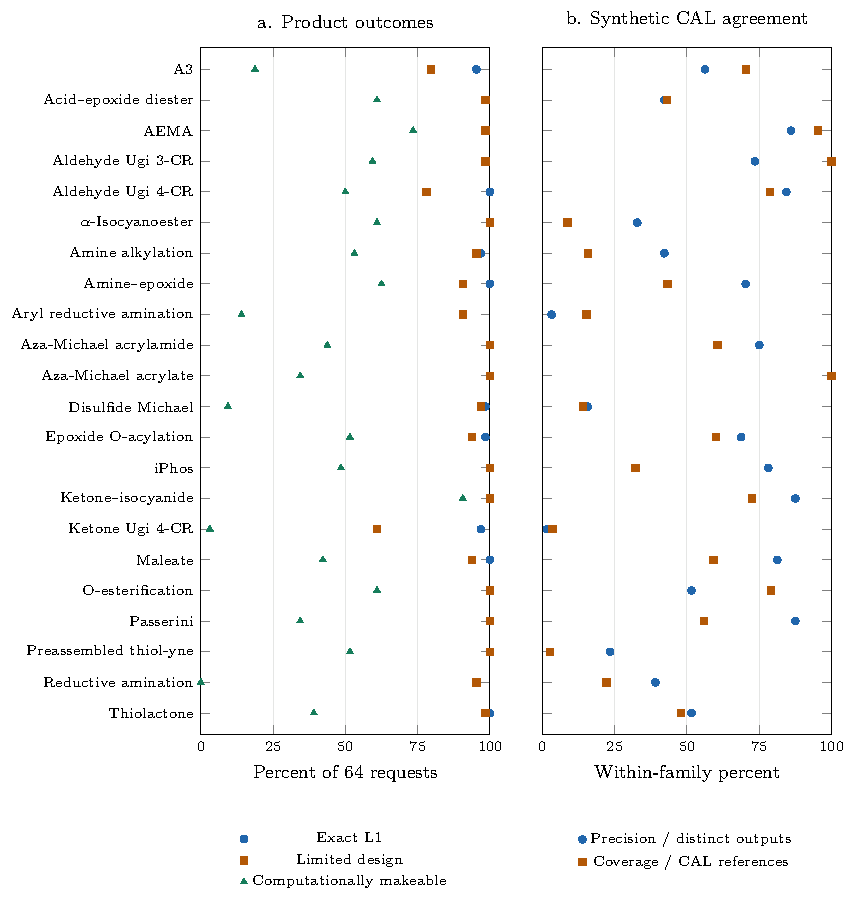
\includegraphics[width=\textwidth]{figures/current_results/family_overview.pdf}
\caption{\textbf{Current development results across 22 reaction families.}
Exact L1, limited-design and computational-makeability counts use all 64 selected requests per
family. ECFP reference precision and CAL coverage use separate generated/reference denominators.
The selected cohort is adaptively developed from one checkpoint; independent-seed and independent
held-out confirmation remain unmeasured. Assembly consistency, limited checks, reference similarity
and route evidence are separate outcomes.}
\label{fig:22-overview}\end{figure}

\subsection{Representative structures and unresolved failures}
\begin{figure}[H]\centering
\ResultPanel{a. Seeded all-family atlas}{One or more prespecified random products per family, with exact precursors and evidence depth.}\hfill
\ResultPanel{b. Paired failure analysis}{Original and repaired graphs; edits, remaining concerns and unchanged source checks.}
\caption{\textbf{Structures and failure analysis across reaction families.} A prespecified all-family atlas remains unmeasured. Existing targeted failure galleries are developmental diagnostics, not a random or method-masked quality sample. Atom origins, component novelty and L1/L2/L3 evidence require separate annotations. Molecular drawings represent exact graphs and do not establish three-dimensional stability.}
\label{fig:22-atlas}\end{figure}
The structure analysis pairs original and repaired graphs and includes oversized rings, malformed
cages, missing retained heads and joint atom/bond errors, alongside source-positive controls.
Graph and drawing hashes distinguish molecular changes from depiction corrections. Random samples
and examples selected to illustrate a specific failure are identified separately.

\subsection{Failure accounting and reproducibility}
The analysis retains failed requests and runs, unsupported chemistry, unavailable references,
source conflicts, null contrasts and search censoring. Source, configuration, checkpoint, policy and
split hashes link each result to its executable analysis and verification receipt. We distinguish
TRAIN-derived proposal and selection diagnostics from evaluation against independent references.
Passing limited structural checks does not establish complete chemical quality, stability, ionization
or delivery activity; context flags and unresolved cases remain part of the reported outcome.

